
\documentclass{article}
\usepackage[utf8]{inputenc}
\usepackage{fullpage}

%Examples
\usepackage{linguex}

%Tables
\usepackage{multirow}
\usepackage[table]{xcolor}
\definecolor{blue}{HTML}{4E60F0}
\usepackage{colortbl}

%Math
\usepackage{amssymb, stmaryrd}
\usepackage[fleqn]{amsmath}

%Graphics
\usepackage{graphicx}
\graphicspath{{./fig/}}
\usepackage{subcaption}

%Comments
%MORA
\newcommand{\changeMM}[2]{{\leavevmode\color{red}{\scriptsize\st{#1}}~\color{red}#2}}
\newcommand{\nbMM}[1]{{\leavevmode\color{red}{\scriptsize#1}}}
\newcommand{\addMM}[1]{{\leavevmode\color{red}#1}}

%EWAN
\newcommand{\changeED}[2]{{\leavevmode\color{blue}{\scriptsize\st{#1}}~\color{blue}#2}}
\newcommand{\nbED}[1]{{\leavevmode\color{blue}{\scriptsize#1}}}
\newcommand{\addED}[1]{{\leavevmode\color{blue}#1}}

%EMMANUEL
\newcommand{\changeEC}[2]{{\leavevmode\color{green}{\scriptsize\st{#1}}~\color{green}#2}}
\newcommand{\nbEC}[1]{{\leavevmode\color{green}{\scriptsize#1}}}
\newcommand{\addEC}[1]{{\leavevmode\color{green}#1}}


%References
\usepackage{hyperref}
\usepackage{cleveref}

%Line numbers
\usepackage{lineno}
\linenumbers




\title{LDA for Mouse Tracking}

\begin{document}

\maketitle
\tableofcontents

%%INTRO
\section{Introduction}
\begin{itemize}

\item In the past ten years, mouse-tracking has become a popular method to target the processes underlying decision making in different domains, ranging from phonetic competition (Spivey, Grosjean, \& Knoblich, 2005), and syntactic and pragmatic processing (Farmer, Anderson, \& Spivey, 2007; Tomlinson, Bailey, \& Bott, 2013) to social cognition (Freeman \& Ambady, 2010; Freeman, Dale, \& Farmer, 2011). 

\item In its \textbf{basic form}, the standard task used in mouse-tracking experiments is a two-alternative forced choice where participants are presented with a stimulus and then they have to make a choice using the options appearing in the top left or right corner. In each trial, participants have to press a “Start” button, located at the middle bottom of the screen, to see the stimulus. As participants move the mouse cursor to select the response, $x,y$ coordinates are recorded. 

\item Based on the assumption that motor responses are prepared in parallel to cognitive processing and performed in a cascade manner (i.e., as fast as they can be executed) (Song \& Nakayama, 2006; Freeman \& Ambady, 2010, Spivey \& Dale, 2006), mouse-tracking studies have usually assumed that mouse paths can reveal the dynamics of decision making with fine-grained temporal resolution (Freeman et al., 2011; Freeman \& Ambady, 2010; Hehman, Stolier, \& Freeman, 2014).  
As a result, certain features in mouse trajectories are thought to be indicators of specific decision patterns\footnote{In this sense, mouse trajectories are equivalent to eye movements. However, the main advantage of mouse tracking over eye tracking is the simplicity of the set up, which can be even tested online.}. 

%\item The theoretical assumption behind all these MT studies is that cognitive processes can be reflected in mouse trajectories. In other words, specific features of mouse trajectories can be associated to different cognitive patterns. 

\item For instance, whenever a decision involves two independent processes --such as a change of decision--, mouse trajectories are expected to be displayed as two movements, whereas a single smooth and graded movement would reflect a commitment with an initial choice (Wojnowicz et al., 2009).

% The general idea behind the paradigm was that the form of the trajectory to the correct response could indicate whether participants were confident with their initial decision, whether they oscillated between the two responses (i.e. they were uncertain), or whether they considered the alternative option before ultimately select the other (i.e. whether they changed their minds). 

\item An example of how a \emph{two-step} processing pattern is concluded from mouse trajectories is given in Dale and Duran (2011).  

\begin{itemize}
\item Dale and Duran (2011) compared the processing of negative and affirmative sentences to test the traditional hypothesis that negation is an operator that reverses the truth conditions of the sentence, inducing a shift in the verification strategy: truth conditions for the positive content are first derived and negated only afterwards (Wason \& Johnson-Laird, 1972, REF). 

\item The authors combined a mouse-tracking parading with a Truth Judgment Task: participants had to decide whether a general statement (e.g. \textit{Cars have (no) wings}) was true or false by clicking on two response buttons located at the top left and right corners.

\item The reasoning behind the paradigm was the following: if negation involves representing the positive argument at an early processing stage, then when participants have to verify a negative sentence such as \textit{Cars have no wings}, they should initially process the positive content and go towards the ``false'' response, flipping the direction as a second step. 

\item Dale and Duran (Experiment 1) found that negation seems to involve a ``two-step'' verification: mouse trajectories presented more shifts towards the alternative response (i.e. were less straightforward) when evaluating true negative than affirmative sentences. 

\item These results suggest that the positive argument may play an important role in negation processing (see Fischler et al. 1983; Hasson and Glucksberg 2006; Kaup et al. 2007a; Ludtke et al. 2008 for similar findings). This, however, is not necessarily the case (Nieuwland and Kuperberg, 2008). 
Whether or not the positive content of a negative sentence needs to be represented for comprehension seems to depend on the amount of contextual support given for the sentence. Specifically, the ``two-step'' processing seems to occur for sentences presented out of the blue, whereas no such effect comes about when the right contextual support is provided.  How to explain this pattern of results has been at the center of the debate in the negation processing literature (see Y. Tian and R. Breheny XX for review). 
In this paper, we will not commit to any particular explanation about why negation might or might not induce such processing switch. 

\end{itemize}

\end{itemize}

%%GOALS
\subsection{Goals} 
\begin{itemize}

\item As observed, mouse trajectories are assumed to reflect decision making (i.e. infer certain decision from paths). This association, however, has never been explicitly tested.
\textbf{In this paper, we aim to test this connection between cognition (decision making) and action (mouse trajectories)}. Are decisions reflected on trajectories? 

\item Instead of taking mouse trajectories as indicators of cognitive processes, we will \emph{manipulate} whether or not our stimuli trigger a flip in decision, and identify  the features in mouse trajectories that correlate with these flips. We reasoned that trajectories for trials that involve a change of decision should all share meaningful components. 

\item A traditional \emph{linear discriminant analysis} (henceforth, LDA) will be fed with these (already labeled) mouse trajectories. The LDA is an optimal solution to classify continuous data into two or more categories. Thus, it will allow us not only to classify mouse trajectories according to whether there was a switch of decision, but potentially also to make a second distinction between trajectories that underly a rapid commitment and trajectories that underly uncertainty.  \addMM{We won't explore this issue here}. 

\item In the last section of the paper, the LDA classifier will be further tested with new data, obtained from a replication of Dale and Duran (2011).   
\end{itemize}


%% CALIBRATION EXPERIMENT
\section{Manipulating decision making: Validation Experiment}
We developed an experiment where participants had to perform a \emph{two-alternatives forced task}: at each trial, they were presented with a coloured frame surrounding the screen and they had to determinate whether the frame was blue or red. 
Responses were made by clicking on the ``blue" or ``red" buttons, allowing the recording of mouse-movements during each trial. Importantly, responses were considered accurate if they described the color at the moment of the click. In order to mimic decision processing, we manipulated whether the color of the frame remain stable along the trial or changed at some point. An illustration of a trial is provided in \Cref{fig:trial.example}. 


\begin{figure}
\centering
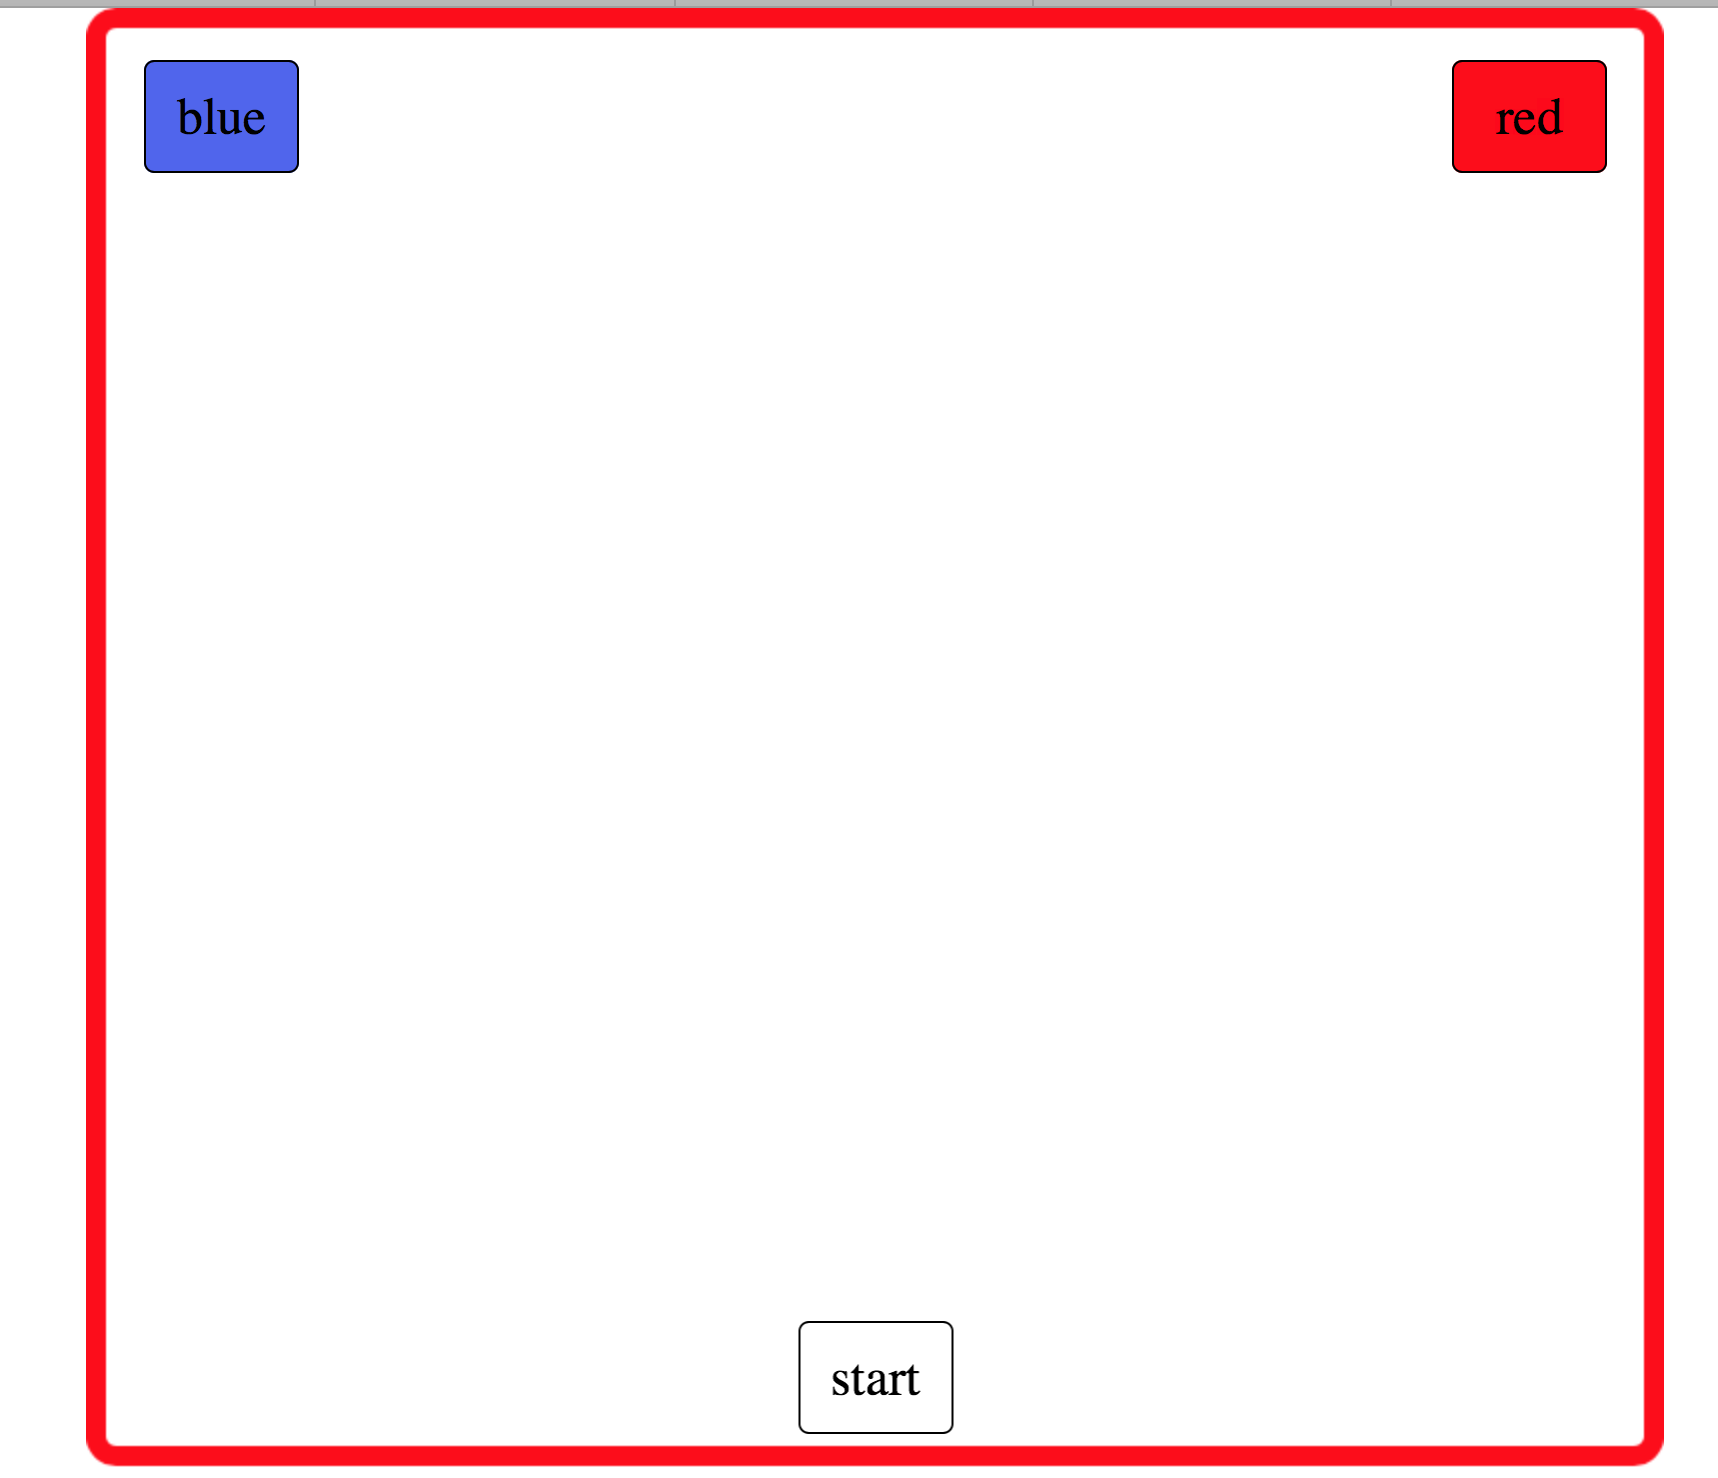
\includegraphics[scale=.2]{example_trial.png}
\caption{Example of Trial in Calibration Experiment} \label{fig:trial.example}
\end{figure}

\paragraph{Participants} 54 participants were recruited using Amazon Mechanical Turk (F=27). Two subjects were excluded from the analyses because they did not use a mouse to perform the experiment. 

\paragraph{Design}

\begin{itemize}

\item There were two \textsc{Decision Type}s: (a) \textit{Straightforward}, where the decision was made at the beginning of the trial; (b) \textit{Switched}, where the decision made at the beginning of the trial changed at some later point. 

\item The final \textsc{Frame color} (at the response moment) could be red or blue. 
\item The \textsc{Decision point} depend on the \textsc{Decision Type}. For \textit{switched} trials, there were three possible decision points: early, middle and late. These were determined by the y-position where the color changes. 
\item The proportion was adjusted so that straightforward trials were the majority  (2/3), and people could get used to make their choice right away (without staying in the middle of the screen).
\end{itemize}

\begin{table}[!h]
\centering
\begin{tabular}{cccc}
\textsc{Decision Type}&\multicolumn{2}{c}{\textsc{Frame color}}&\textsc{Decision point}\\
\hline
\multirow{2}{*}{Straightforward} & \multicolumn{2}{c}{\cellcolor{blue} Blue} & -- \\
& \multicolumn{2}{c}{\cellcolor{red} Red} & -- \\
\hline
\multirow{2}{*}{Switched} & \cellcolor{blue}Blue & \cellcolor{red} Red & early (y1=.4), middle (y2=.7), late (y3=.9) \\
 & \cellcolor{red} Red & \cellcolor{blue} Blue & early (y1=.4), middle (y2=.7), late (y3=.9) \\
\hline
\end{tabular}
\caption{Design in Calibration Experiment}
\end{table}



\paragraph{Interface}
The interface was programmed using JavaScript. Mouse movements triggered the extraction of x,y-pixel coordinates (i.e., no constant sample rate). The software was adapted proportionally to the window of the participant's browser, forming a rectangle: the height was covered at 100 percent and the width was 120 percent of the height. 
Three buttons were displayed during the experiment (\textit{start} and response buttons). Their size was also determined by the browser window (i.e., approximately 20 percent of the total width). The \textit{start} box was placed at the bottom center of the screen. The two response boxes were located at the top left (\textit{blue}) and top right (\textit{red}) corners of window. This location was constant across participants, and handedness was controlled.  
In each trial, mouse movements were recorded between start-clicks and response-clicks. The x,y-pixel trajectory was saved together with its raw time. Afterwards, the positions were normalized according to participants' window size, to allow comparisons between subjects. The normalization was done by considering the start button at the [0,0] point, the "blue" button corner at [-1,1] and the "red" button at [1,1]. 

\paragraph{Data treatment}
Mouse-tracking data are particularly variable trial to trial. On one hand, variations in response times imply different quantity of \textit{x,y} positions per trial, making difficult the comparisons between items. On the other hand, in our design, positions are extracted based on mouse movements, and devices with more or less sensibility could influence the number of samples taken during the trial. In order to compare mouse trajectories, we normalized the time course into 101 proportional times steps (percentage of trial duration). This normalization, as all the other calculations, was performed in the Spyder environment using Python 2.7. 


\subsection{Overall performance}
\begin{itemize}
\item Participants performed the task accurately, making their decision based on the colour of the frame at the time of the response. Inaccurate trials (less than 4\%) were removed from the analyses. 
\item Mean trajectories for each \textsc{decision type} and \textsc{decision point} are illustrated in \Cref{fig:mean.trajectories.calibration}. 
Temporal information about changes in the $x$ coordinate is provided in the appendix (Figure X). 
These trajectories suggest that people do react to the change of colour in the expected way; namely, they make a first decision when they see the colour frame, and revise this decision if needed. \addMM{It's unclear whether the initial decision is made as soon as they press the \textit{start} button and see the frame or if there is some initial uncertainty where participants stay in the middle of the screen.}

\end{itemize}

\section{Classifying decision processes with LDA}

\begin{figure}
\centering
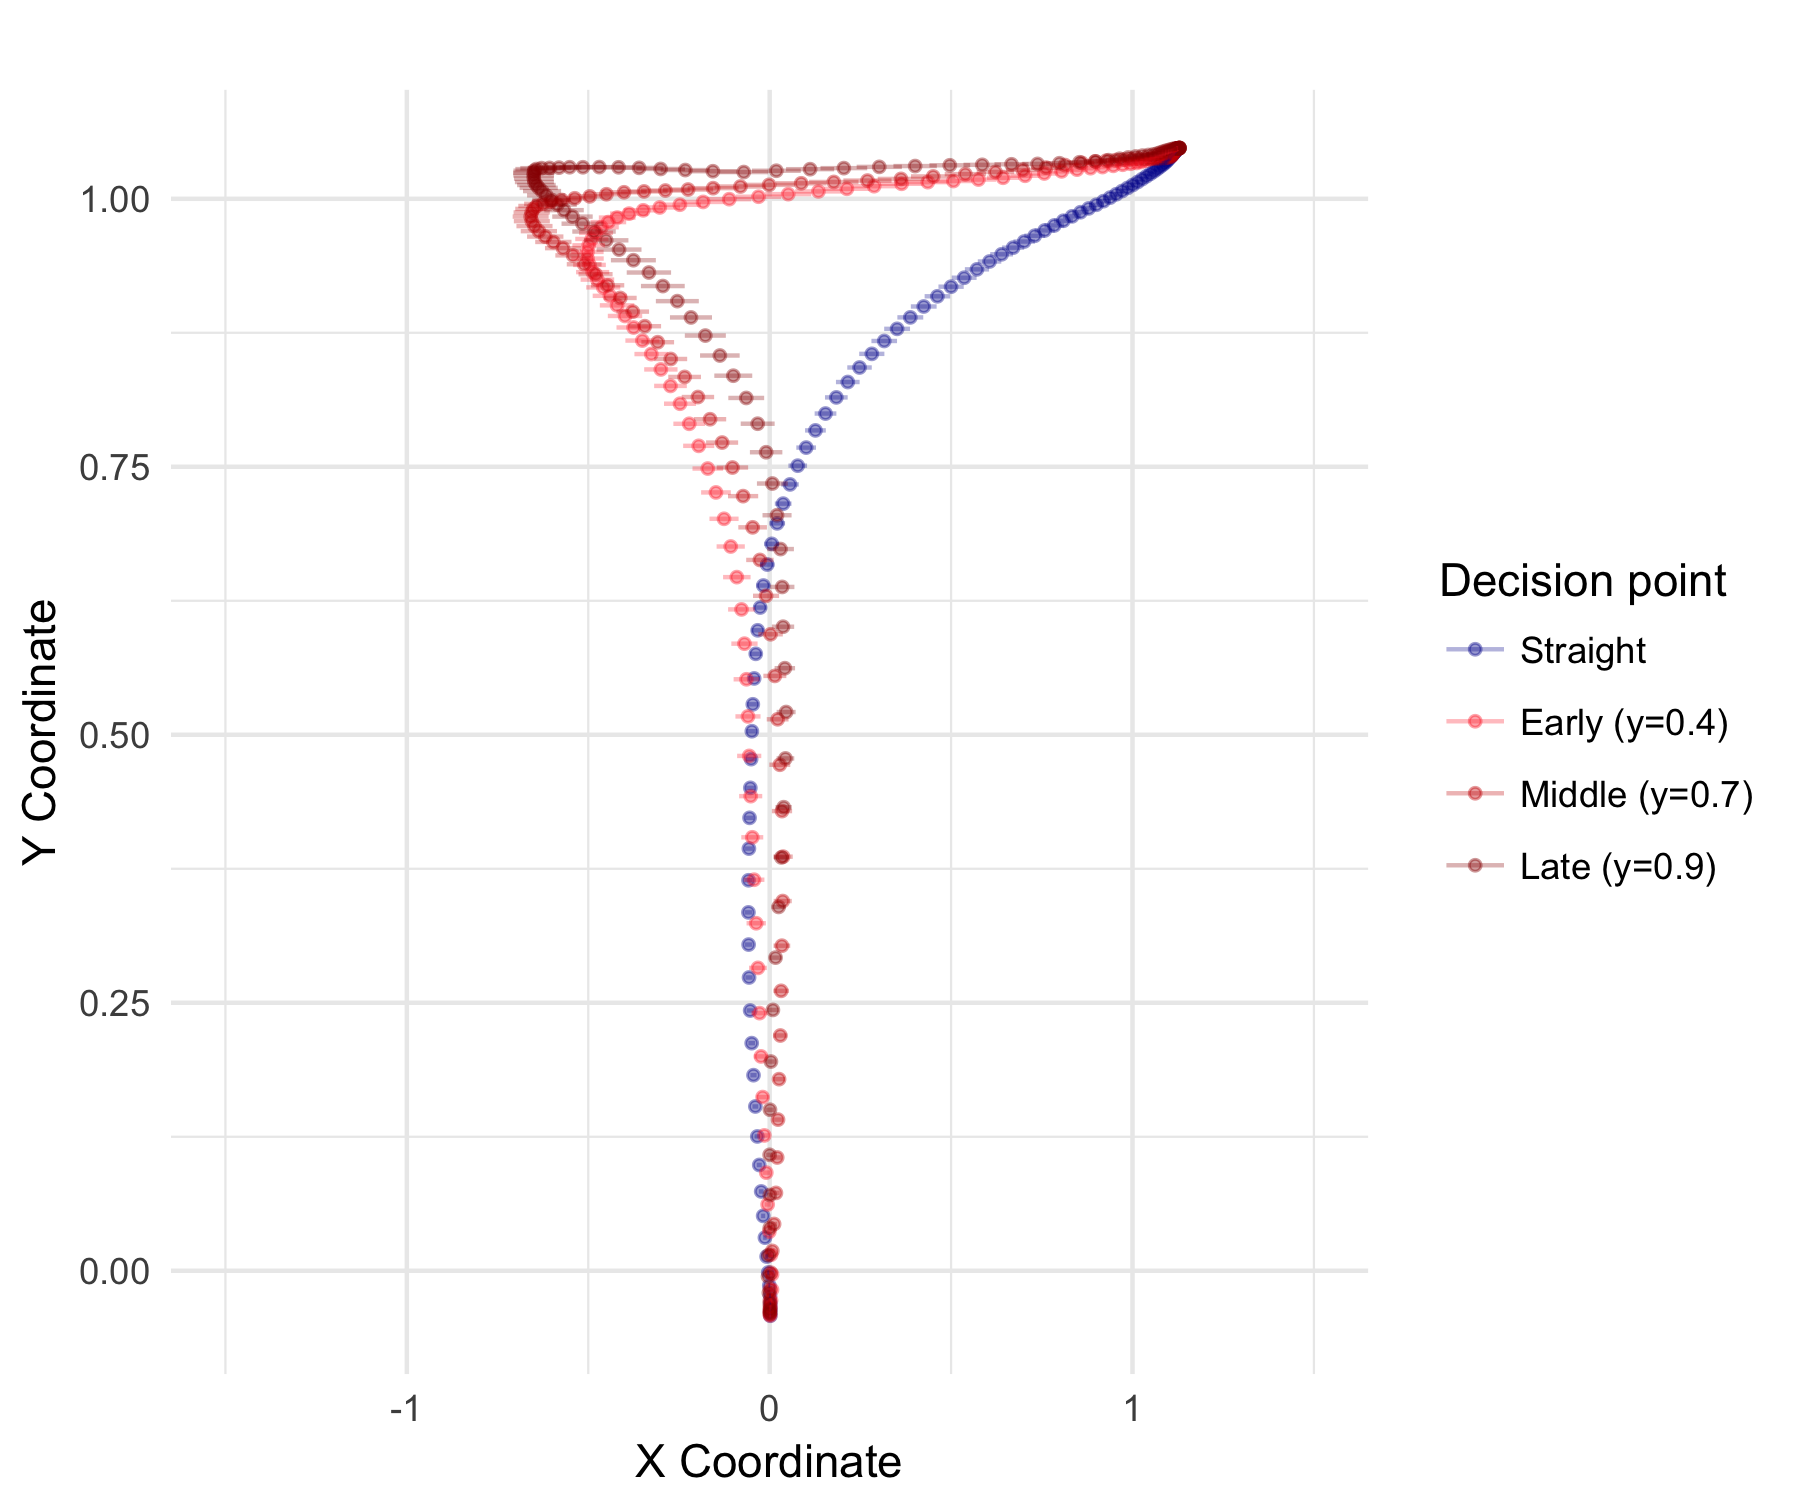
\includegraphics[width=0.7\textwidth]{calibration_mean_trajectory_pointchang.png}
\caption{Mean trajectories per class}\label{fig:mean.trajectories.calibration}
\end{figure}

%%% CLASSIFIER DESCRIPTION
\subsection{Description of LDA classifier}
\begin{itemize}
\item In order to best recognize the (mouse) patterns characteristic of each class (\textit{switched} vs. \textit{straightforward}), we use a LDA method for classification. This algorithm assumes that different classes have a common covariation matrix, and finds the linear combination of predictors that gives maximum separation between the classes.
This linear combination of predictors is obtained as a linear coefficient and it can be used to form a decision rule. 

\item The predictors used by the classification algorithm were (a) the \textit{x,y} coordinates, (b) Euclidean-based velocity, and (c) Euclidean-based acceleration. Trajectories were labeled in two classes: \emph{straightforward} and \emph{switched}. \addMM{The idea being that coordinates give us information about where the mouse is when, while acceleration and speed give us information about how did we arrive there.}

\item To avoid collinearity issues, we used a PCA to identified 13 principal components on the features describe above. We perform the LDA on these 13 components. 
We obtained a \emph{LDA measure} for each trial by calculating the dot product of the linear coefficient of the PCs and the PCs themselves. 

%\addMM{
%The procedure used to obtain a LDA measure was done as follows:
%\begin{enumerate}
%\item Remove dimensions that are constant between groups (coordinates that don’t change) and correlated dimensions between groups. 
%\item Identify the 13 principal components on the data (PCA). 
%\item Perform a LDA (linear discriminant analysis): Linear combination of the 13 PCA (predictors) that gives maximal separation between \emph{Decision change} and \emph{No decision change} classes.
%\item Extract the bias: bias = $mean \ (\text{LDA/PC}_{1\times 13} \ast \text{PC/trial}_{13\times n})$
%\item Obtain the \emph{LDA measure} per trial by calculating the dot product of the linear coefficients for each PC ($1\times13$ matrix) and the each PC for trial ($13 \times n$ matrix) minus the bias. \\
%LDA measure = \( \text{LDA/PC}_{1\times 13} \ast \text{PC/trial}_{13\times n} -  mean \ (\text{LDA/PC}_{1\times 13} \ast \text{PC/trial}_{13\times n}) \)
%\end{enumerate}}

\end{itemize}

%%%% CLASSIFIER PERFOMANCE

\subsection{Classifier performance} 

\begin{itemize}
\item The distribution and mean \textit{LDA measures} for the trajectories of each condition are illustrated in \Cref{DIST:LDA}. 

\item The overall performance of the classifier was evaluated by calculating the area under the ROC curve. The ROC curve diagnose the classification ability as a function of the degree of sensitivity (percentage of change-of-mind trajectories correctly identified) and specificity (percentage of rapid-decision trajectories correctly identified) of the classifier. Given that an ideal ROC curve will hug the top left corner, the larger the AUC the better the classifier performance. 

\item The calibration data was partitionated into 10 bins that kept the proportion of \textit{straightforward} and \textit{switched} trajectories constant (75/25 proportion). For each bin, we took the complementary set of data (the rest 90\%) to train the classifier. The data contained in the bin was used as test set to diagnose the classifier performance. In other words, we obtained a ROC curve and its AUC for each test bin (n=10). \Cref{ROC:LDA} shows the resulting ROC curves for each of the 10 bins.  

\item The performance of the LDA classifier was compared to \emph{baseline}, equivalent the worst possible outcome, and a \emph{topline}, which was what we would expect from the classifier under the best possible conditions. 
For the baseline, we used a random classifier that assigned labels by sampling from a beta distribution centred at the `straightforward' probability; the topline was computed by testing and training the original LDA classifier with the same set of data. 

\item To assess whether the performance of the LDA classifier was different from the baseline and from the topline, we calculated the difference in AUC means between each pair of classifiers and tested it against the distribution of the possible mean-differences observable when the outcome is independent from the classifier (null hypothesis). 
The sampling distribution under the null hypothesis was computed by a resampling the observed data (`permutation distribution'). 

\item \Cref{table:comparisons.permutation.1}a shows the mean AUCs, the mean differences between the original LDA and each alternative classifier, and the p-value obtained by performing a one-tail test on the data. As expected, our original LDA is significantly better than the random classifier at categorizing trajectories. Conversely, there is no significant difference between the performance of our LDA and the topline, suggesting that our LDA is not different from the best possible classification. 

\end{itemize}

\begin{figure}
\begin{subfigure}[b]{0.55\textwidth}
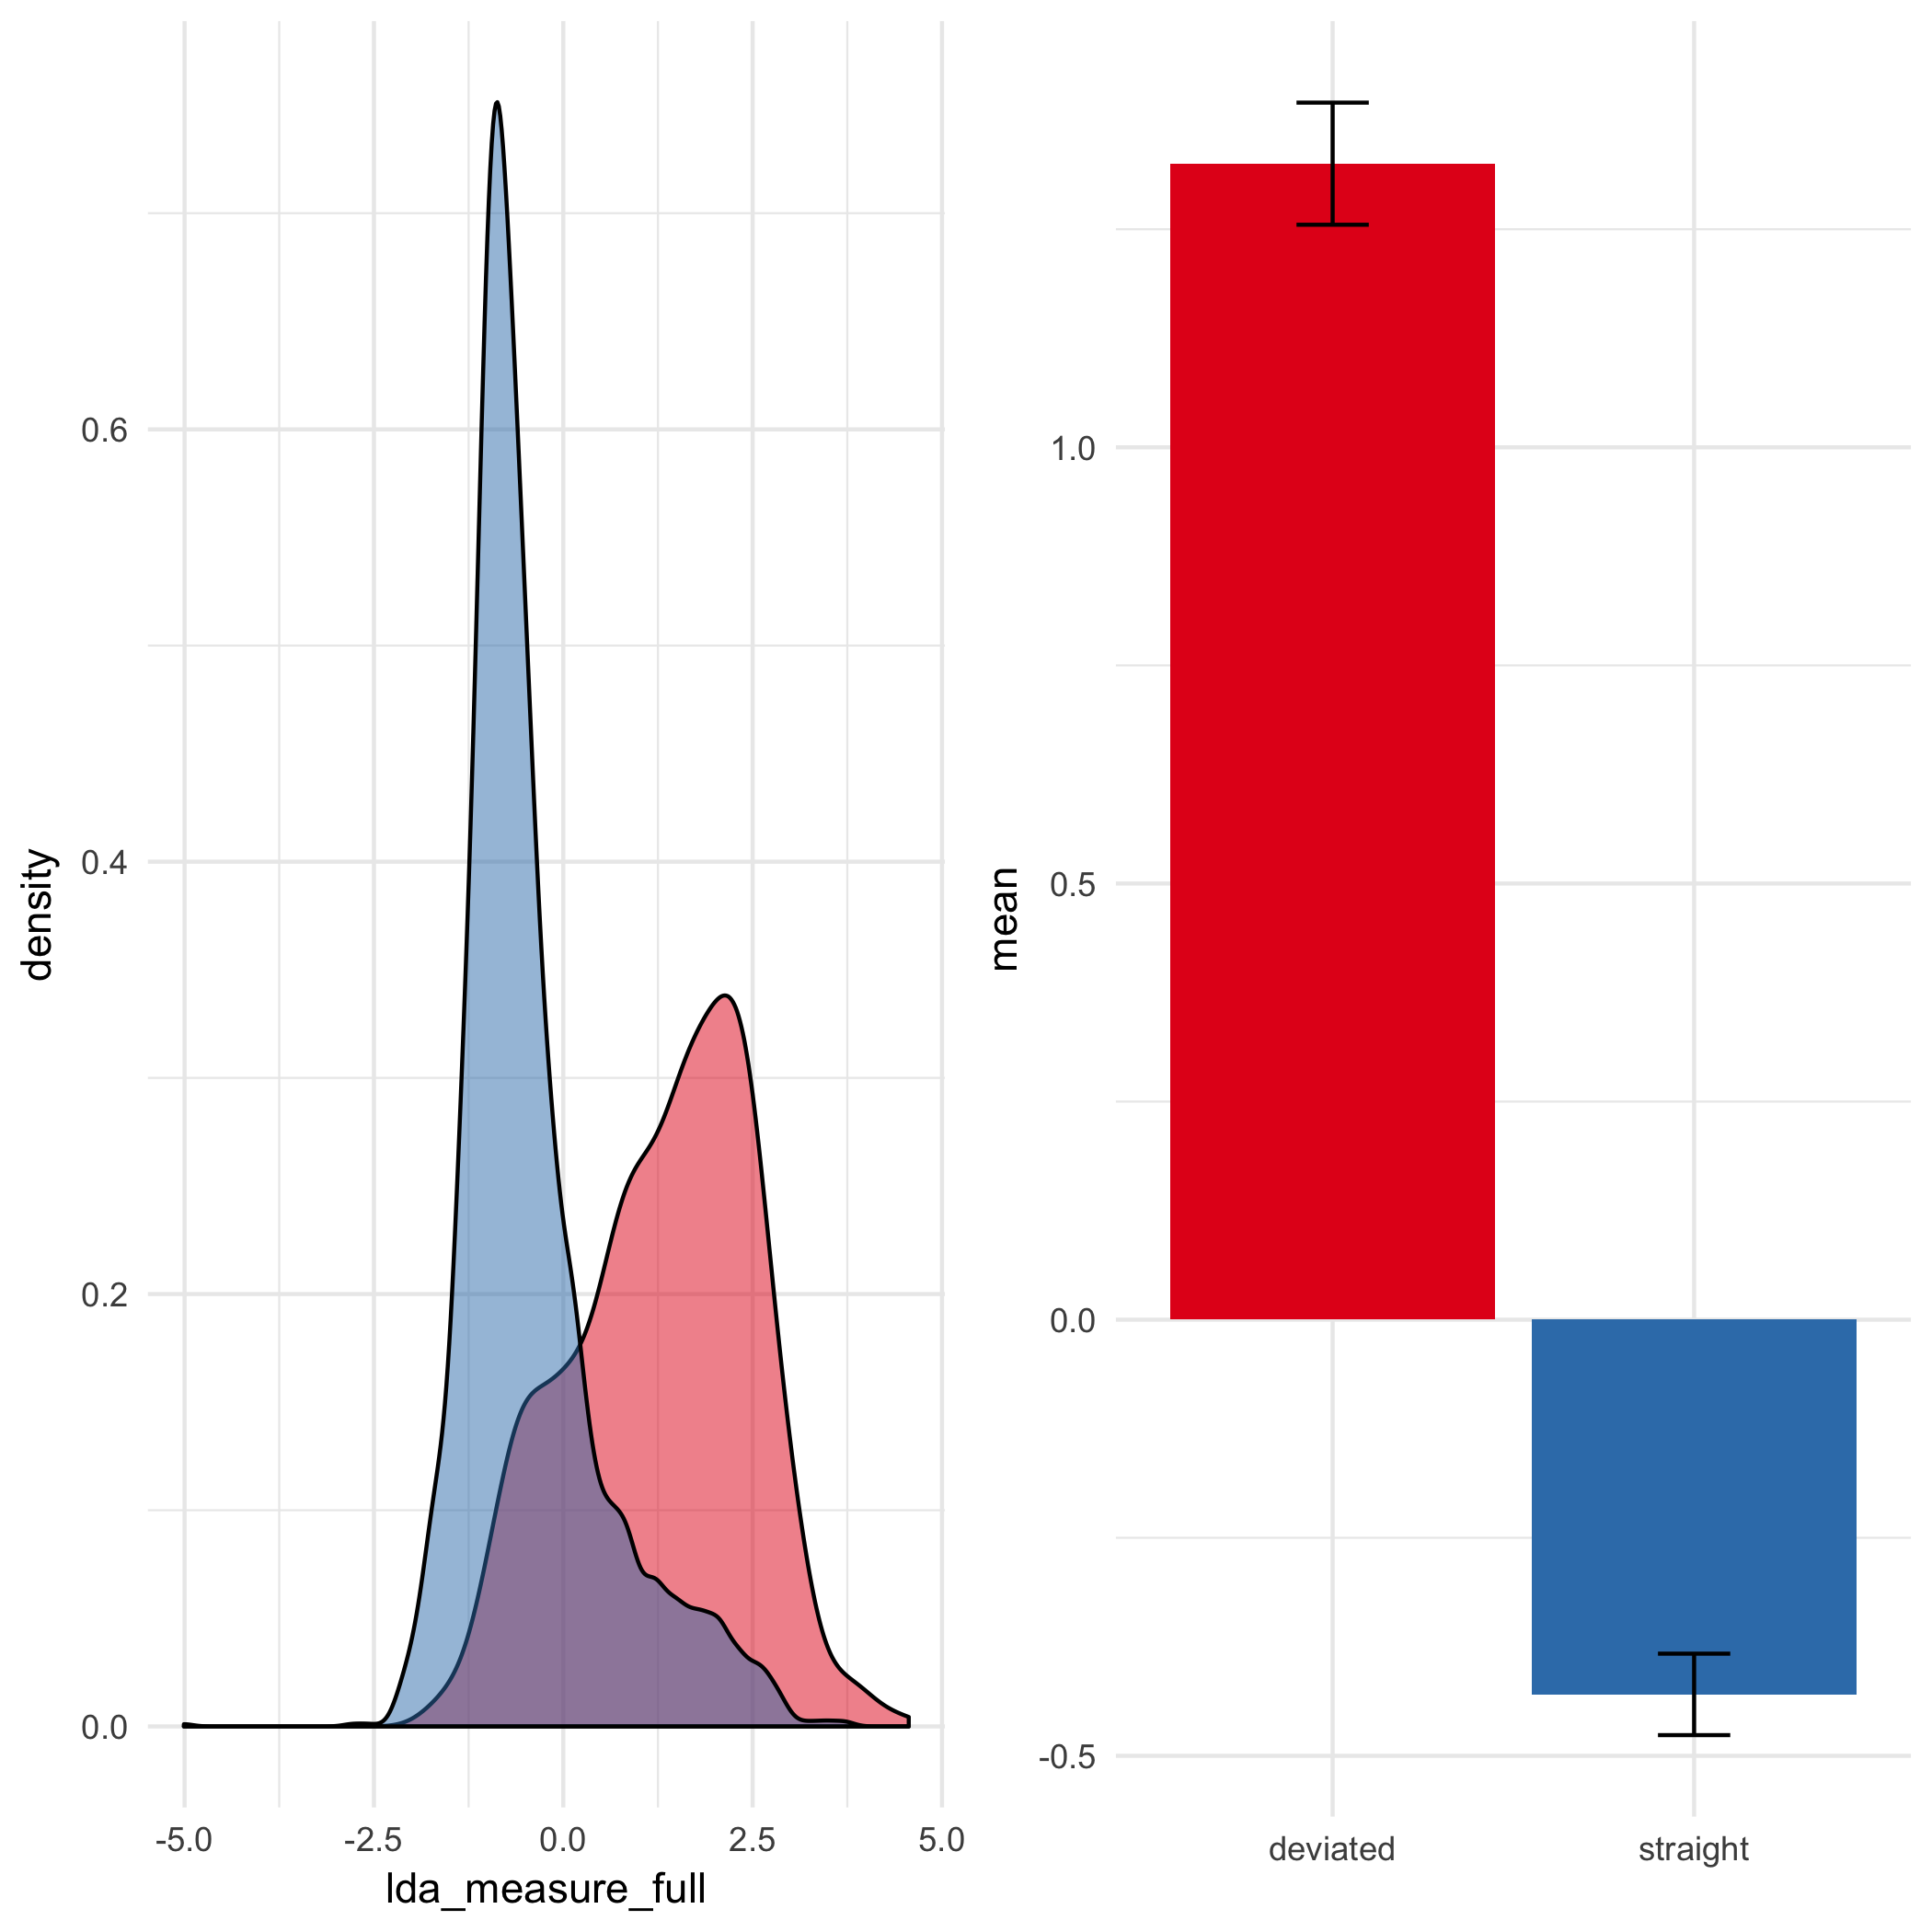
\includegraphics[width=\textwidth]{LDA-Distribution.png}
\caption{Distribution and mean for LDA measure}\label{DIST:LDA}
\end{subfigure}
%
\begin{subfigure}[b]{0.35\textwidth}
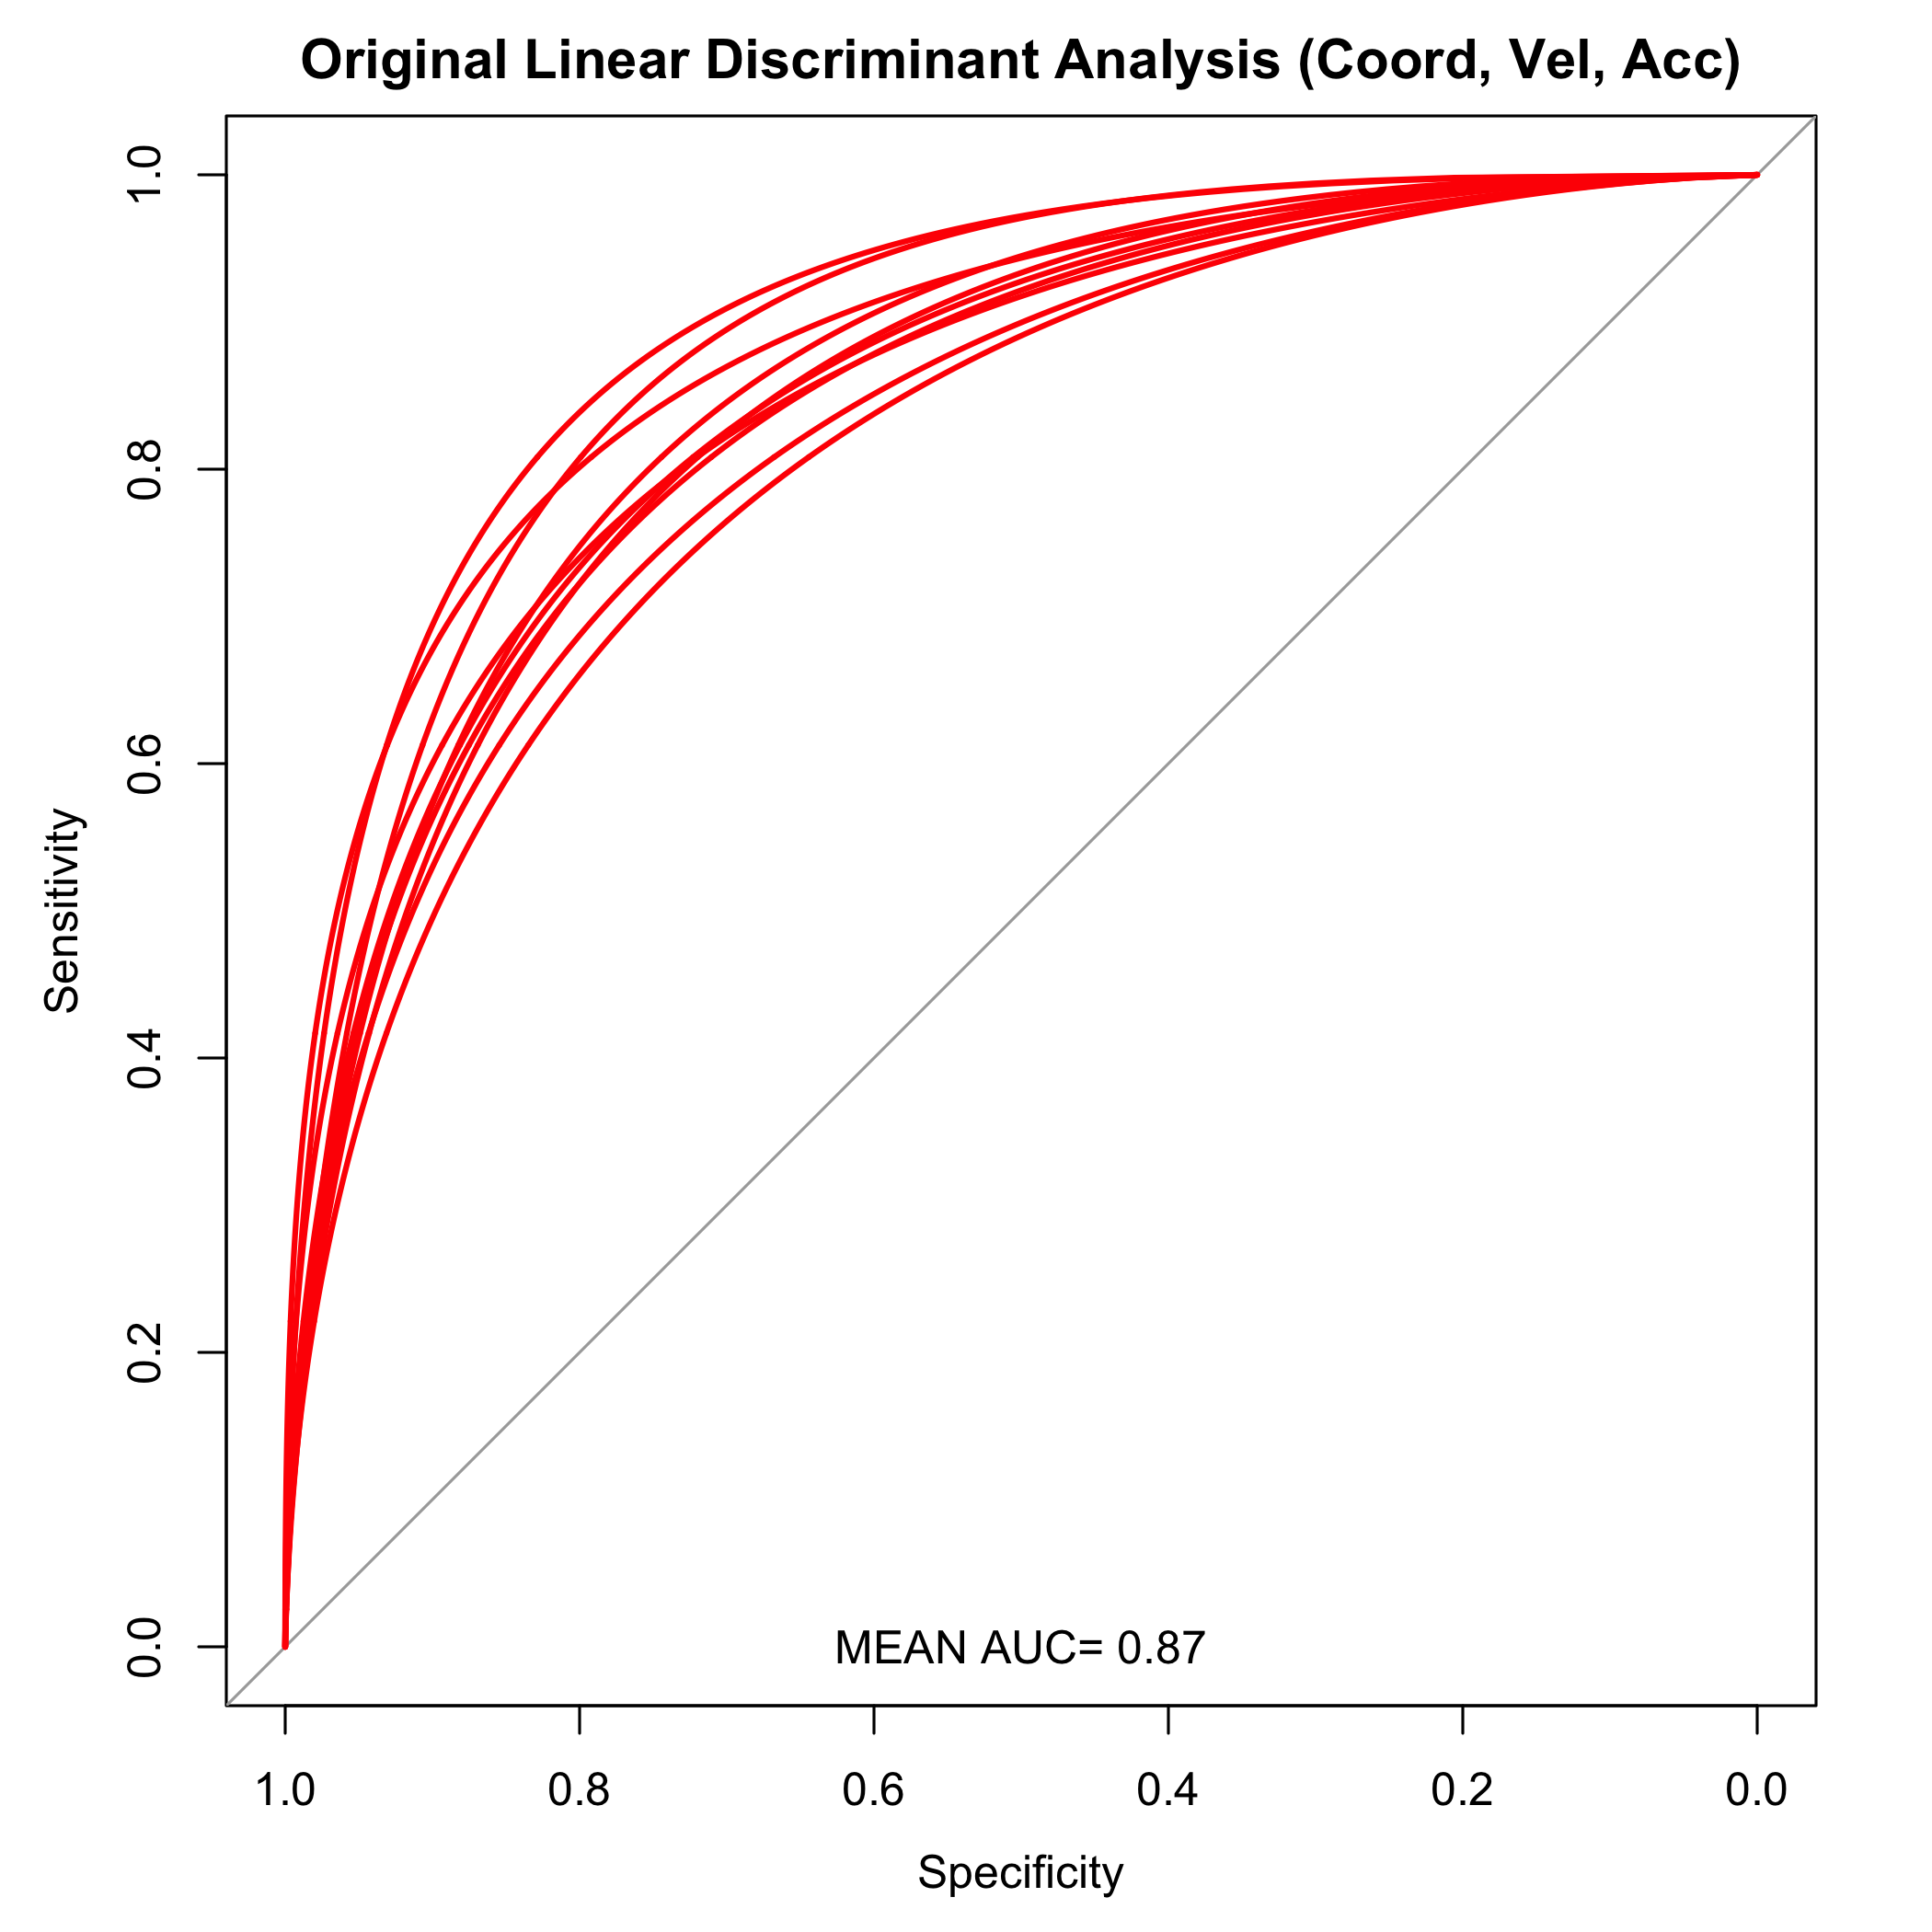
\includegraphics[width=\textwidth]{ROC_LDA-FULL.png}
\caption{ROC and AUC for the LDA measure}\label{ROC:LDA}
\end{subfigure}
\caption{Performance of the LDA classifier.}
\end{figure}


\begin{table}[h]
\centering
\begin{tabular}{p{2cm}>{\columncolor[gray]{0.8}}p{1.5cm}cc|p{1.2cm}cccc|}

 \multicolumn{2}{c}{ } &  \multicolumn{2}{c}{(a)} & \multicolumn{4}{c}{(b)}\\
\hline
& \centering \textsc{Original LDA}& \multirow{2}{1.5cm}{\centering \textsc{Baseline}} & \multirow{2}{1.5cm}{\textsc{Topline}} &\multicolumn{5}{c|}{\textsc{LDA with different predictors}}\\
\cline{5-9}
& \centering (coords, speed, acc) &  & & \centering coords, vel & vel, acc & coords & vel & acc \\[0.5cm]
%& \centering coords, delta, deltadelta & logratio  
\hline
\centering \textbf{AUC (mean)} & \centering .87& .52 & .87 &\centering .87 & .83 & .87 & .82 & .67 \\[0.5cm]
%& .88 & .84  \\[0.5cm]
\hline
\centering \textbf{Mean \\ Difference} & - & .35 & -.002 & -.0004 &  .04 & -.006 & .04 & .2 \\[0.5cm]

%& -.006 & .05   \\[0.5cm]

\hline
\centering \textbf{$p$ value} & -  &  $<$.001 & 0.58 & \centering .5 & $<$.001 & .68 & $<$.001 & $<$.001 \\
%& .72 & $<$.001 \\
\hline
\end{tabular}
\caption{Cross-validation results for the LDA classifier. The performance of the LDA was compared to the one of (a) Random and Topline classifiers and (b) LDA classifiers with different predictors.}
\label{table:comparisons.permutation.1}
\end{table}

\subsection{Meaningful features and optimal predictors}

\begin{itemize}
%position - spatial features
%timing - absolute timing
%relative temporal features - rate
\item Our original LDA classifier takes as predictors both absolute and relative spatio-temporal features (coordinates, speed and acceleration). 
While $x,y$ coordinates provide information about the absolute mouse position at each specific time step (\emph{where} and \emph{when} questions), speed and acceleration contribute to knowing how one has arrived to a given position (\emph{how} question). 
Some of these features, however, might not be relevant for the classification. 
By comparing classifiers trained with different predictors, we can gather information about which features of mouse trajectories are more relevant for distinguishing between decision processes. 

\item The performance of these additional classifiers was diagnosed in the same way as before, by computing the AUC for each of the 10 test bins. Pair-wise comparisons with the original LDA were done by testing whether the observed mean differences could have been drawn from the distribution under the null hypothesis. (by permutation test).

\item We trained five additional classifiers obtained by subsetting the three original LDA predictors. If both absolute and relative features are required to predict the decision type, we would expect our original LDA classifier to be better than any other classifier that takes only a subset of these original predictors. 

\item  \Cref{table:comparisons.permutation.1}(b) summarises the comparisons between each of these classifiers and our original LDA. 	
The original LDA does not significantly differ from classifiers that contain the coordinates among their predictors, suggesting that the distinction between \emph{straightforward} and \emph{switched} trajectories can be solely explained by the information contained in the $x,y$ coordinates. 
In contrast, the original LDA is significantly better than classifiers which use only speed and acceleration as predictors.\nbMM{Should we say something about the fact that the difference with the vel,acc and vel classifiers is significant but not particularly big?}. These comparisons therefore reveal that, for classifying our data, absolute spatio-temporal features ($x,y$ coordinates) are generally better predictors than relative features (speed and acceleration). \addMM{That is to say, it seems to be more relevant to know where are you when than how did you get there}.  

\item Note that this does not mean that changes in decision across the board do not have an impact on speed and acceleration. Indeed, it has been suggested that the speed and acceleration components can capture the level of commitment towards specific responses, such that a change of decision (\textit{swiched} trajectories) might have associated certain speed/acceleration dynamics (Hehman et al 2014). 
\addMM{However, our data are not well classified by the these components. This could be due either to the specific type of decision processes we are capturing or by the fact that our data are too noisy to be able to see differences in speed and acceleration (relation with the fact that we have online data).}

%\item There was no significant difference between our classifier and the one with partial derivatives as predictors. This indicates that speed and acceleration based on distance are not different from speed and acceleration for each specific axis. This makes sense given the observation above. 

%\item \addMM{LDA with logratio?}


\end{itemize}

\section{LDA \emph{versus} traditional mouse-tracking analyses}

\begin{itemize}

\item The LDA classifier is \emph{a priori} the optimal solution to the type of discrimination problem examined here. However, when addressing the question of whether a change of decision has occurred, previous studies have used alternative techniques to analyse mouse trajectories. In what follows, we will compare the performance of our LDA-classifier to the one of other five measures commonly used in mouse tracking studies. 

\item Following the review in Hehlman et al. (2014), we can distinguish two main types of measures, those based on spatial analyses and those based on temporal analyses. 

\begin{itemize}
\item \textbf{Spatial analyses} rely on the $x,y$ coordinates themselves and their distance to each of the possible responses (target response and alternative response). They evaluate the degree of unpredictability and complexity of the path. 

The two most popular spatial measures are the \textit{Area Under the Curve} and the \textit{Maximal deviation point}. The AUC is the geometric area between the observed mouse-trajectory and an idealised straight-line trajectory drawn from the start to the end point. Higher values are associated with higher deviation peaks towards the alternative; values closer to zero (or below) suggest trajectory close to ideal. 
The Maximal Deviation (MD) is the point that maximizes the distance between the path and the ideal trajectory.  
The number of times the trajectories goes back and forth along the x-axis has been also been used as an indicator of the complexity of the trajectory (\emph{number of x-flips}, Dale and Duran 2011).

\ex. 
\a. AUC \(= \sum (x_{t} -  x_{t-1})( y_{t} + y_{t-1})/2  - \text{AUC}_{\text{ideal trajectory}} \)
\b.  x-flips  \(= \sum H[(x_{t} - x_{t-1})(x_{t-1} - x_{t-2})] \)
\c. Acceleration flips \(= (\sum H[( a_{t} - a_{t-1})( a_{t-1} - a_{t-2})])-1 \)

\item While these measures can asses the degree of complexity of the path, they might not be able to distinguish between `two-step' and `uncertain' decision processes --i.e., trajectories with a true deviation to the alternative or centred on the middle of the screen. \\
Moreover, these measures do not have very good temporal resolution.  
For instance, a late medium-size deviation towards the alternative could underly a two-step decision whereas an early but big-size deviation towards the alternative might very well be considered just noise. However, measures such as the maximal deviation point might not be able to make a significant distinction between them. 

\item A slightly better way of assessing whether trajectories have a meaningful deviation towards the alternative response is to measure the \textit{ratio of the target distance to the alternative distance} for each $x,y$ position.  While ratio values closer to 1 suggest a position near the middle, higher values indicate a deviation towards the alternative response. Here, we extract the maximal log-ratio value per trial.  

\item \textbf{Temporal measurements} such as speed and acceleration have served to address the degree of competition at different time steps. 
Stronger competition between alternative responses is typically translated into steeper  acceleration peaks (Hehman et al., 2014). In addition, the decision point has also been associated with temporal measures such as acceleration peak and time of highest spatial deviation, either maximum ratio or maximum deviation. Importantly, in the former case, the decision is considered to appear just after the maximal deviation/maximal ratio point, whereas last acceleration peaks are typically after.
The \emph{acceleration component} is generally analized (Dale and Duran 2011, and other studies on error correction) as a function of the number of changes in acceleration (NB: This is not the same as computing the number of times the acceleration changes direction, going from positive to negative acceleration, as D\&D claim).%greater acceleration
\\
Following the procedure in Dale and Duran (2011), trajectory velocity and acceleration were computed using the distance (in pixels) covered per second over a moving window of six $x,y$ pixel coordinates. The number of acceleration flips were calculated on this smoothed acceleration. 

\end{itemize}

\item Validation data was analysed for each of these measures. \Cref{fig:different.measures} illustrates the distribution and mean values for each of our classes.


\begin{figure}
\centering

\begin{subfigure}[b]{0.45\textwidth}
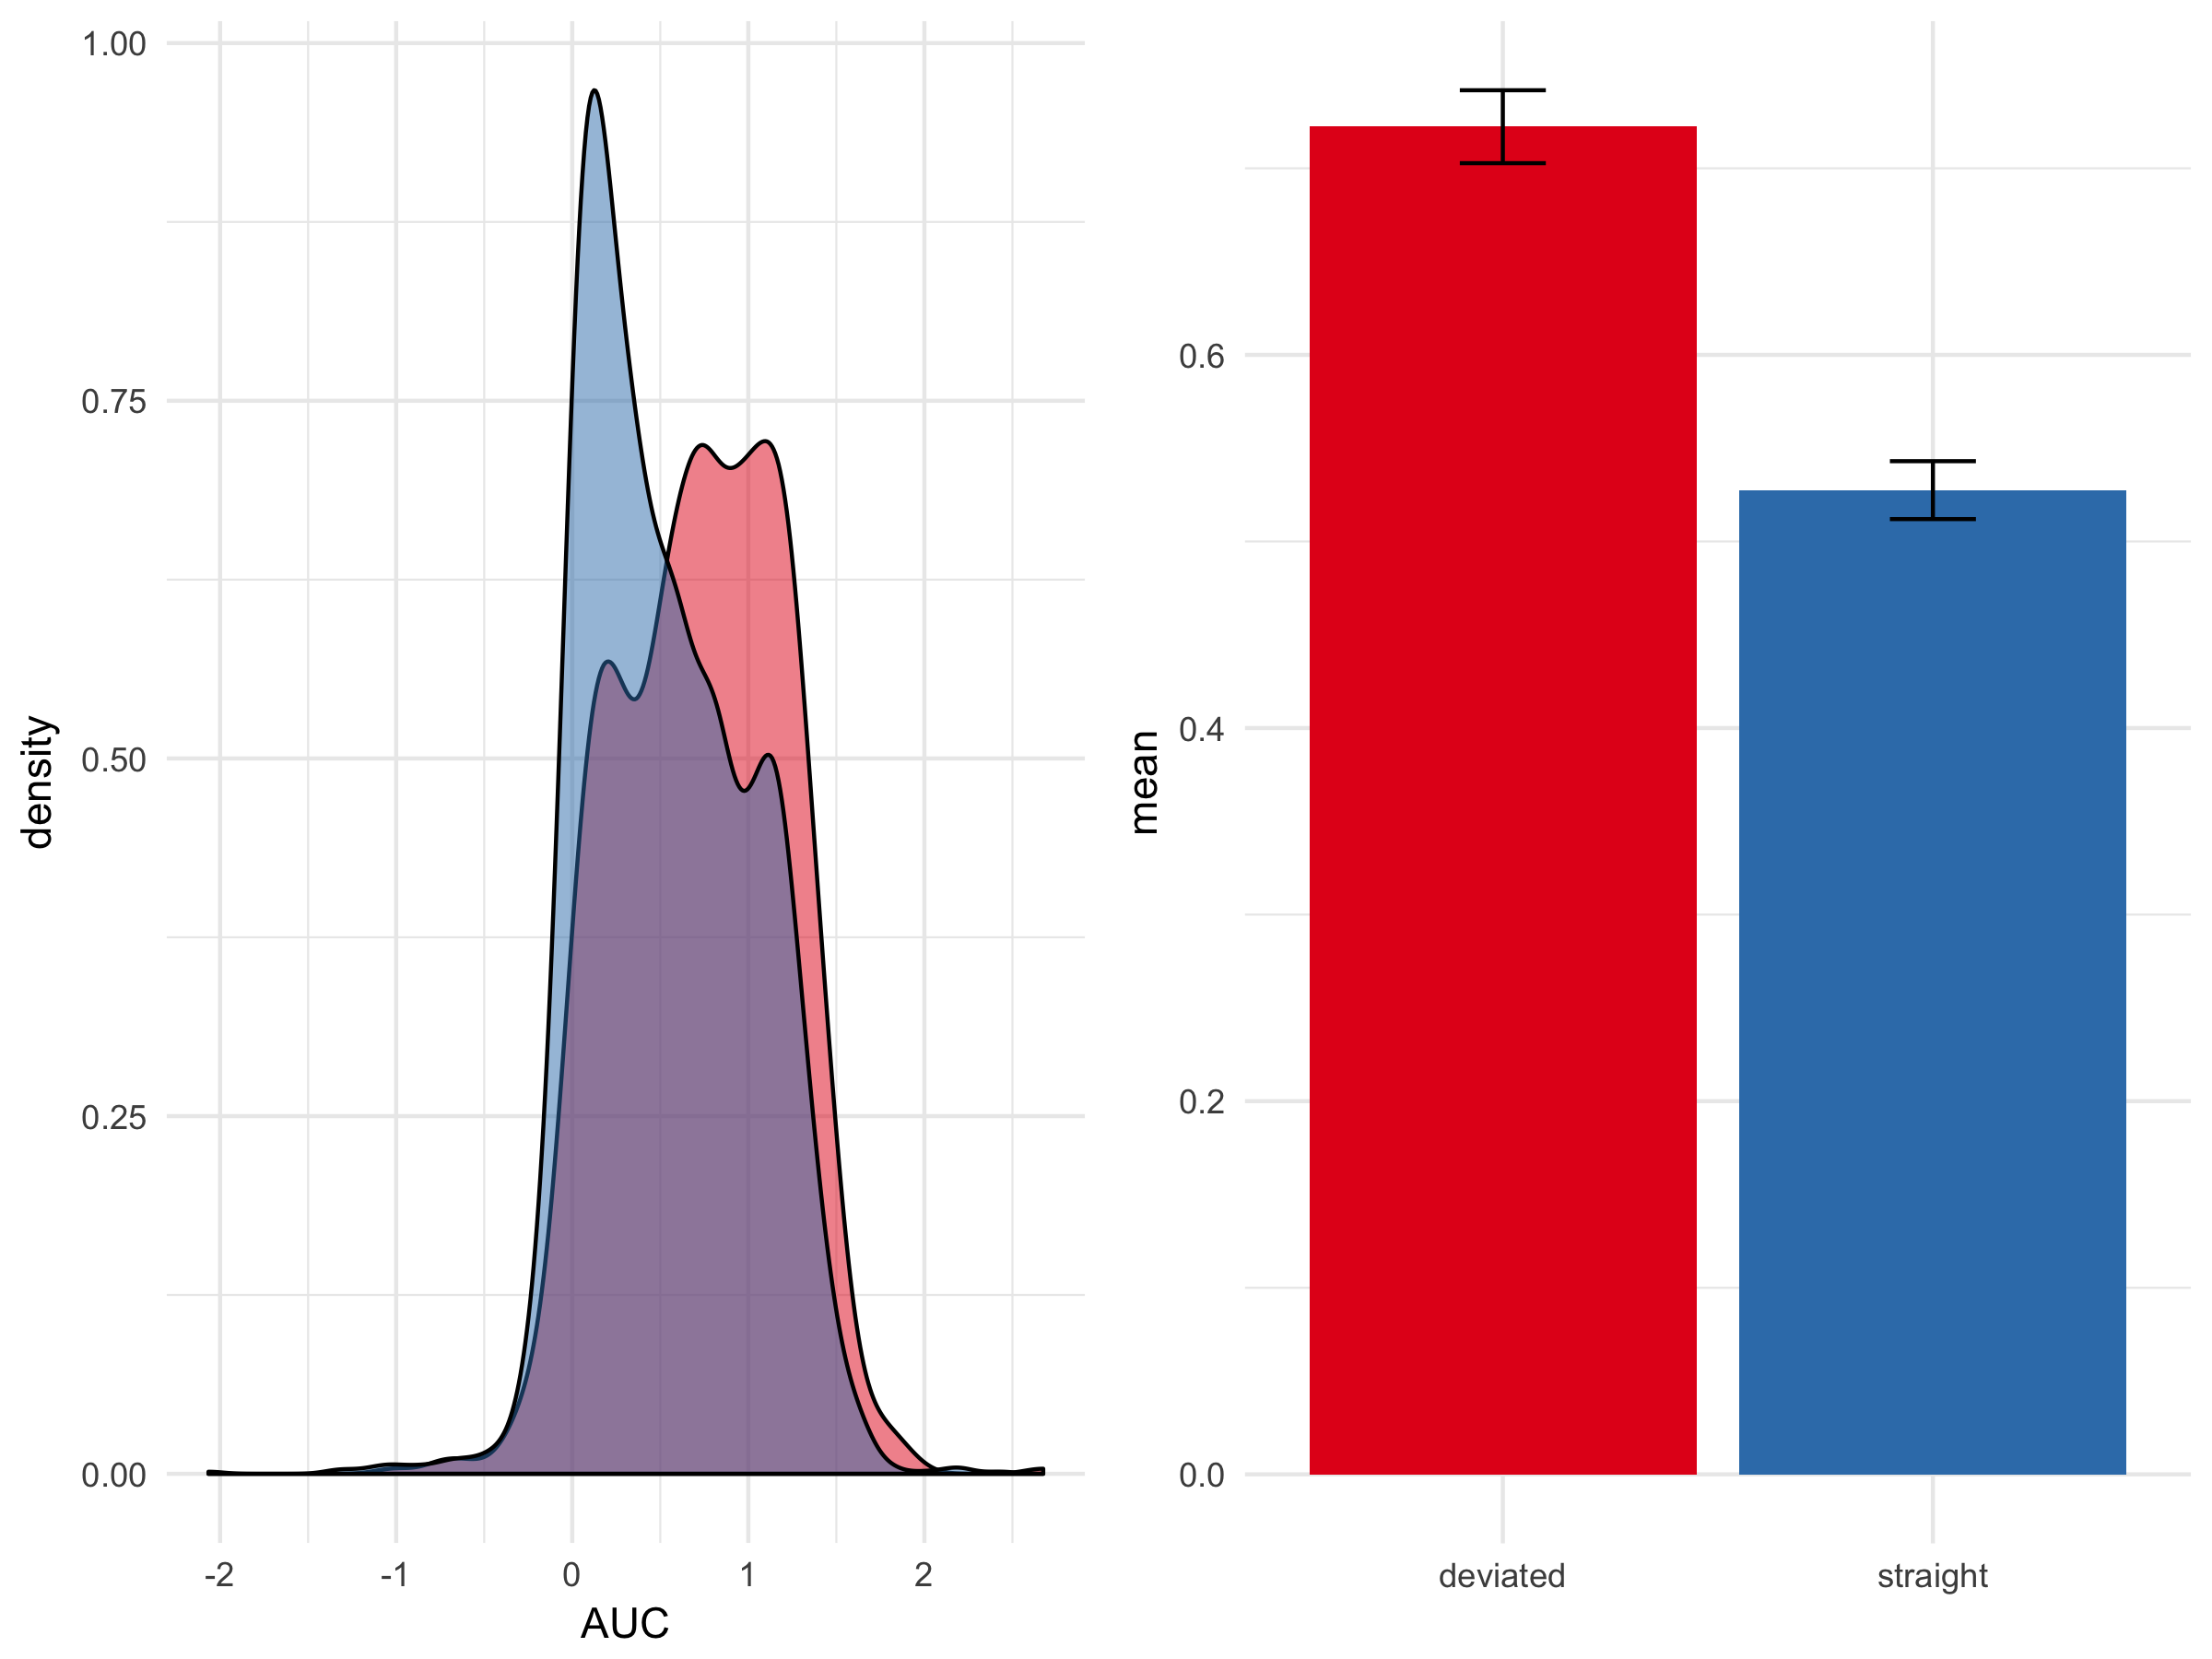
\includegraphics[width=\textwidth]{AUC-calibration.png}
\caption{Area Under the Curve}
\end{subfigure}
%
\begin{subfigure}[b]{0.45\textwidth}
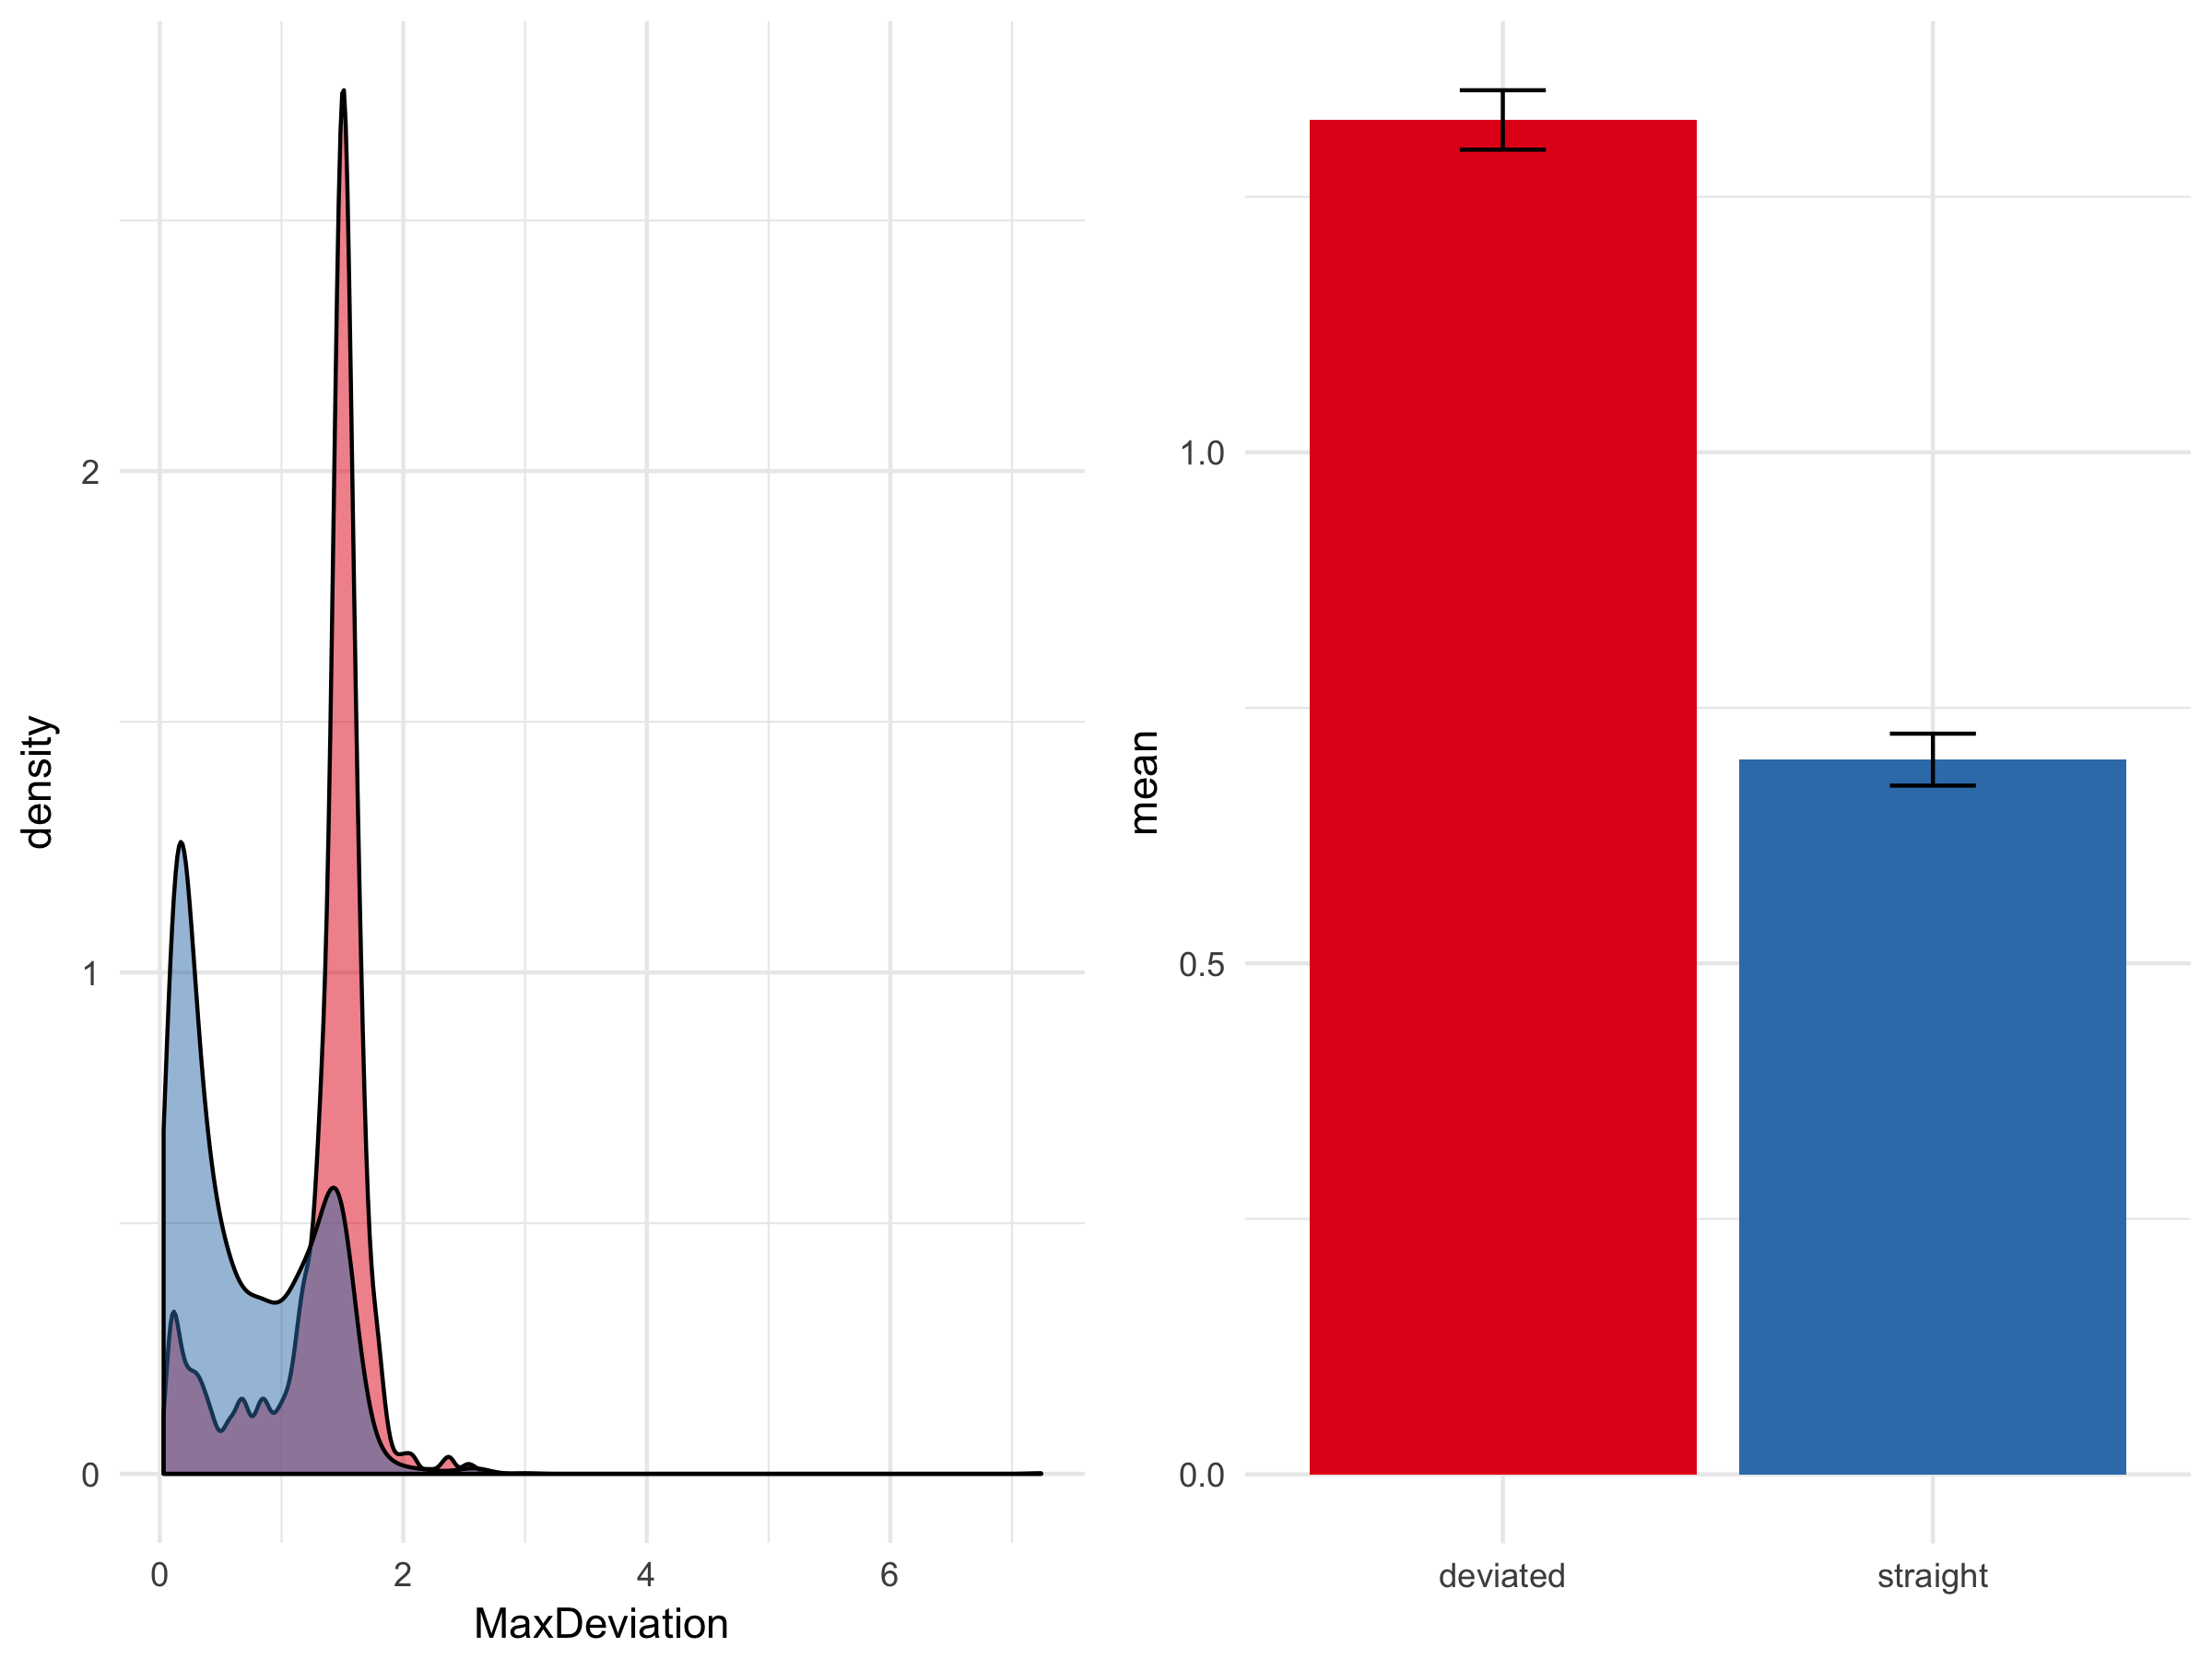
\includegraphics[width=\textwidth]{MaxDeviation-calibration.png}
\caption{Maximal Deviation}
\end{subfigure}
%
\begin{subfigure}[b]{0.45\textwidth}
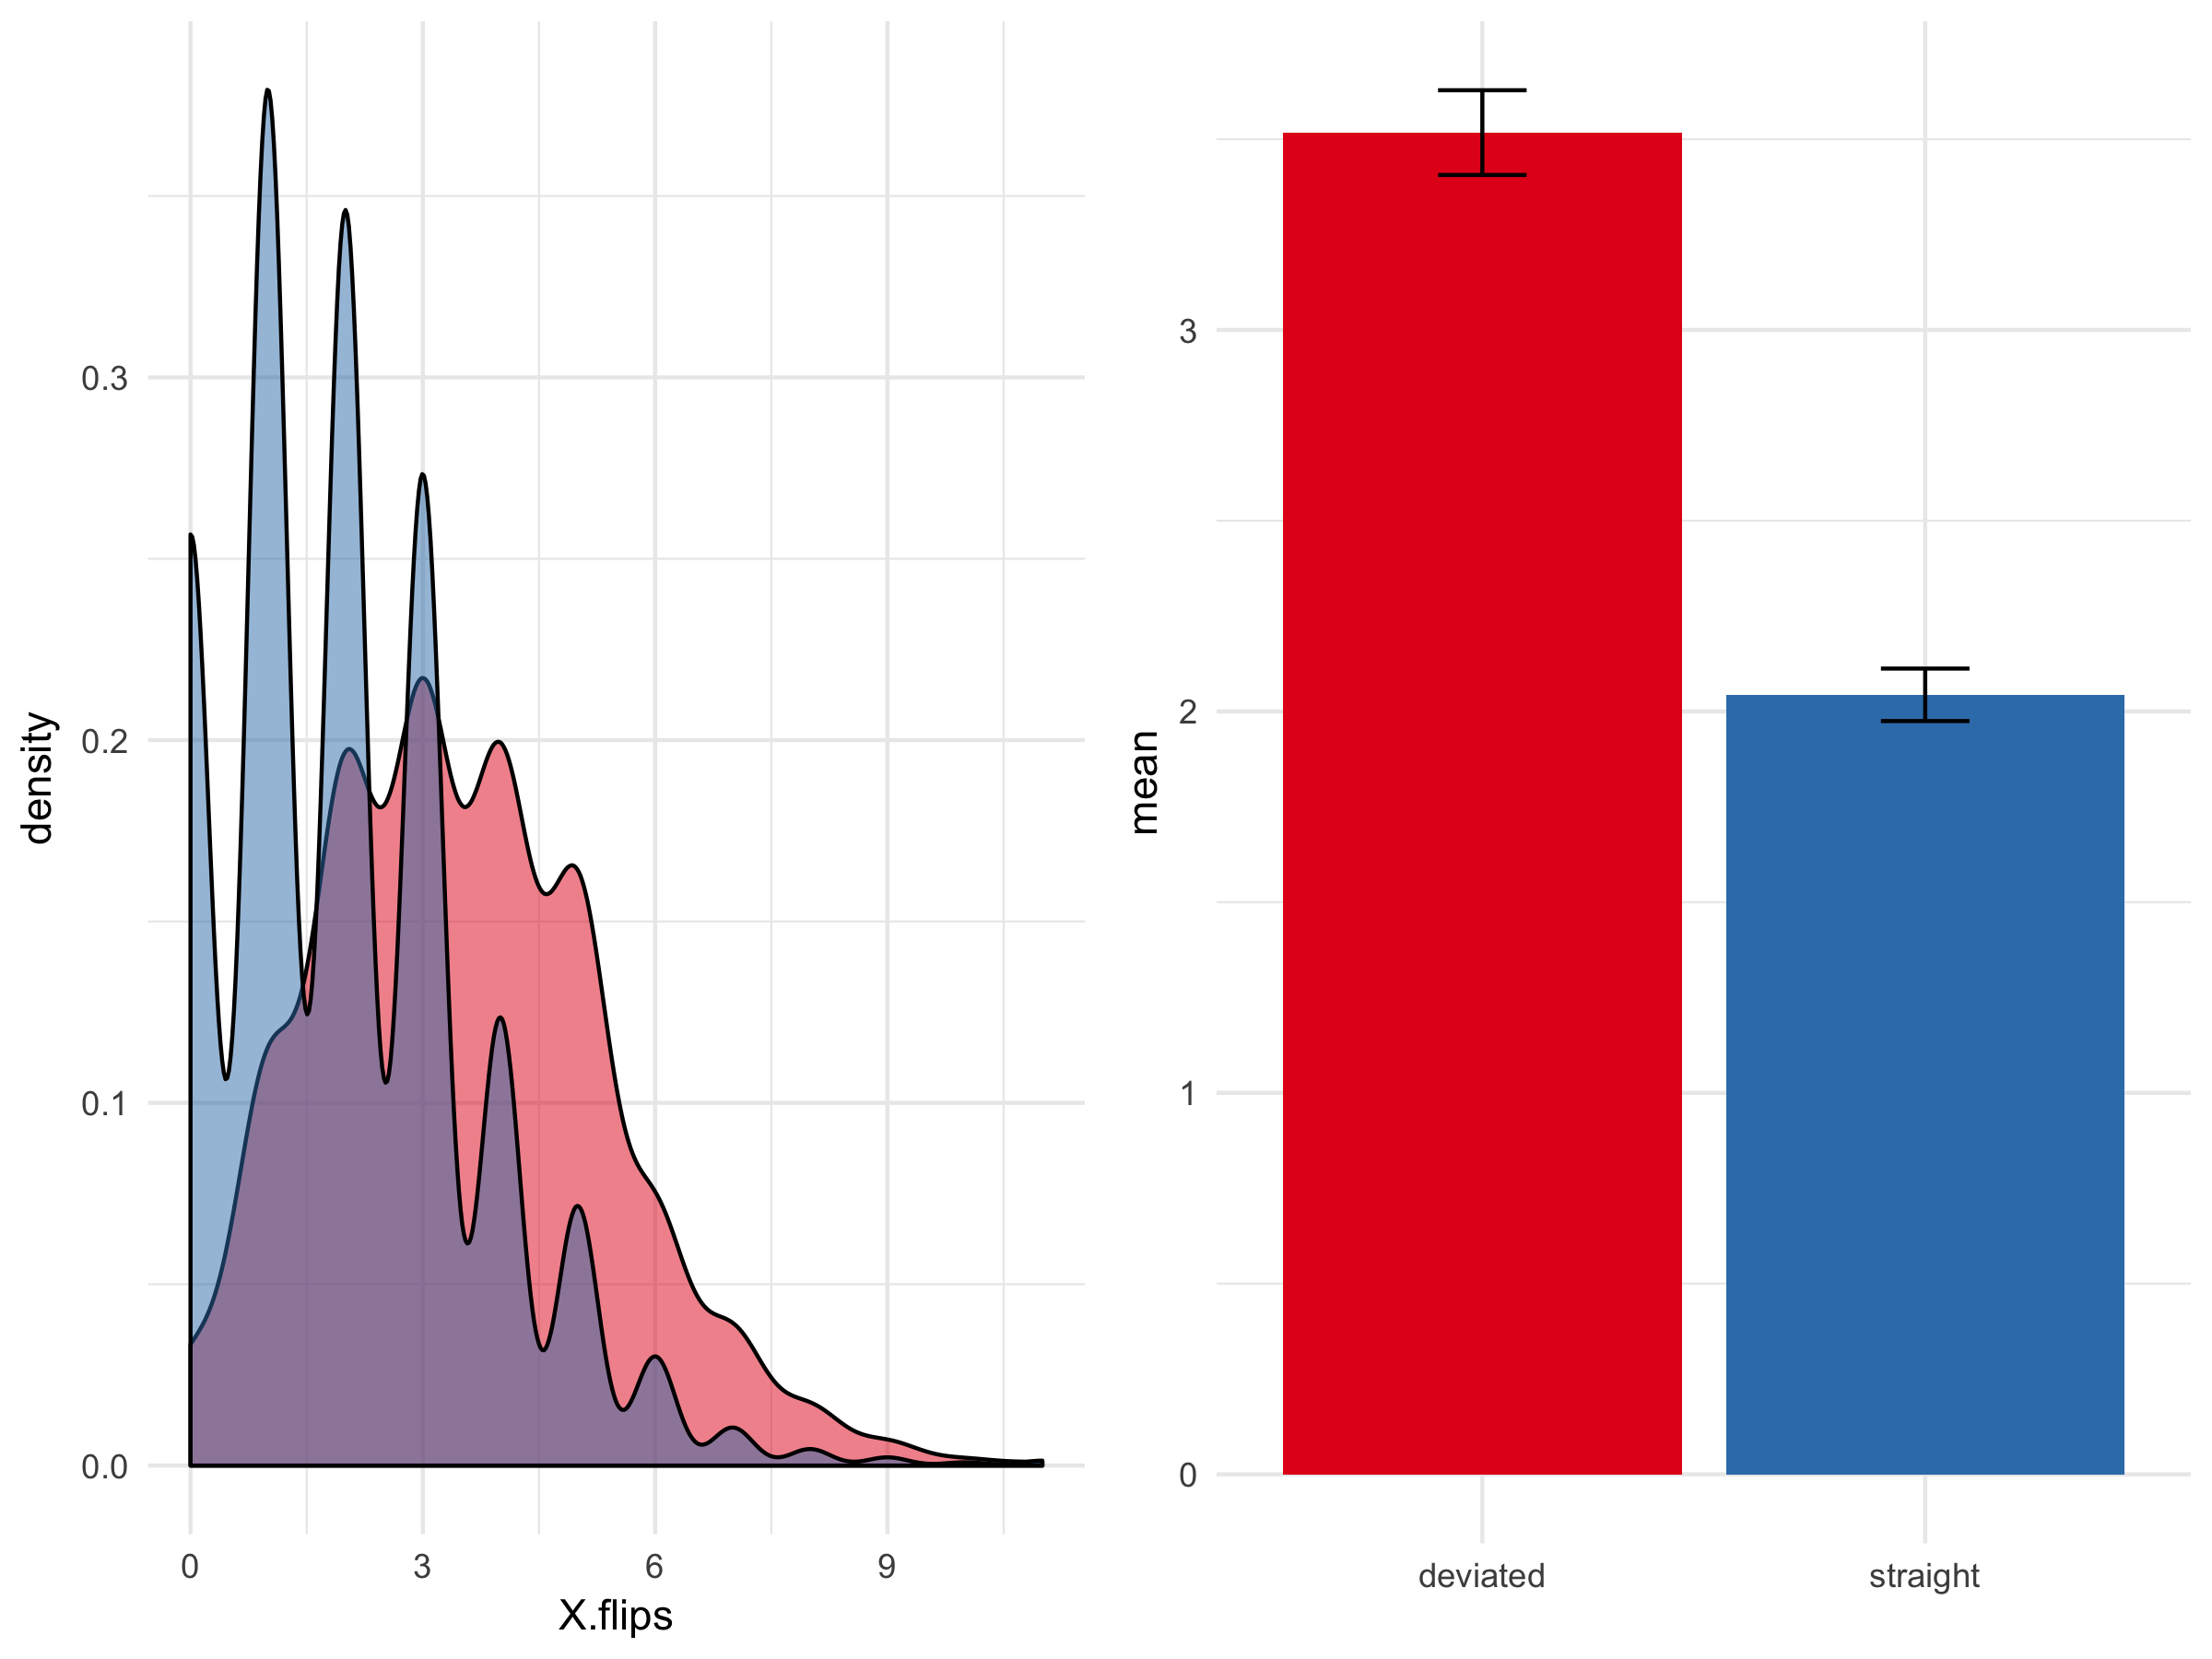
\includegraphics[width=\textwidth]{XFlips-calibration.png}
\caption{X-coordinates Flips}
\end{subfigure}
%
\begin{subfigure}[b]{0.45\textwidth}
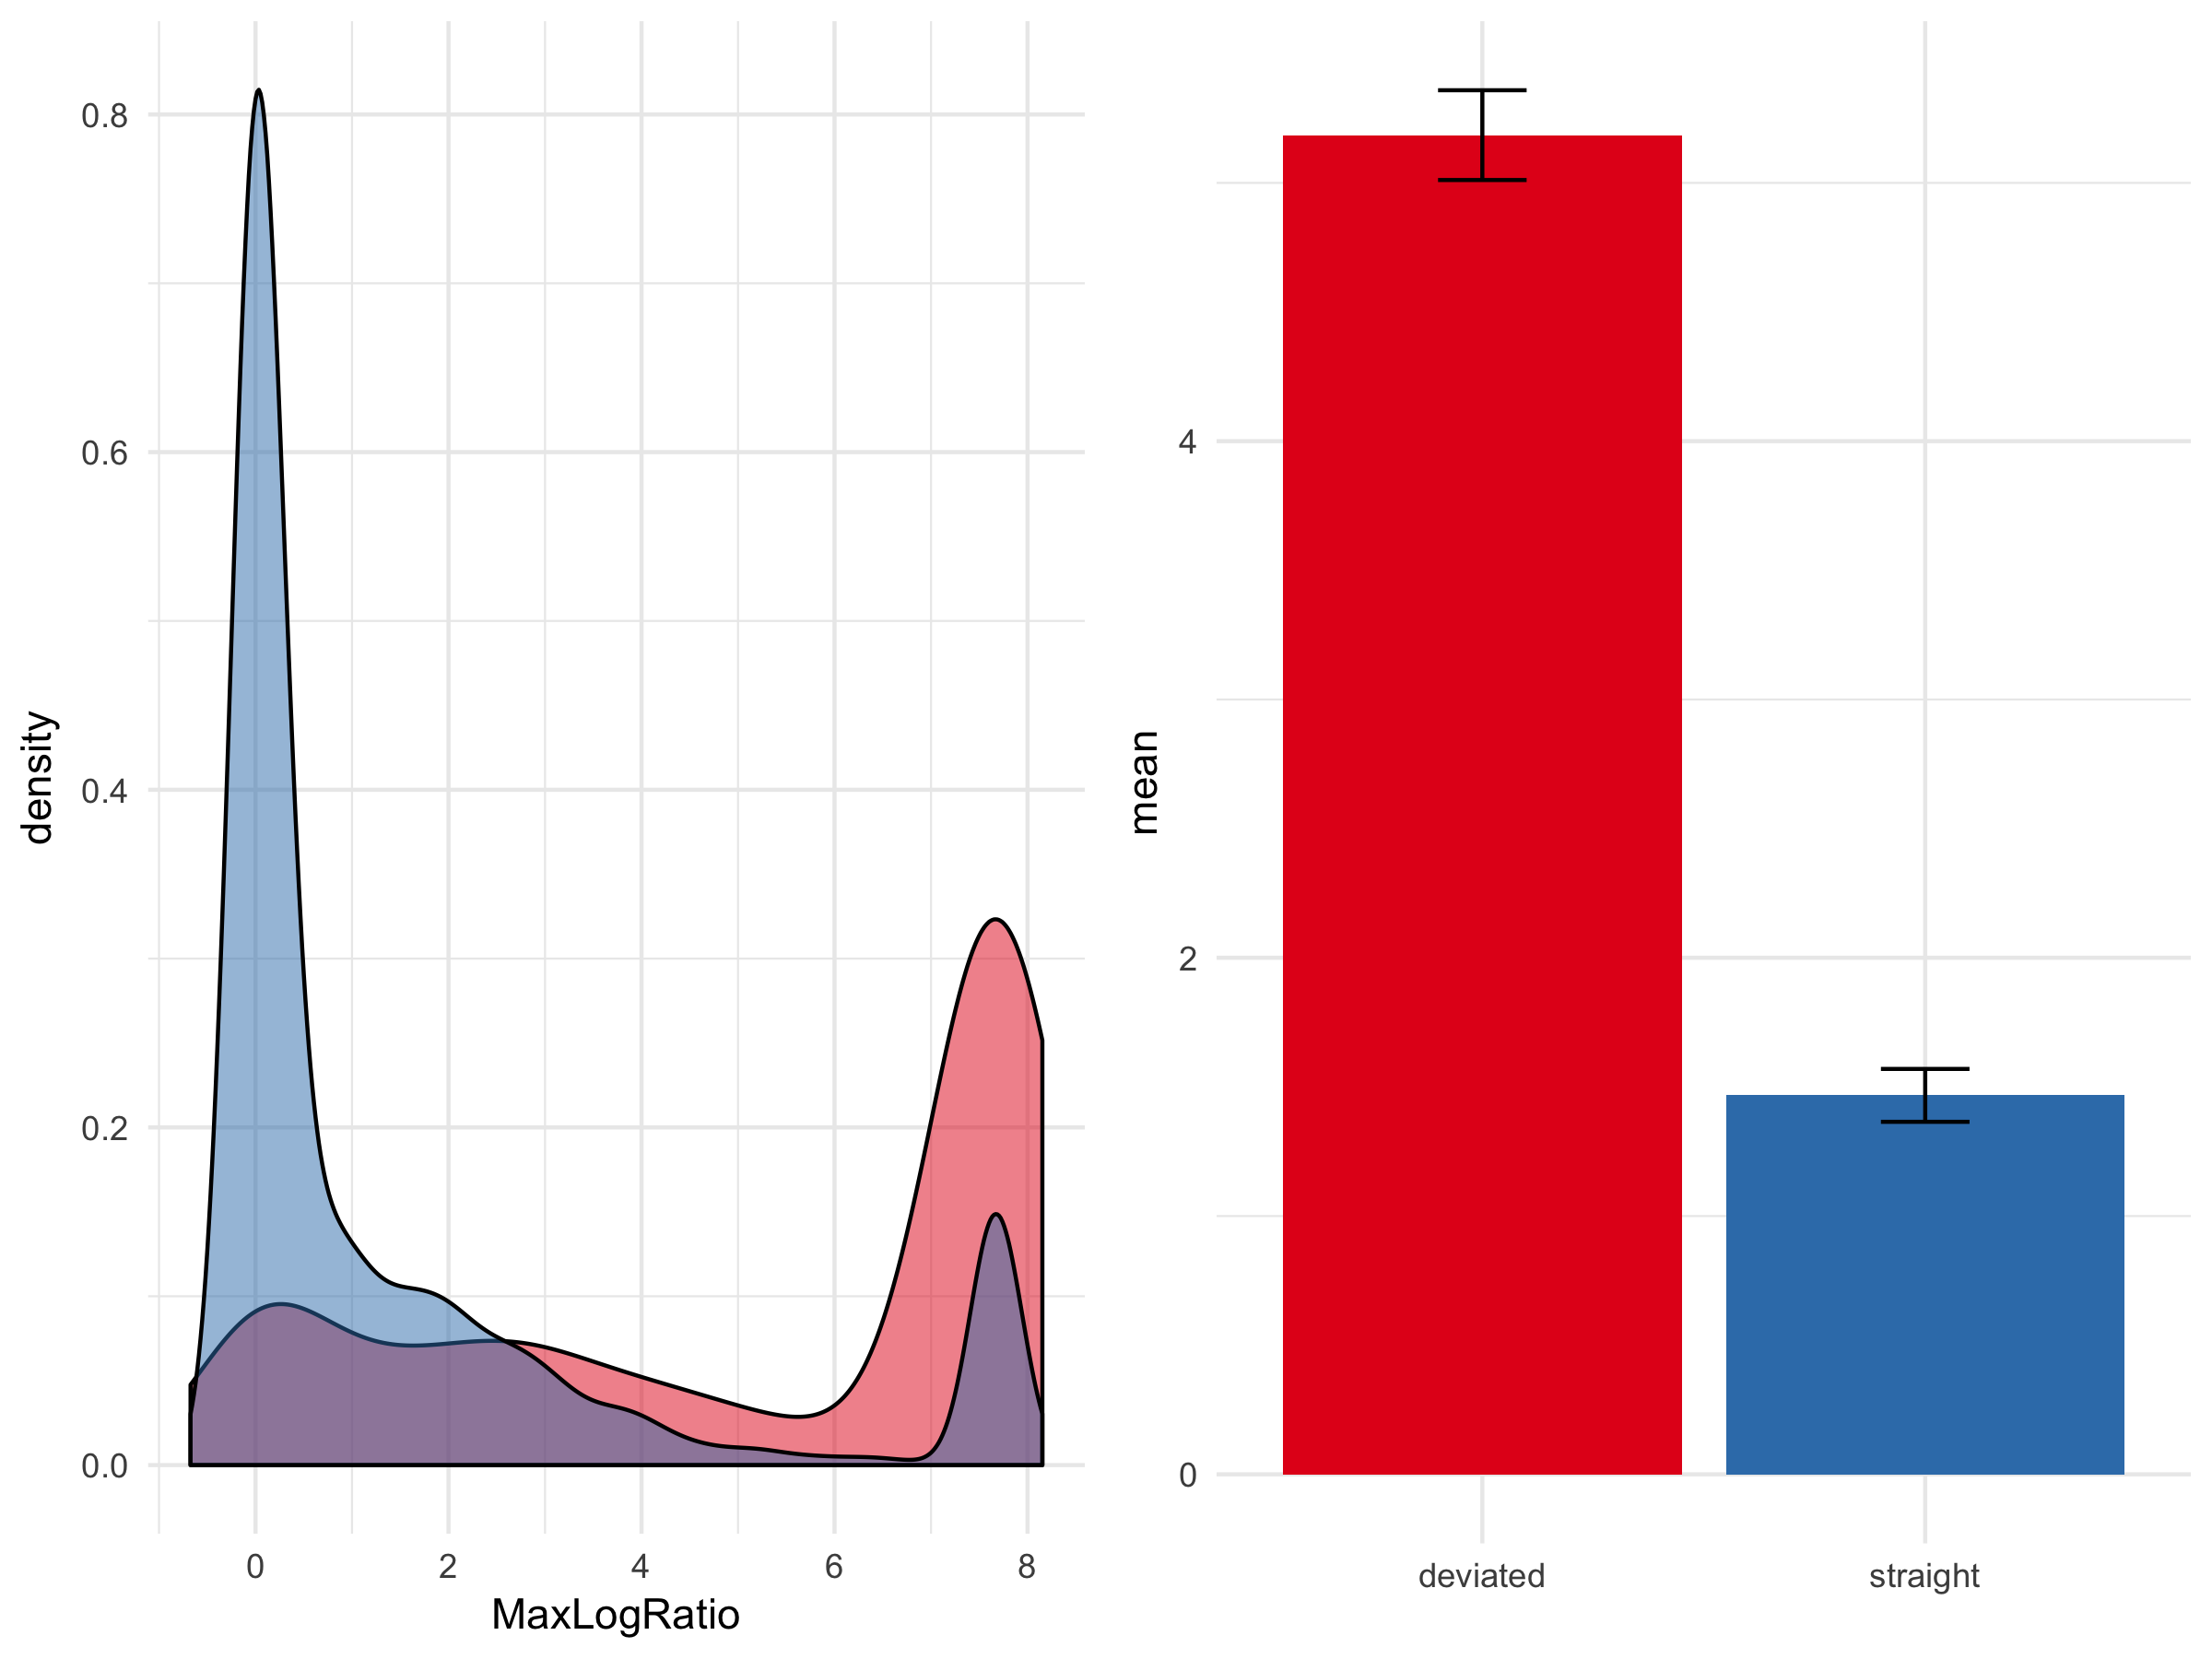
\includegraphics[width=\textwidth]{MaxLogRatio-calibration.png}
\caption{Maximal LogRatio}
\end{subfigure}

\begin{subfigure}[b]{0.45\textwidth}
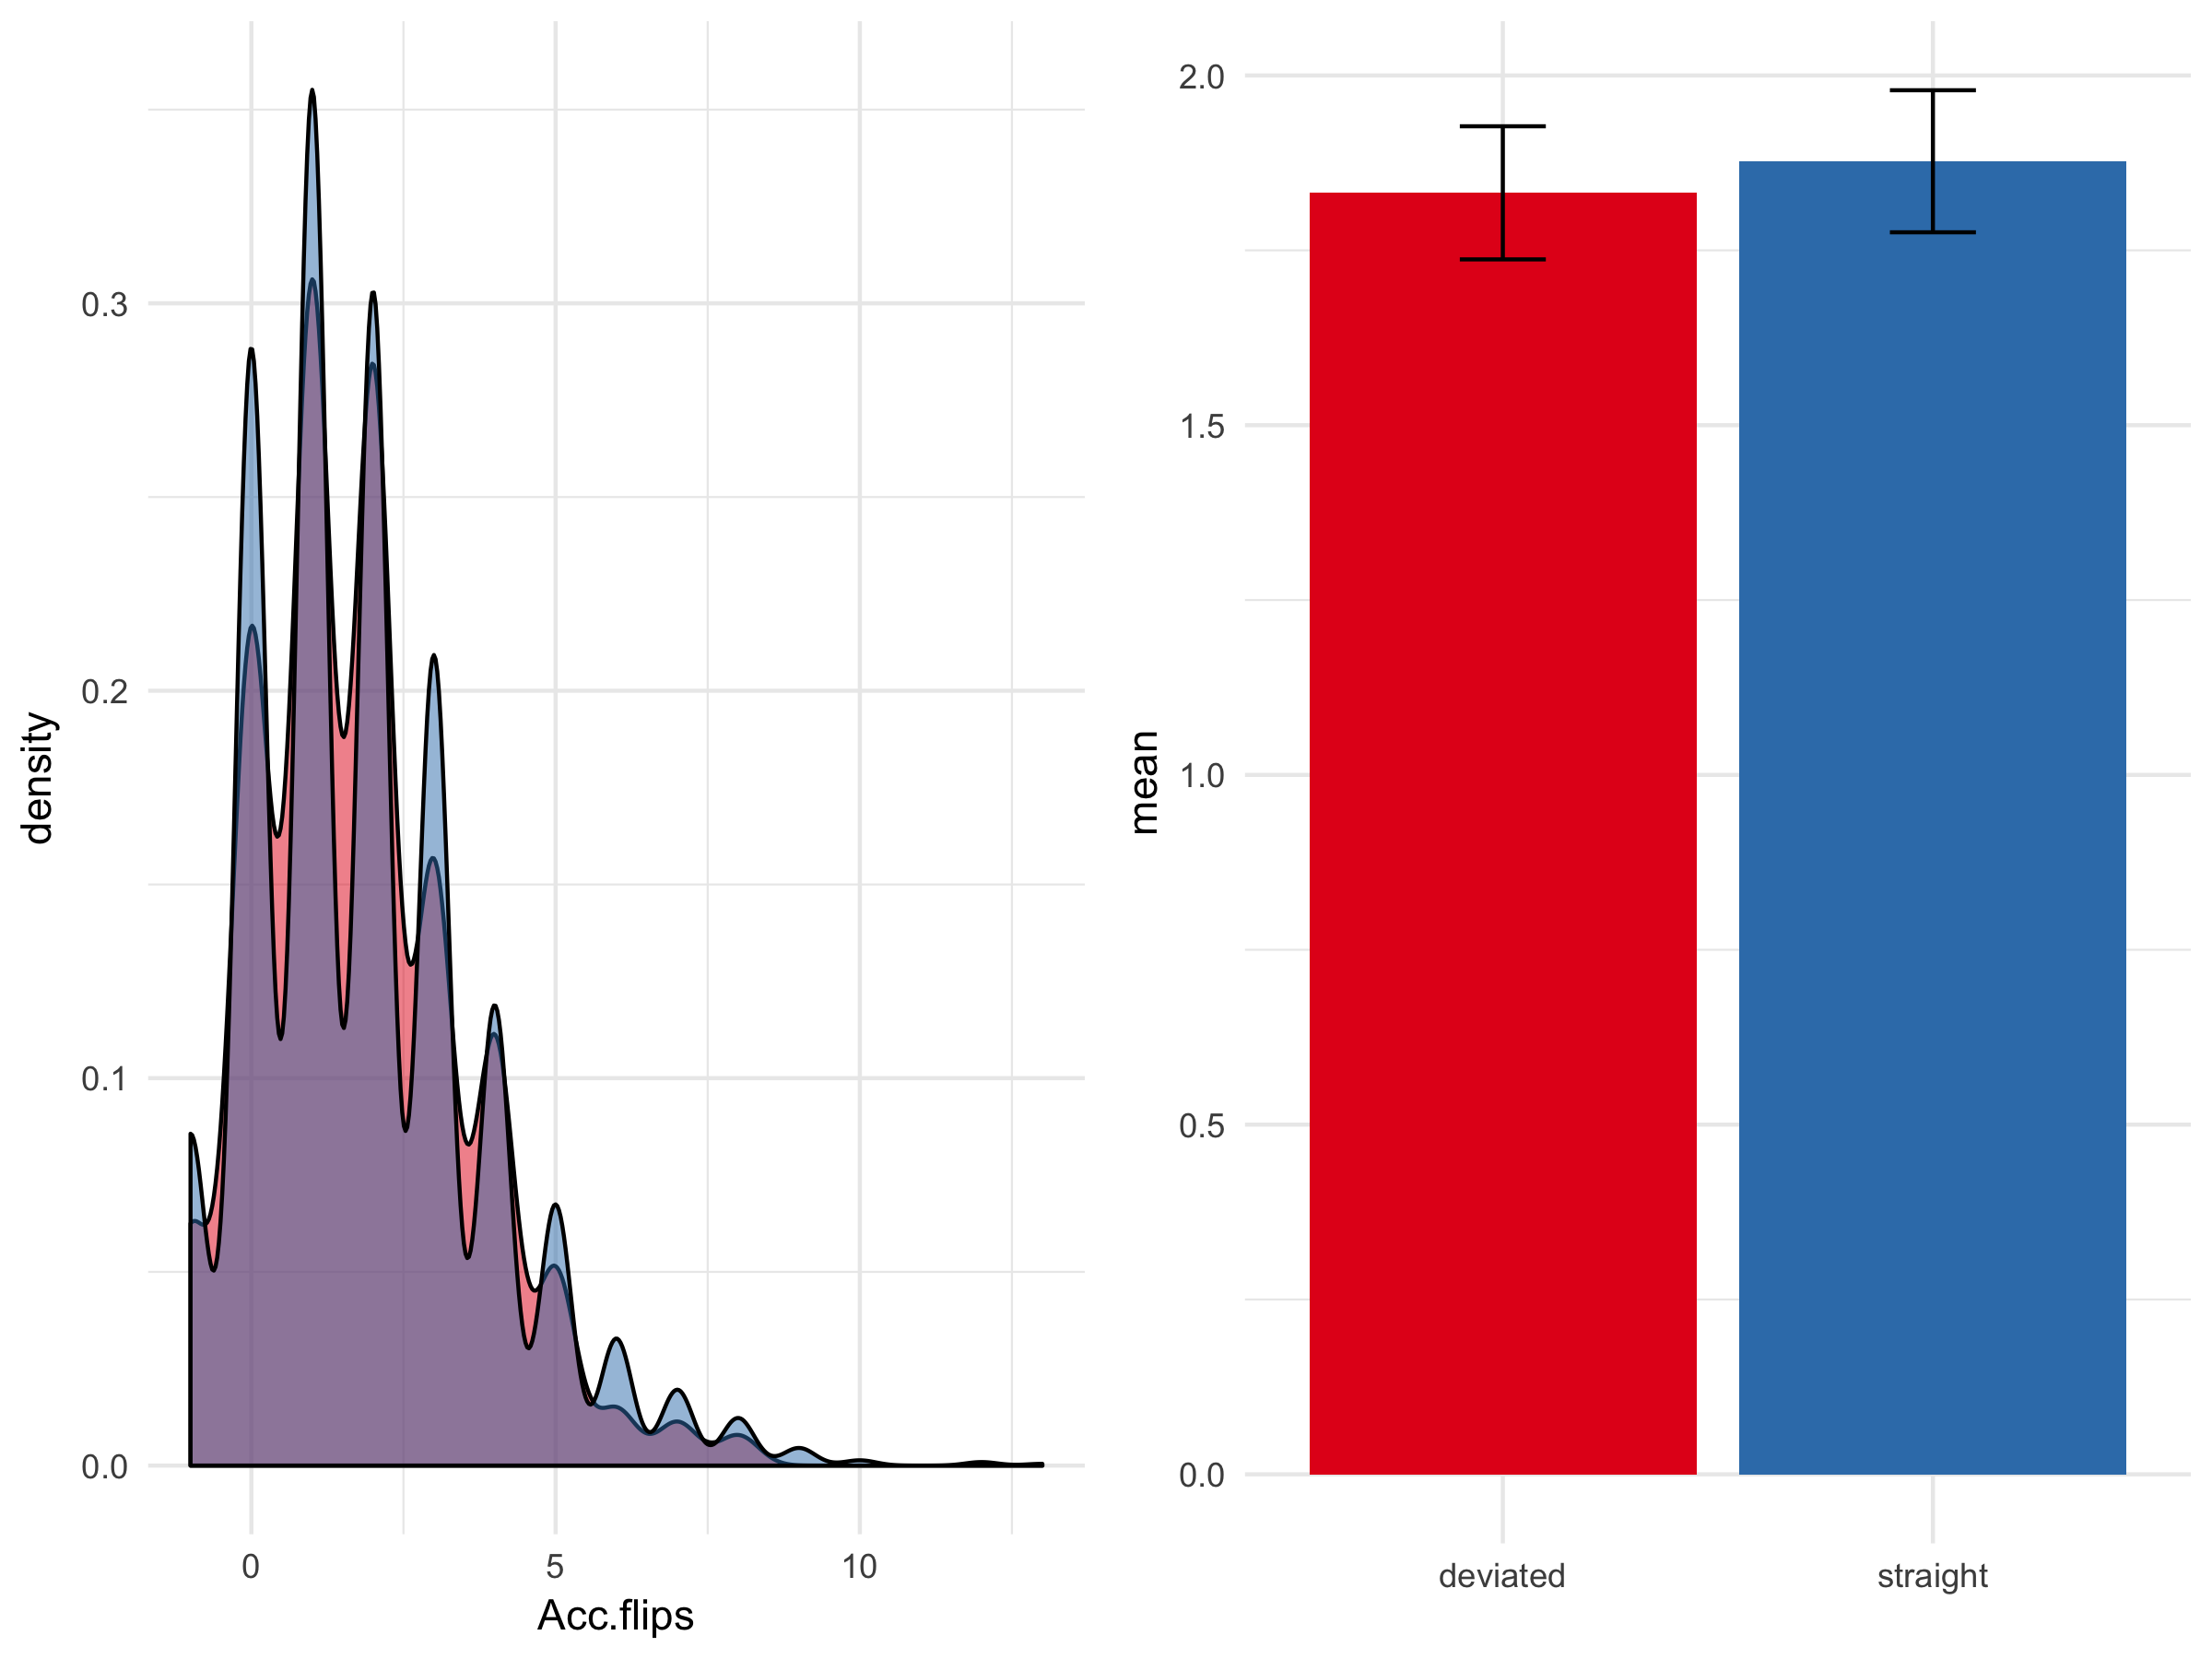
\includegraphics[width=\textwidth]{AccFlips-calibration.png}
\caption{Acceleration Flips}
\end{subfigure}

\caption{Different measures applied to our calibration data.}
\label{fig:different.measures}

\end{figure}



\item Following the cross-validation procedure described in the previous section, we diagnosed the performance of each of these measures as classifiers for our 10 bins of data. \Cref{table:comparisons.permutation.2} summarizes the results of these comparisons. 


\begin{table}[h]
\centering
\begin{tabular}{p{2cm}>{\columncolor[gray]{0.8}}p{2cm}cp{2cm}p{2cm}p{2cm}p{1.5cm}}
& \centering \textsc{Original LDA}& \textsc{AUC} & \centering \textsc{Maximal Deviation} & \centering\textsc{Maximal Log Ratio} & \centering\textsc{X-Coord. Flips} & \textsc{Acc. Flips} \\

\hline
\centering \textbf{AUC (mean)} & \centering .87 & .62 &  \centering .81 &  \centering.81 & \centering.73 & .53 \\[0.5cm]
\hline 
\centering \textbf{Mean \\ Difference} & \centering-& .24 & \centering .06 &  \centering.06  & \centering .14 & .34  \\[0.5cm]
\hline
\centering \textbf{$p$ value} &\centering - & $<$.001***& $<$.001***&$<$.001***&$<$.001***&$<$.001***\\
\hline
\end{tabular}
\caption{Cross-validation results for the LDA classifier. The performance of the LDA was compared to the one of five commonly used measures in mouse-tracking studies.}
\label{table:comparisons.permutation.2}
\end{table}


\item The results of these comparisons reveal that the LDA is significantly better at classifying our data than other commonly used measures. While the difference is in all the cases significant, the comparison between mean AUCs values suggests that measures such as Maximal Deviation and Maximal LogRatio are better at distinguishing decision processes than AUC, X and Acceleration flips. \addMM{In order to understand such pattern, it should be noticed that these two measures are the only ones that are calculated based on coordinates themselves and therefore give more importance to spatio-temporal information. In other words, both the deviation from the ideal trajectory and  the log-ratio give different weight to positions depending the moment when they occurred, and therefore are more sensitive to the moment at which deviation occurred.} 





\end{itemize}





%\multirow{''num_rows''}{''width''}{''contents''}


\section{Extension to linguistic data}

\begin{itemize}

\item Can our LDA also classify more complex decision processes, such as the ones involved in sentence verification tasks?
Dale and Duran found differences in the processing of true positive and negative sentences when people performed a simple truth-value judgement task. In this section, we aim to (1) replicate Dale \& Duran results when performing the same analyses as them, (2) to use our classifier (trained with validation data) to test these processing differences, and (3) compare the performance of our classifier with the one of other measures. 

\item Our LDA classifier is expected to dissociate between mouse trajectories that underlie a change of decision and trajectories that do not (\textit{switched} vs. \textit{straightforward}). 
If, as proposed by Dale and Duran, processing negation involves an abrupt shift in cognitive dynamics, then mouse trajectories corresponding to negative trials should pattern with trajectories involving a decision change, like the ones we included in the validation experiment. This should not be the case for trajectories corresponding to positive trials. 
If our classifier can make a distinction between negative and positive trials, we will be providing additional support to the hypothesis that, at least in this context, processing negation involves a two-step derivation (i.e. an unconscious change of decision). 

\item It should be, nevertheless, noticed that the validation data used to train the LDA is only an approximation of what should happen during an unconscious change of decision, such as the one expected for negation processing. Therefore, we expect some additional variability on the negation results (since there are some aspects of the decision process that the LDA won't be able to capture). 


\end{itemize}

\subsection{Experiment}

\begin{itemize}

\item Our experiment presented some minor methodological changes with respect to Dale and Duran's (Experiment 1), but it tested the same contrast; namely, the interaction between truth value (true or false statements) and sentence polarity (affirmative and negative sentences). 

\item Participants were asked to perform a truth-judgment task, where they had decide whether a statement is true or false according to common knowledge. 

\item Unlike Dale and Duran's experiment, the complete statement was presented in the middle of the screen after participants pressed ``Start" (i.e. no self-paced reading). The ``True" and ``False"  boxes appear at the top-left or top-right corners of the screen, in the same way as in our validation experiment.  

\item Each of the sentences could be either a true or a false statement in its negated or non-negated form. 
An illustration of the sentences used as examples is provided in \Cref{table:exampleDD}. 


\end{itemize}

\paragraph{Participants}
53 English native speakers were tested using Amazon Mechanical Turk. They were rewarded for their participation.  

\paragraph{Design}
The experimental design consisted in two fully crossed factors: \textsc{Truth} (true, false) and \textsc{Polarity} (negative, positive). We had a total of 4 conditions, and each participant saw 4 instances of each condition (16 sentences). 


\begin{figure}
\centering
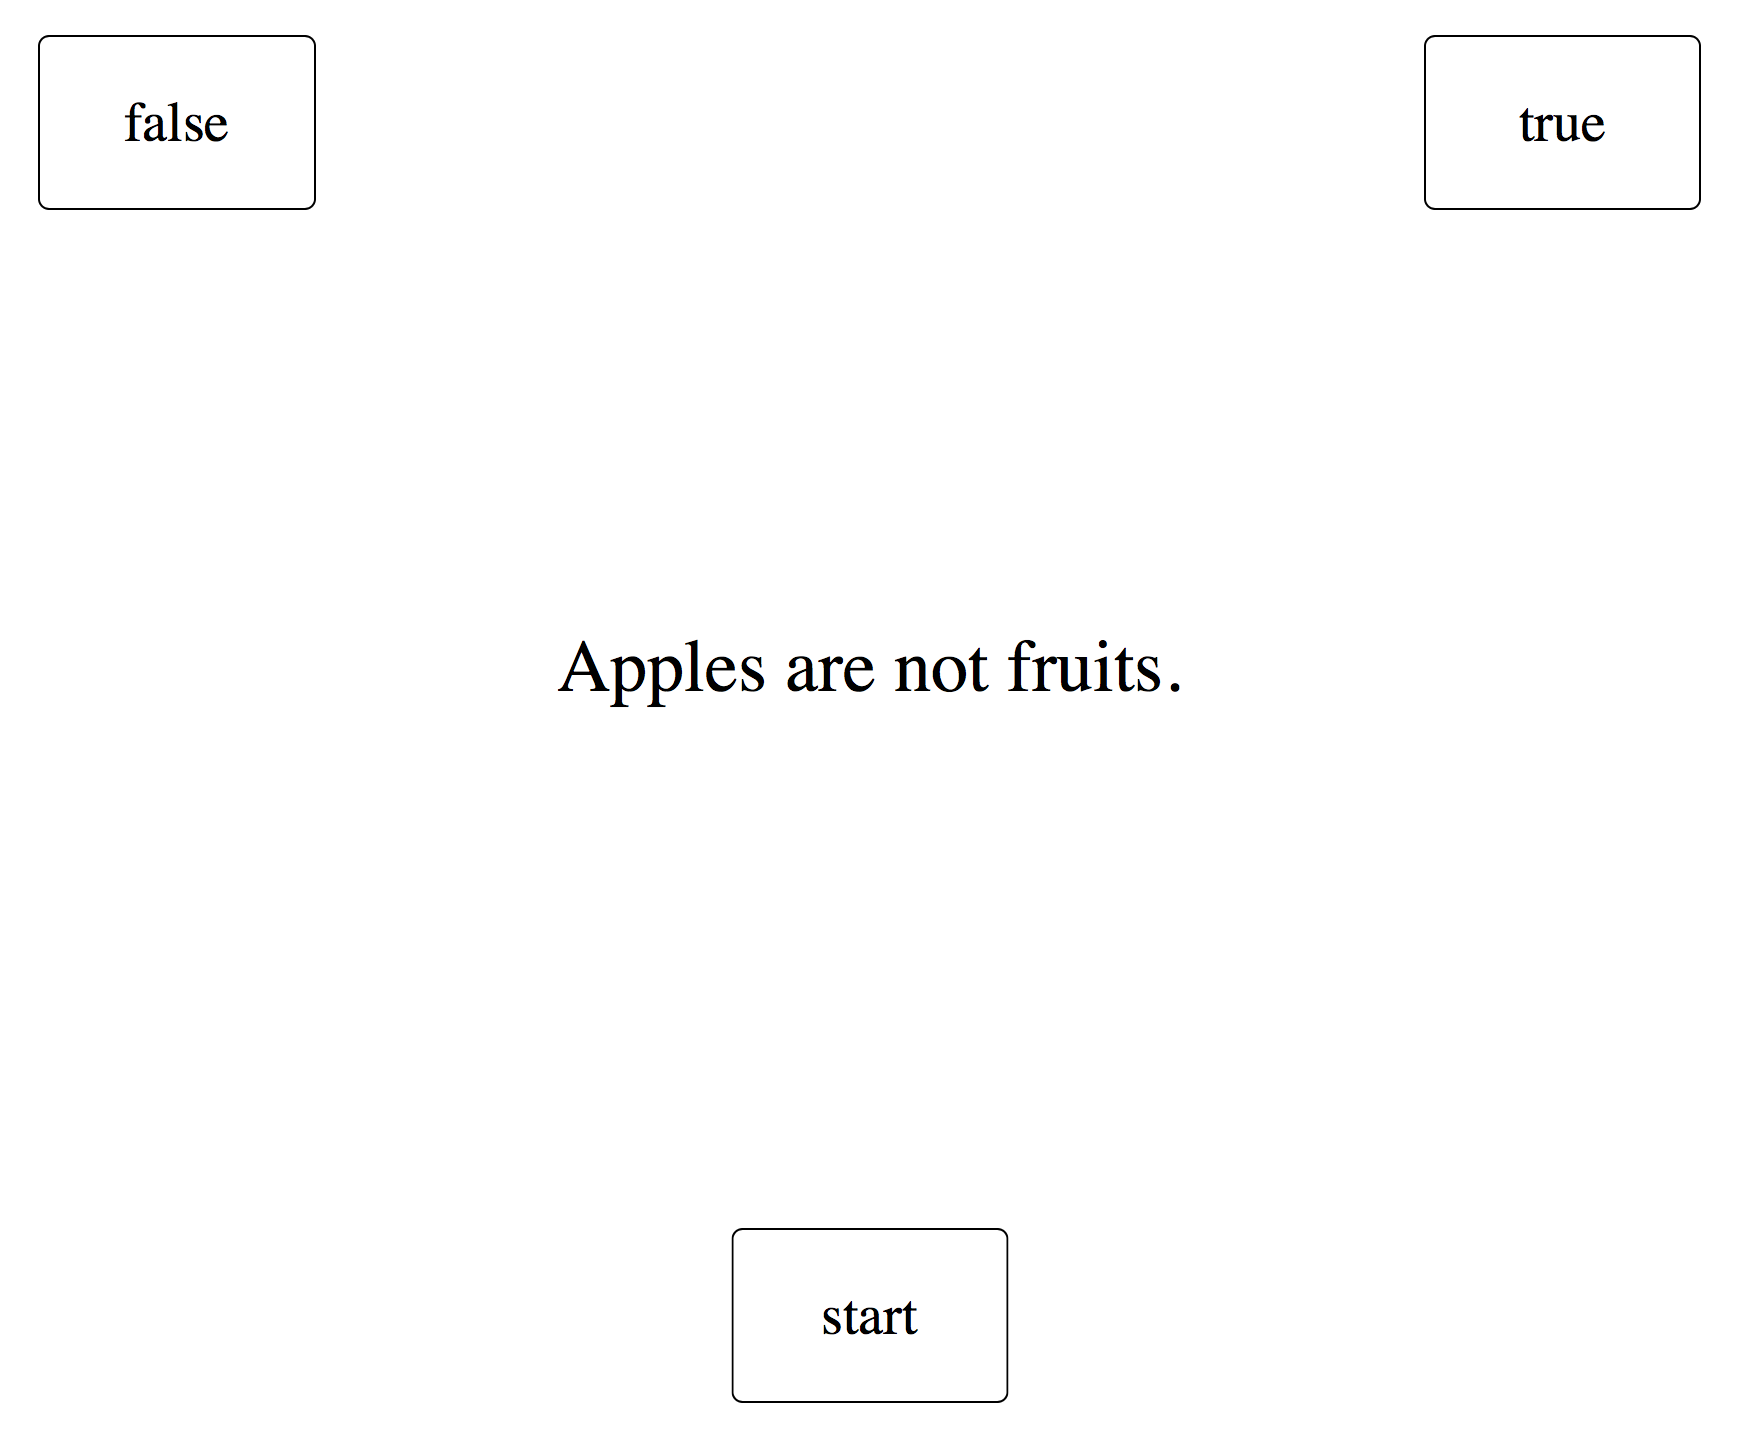
\includegraphics[width=0.7\textwidth]{trial_example2.png}
\caption{Trial Example Dale \& Duran Replication}
\end{figure}



\begin{table}[h]
\centering
\begin{tabular}{ccc}
Truth value & Polarity & Example \\
\hline
\multirow{2}{*}{True} & Positive & Cars have wheels.\\ 
 & Negatives & Cars have no wings.\\ 
\hline
\multirow{2}{*}{False} & Positive & Cars have wings.\\ 
 & Negatives & Cars have no wheels.\\
\end{tabular}
\caption{Design} \label{table:exampleDD}
\end{table}


\paragraph{Interface and data treatment}
The interface and data treatment were the same as the ones used for the calibration experiment. Mouse trajectories' time course was normalised into 101 time steps.

\subsection{Results}
\paragraph{Replicating Dale and Duran (2011)}

\begin{itemize}
\item All participants responded correctly more than 75\% of the time. No participant was discarded based on accuracy.  Only accurate trials were taken into account for the analysis. Mean trajectories for the four possible trial conditions are shown in \Cref{fig:mean.trajectory-negation}. 

\begin{figure}
\centering
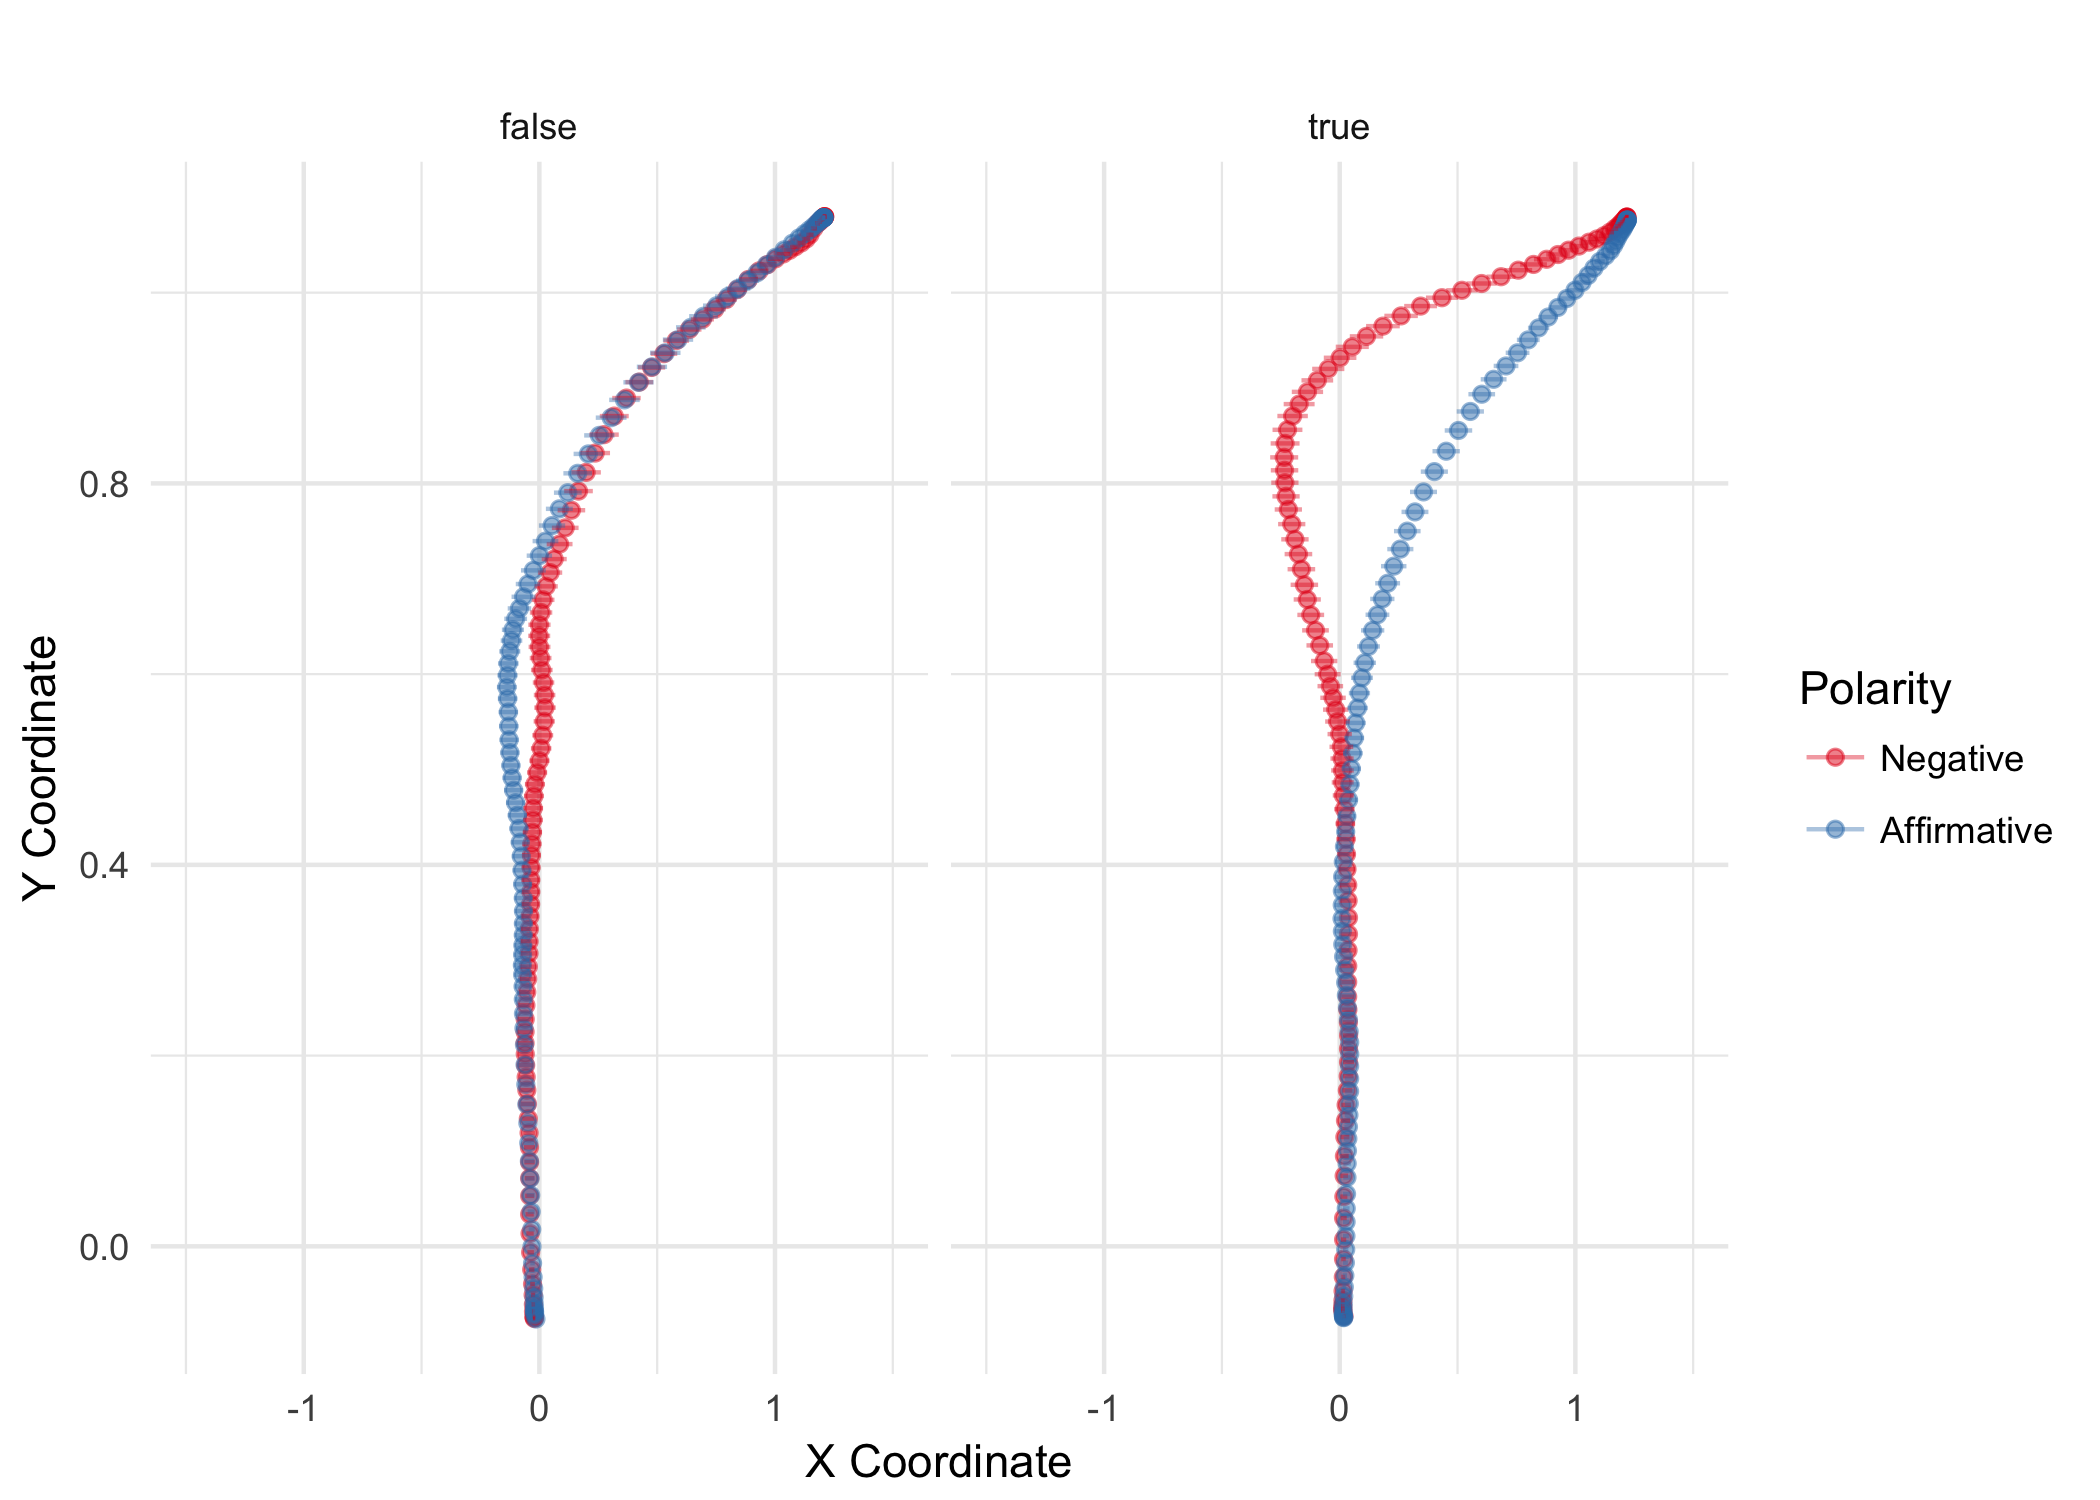
\includegraphics[width=0.7\textwidth]{negation-data-mean-trajectory.png}
\caption{Mean trajectories for accurate trials} \label{fig:mean.trajectory-negation}
\end{figure}

\item To assess whether we replicate Dale and Duran's results, we calculated the $x$-flips (see above) and analysed them with a linear mixed-effects model (Baayen, Davidson, and Bates, 2008), taking Truth, Polarity and their interaction as predictors. We included random intercepts per subject and a random slope with the interaction of both factors. $P$-values were obtained by comparing the omnibus model to a reduced version of itself, where the relevant factor was removed. This pipeline mirrors the model performed by D\&D. 

\item Unlike Dale and Duran, we did not perform analyses based on the acceleration component (acceleration flips). Our validation experiment suggest that this measure is unable to dissociate trajectories involving a change of decision from straight trajectories. This seems to be related with the fact that our data is very noisy. 
We reasoned that if the different decision processes involved in a rather simple task were not captured by the acceleration component, this measure would also be unable to classify more complex processes, such as the ones at play in a sentence verification task. 

\item The model revealed a main effect of Polarity, such that negation significantly increases $x$-flips by 0.76 ($\chi^{2}=10.11; p=.0014$), and a significant interaction Truth $\times$ Polarity ($\chi^{2}=22.7; p<.001$), such that the difference between negative and positive sentence is bigger for the true than for the false statements. There was no significant effect of Truth ($\chi^{2}<1; p=.5$). 
\Cref{table:negationresults} summarises the pattern of means and estimates for both ours and Dale and Duran's results. 

\begin{table}[h]
\caption{default}
\begin{center}
\begin{tabular}{ccc}
Condition & $x$-flips &  $x$-flips in D\&D \\
\hline
T/no negation & 2.22 & 1.13 \\
T/negation & 3.67 & 1.71 \\
F/no negation & 2.82 & 1.24 \\
F/negation & 2.9 & 1.34 \\
Estimate Polarity & .76 & 0.35 \\
Estimate Truth & .07 & 0.13 \\
Estimate Truth$\times$Polarity & 1.35 & 0.47\\
\end{tabular}
\caption{Mean and effect estimates}
\label{table:negationresults}
\end{center}
\label{default}
\end{table}%

\item These results seem to replicate Dale and Duran's findings: verifying true negated sentences produces less straightforward trajectories than true positive sentences. It should, however, be noticed that the values obtained in the two experiments are slightly different; namely, our results present higher range of values. As for the acceleration component, this might be due to the fact that our data is generally noisier than theirs, probably because of $x,y$ coordinates were sampled from mouse-movements and not at a fixed sampling rate.

\item More generally, our findings pattern with a broader set of psycholinguistic studies, which have used different techniques and shown that verifying negative sentences involve computing the positive content at an early processing stage (CITE). 


\end{itemize}

\paragraph{Classifier performance}
\begin{itemize}

\item Two different LDA classifiers, trained with validation data, were applied to the new experimental data. The first classifier was our original LDA, which had as predictors $x,y$ coordinates as well as velocity and acceleration. The second LDA had only $x,y$ coordinates as predictors. Validation results (see above) suggest that the simpler model, which only relies on coordinates information, might be sufficient to classify the data. In other words, the simple model might fit the data as well as a more complex model, and be interpreted more straightforwardly. 

\item Since the relevant different between the positive and negative sentences is expected to arise specifically for \emph{true} statements, we will analyse specifically these cases (NB: This will facilitate the analyses).  

\item Distribution and means of the resulting \textit{LDA measure} for \emph{true} trials and for both classifiers are illustrated in \Cref{fig:lda_negation}. As before, the overall performance of the classifier was evaluated by calculating the area under the ROC curve (Original LDA=.7; Coords LDA=.66). \addMM{Add LMM for these measures?}

\begin{figure}
\centering
\begin{subfigure}[b]{0.45\textwidth}
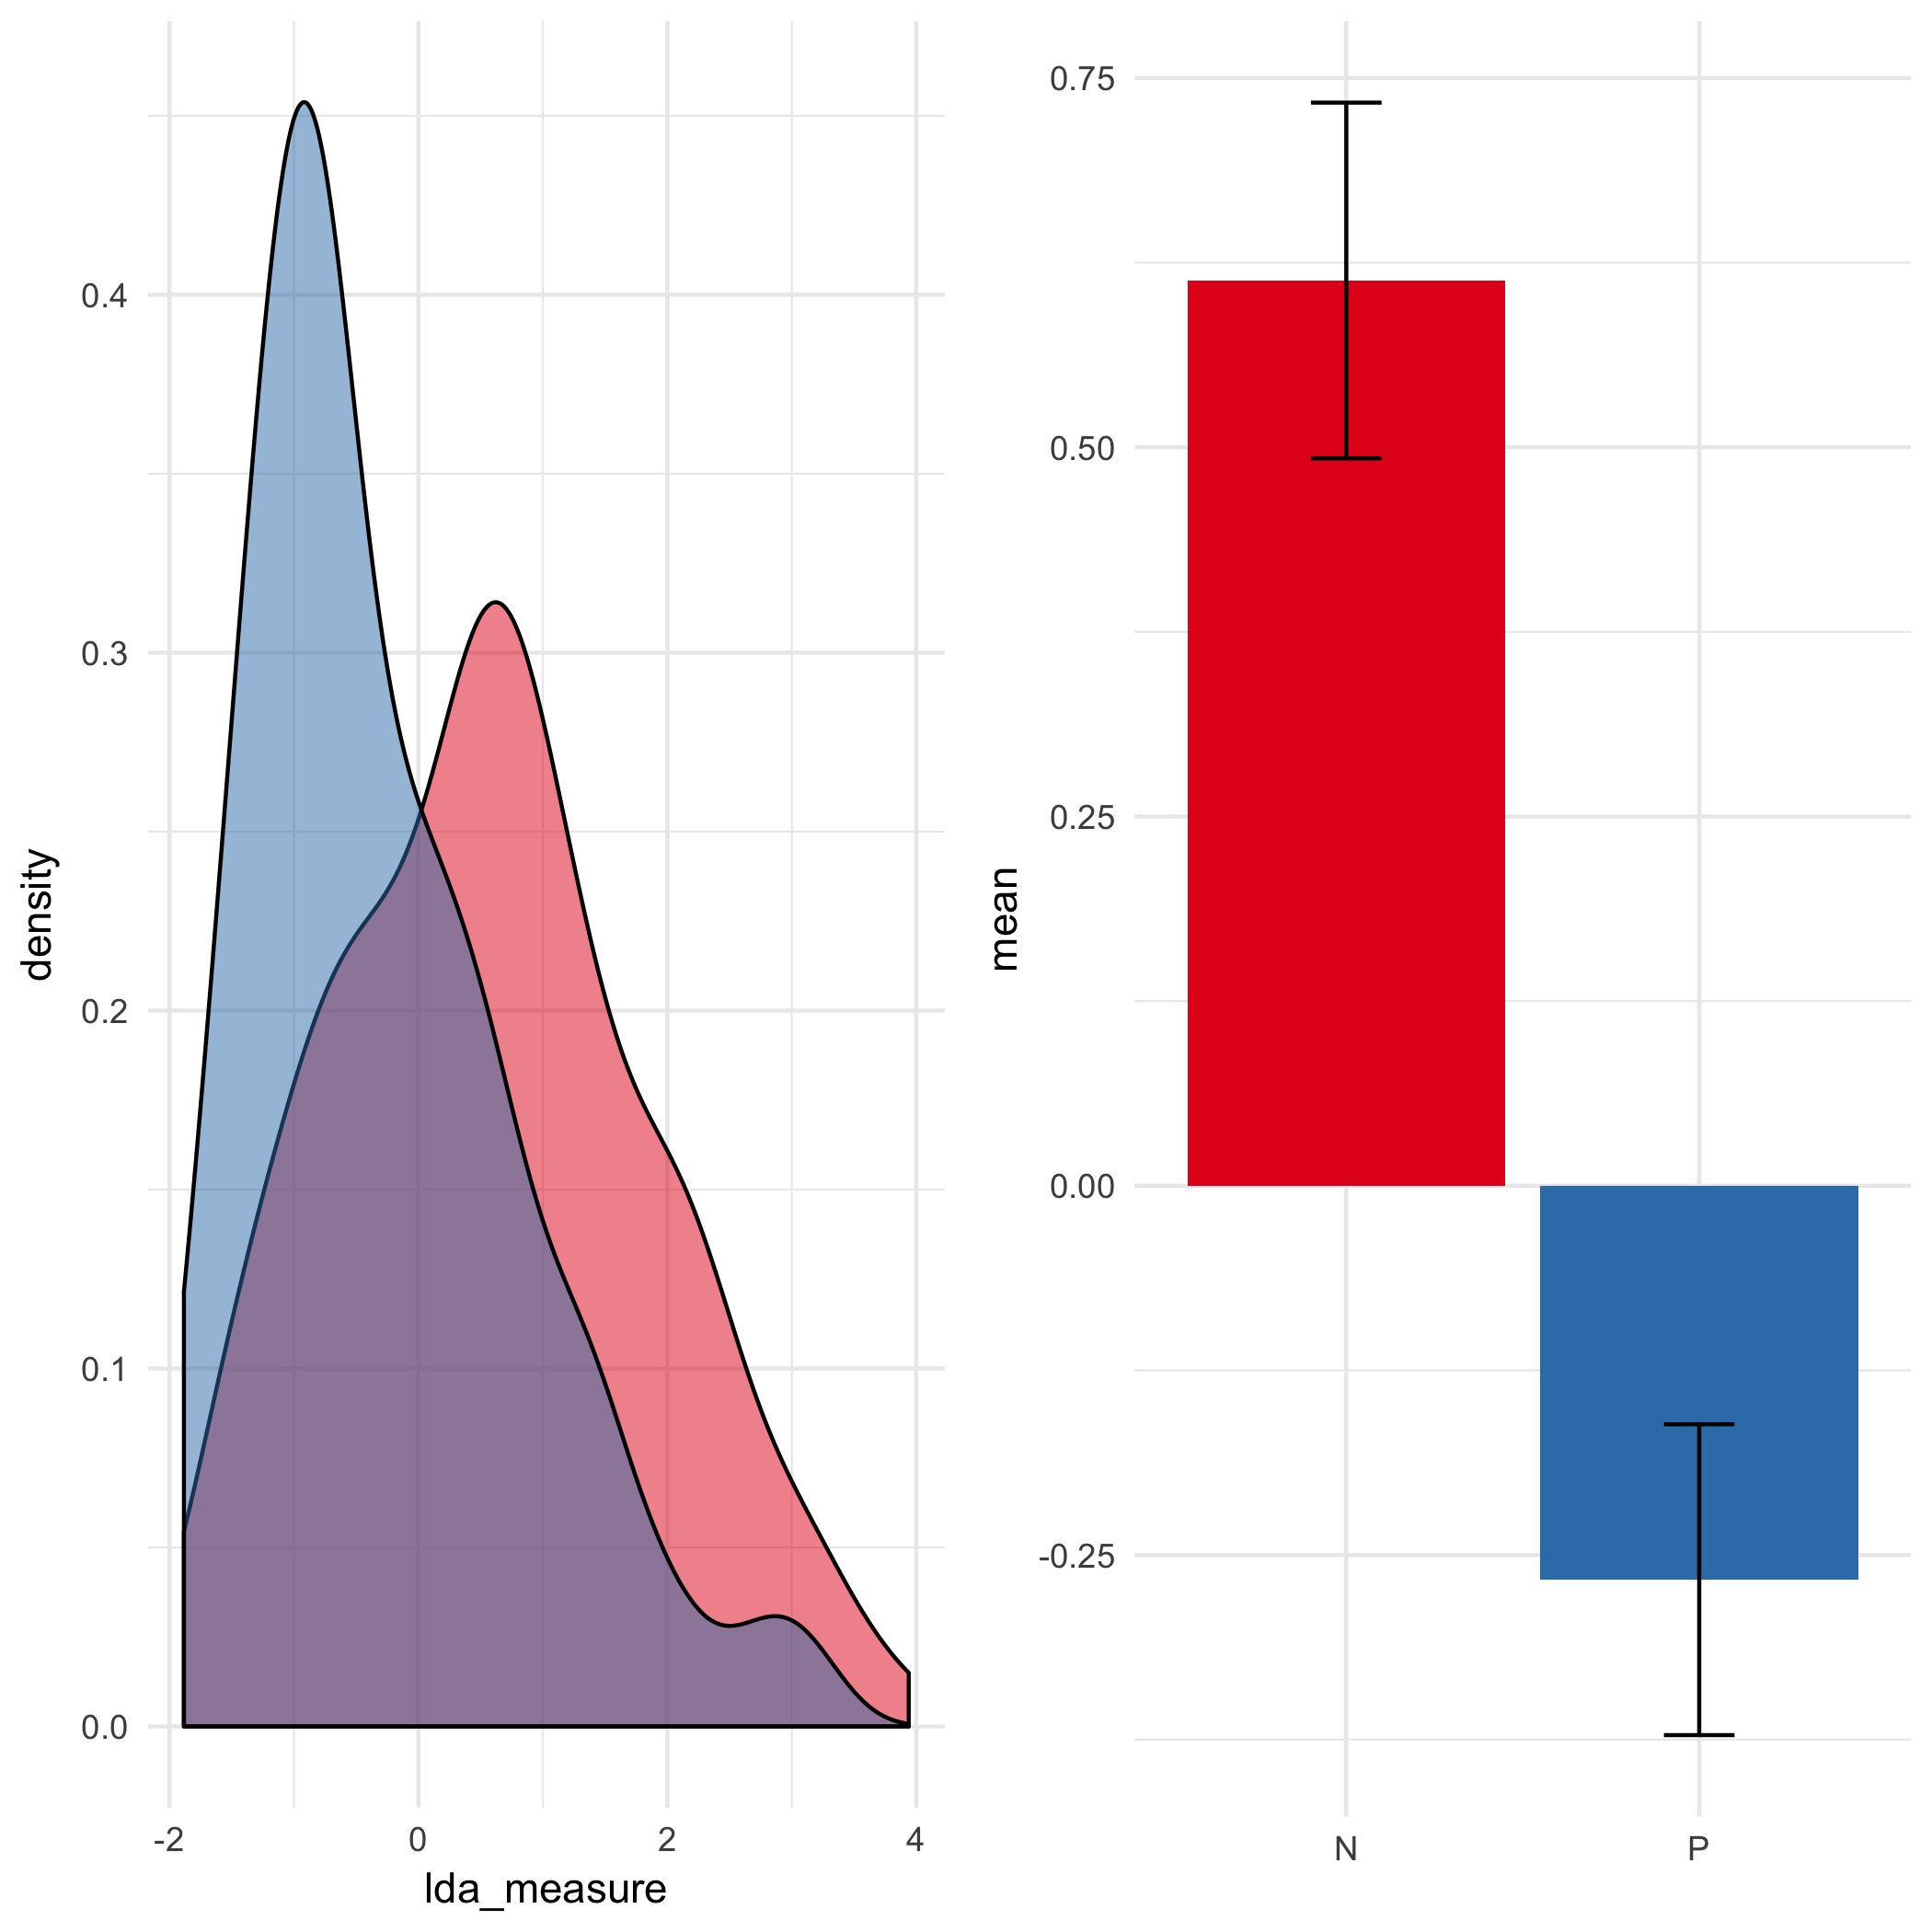
\includegraphics[width=\textwidth]{LDA-negation.png}
\caption{Original LDA (coords, speed and acceleration) }
\end{subfigure}
\begin{subfigure}[b]{0.45\textwidth}
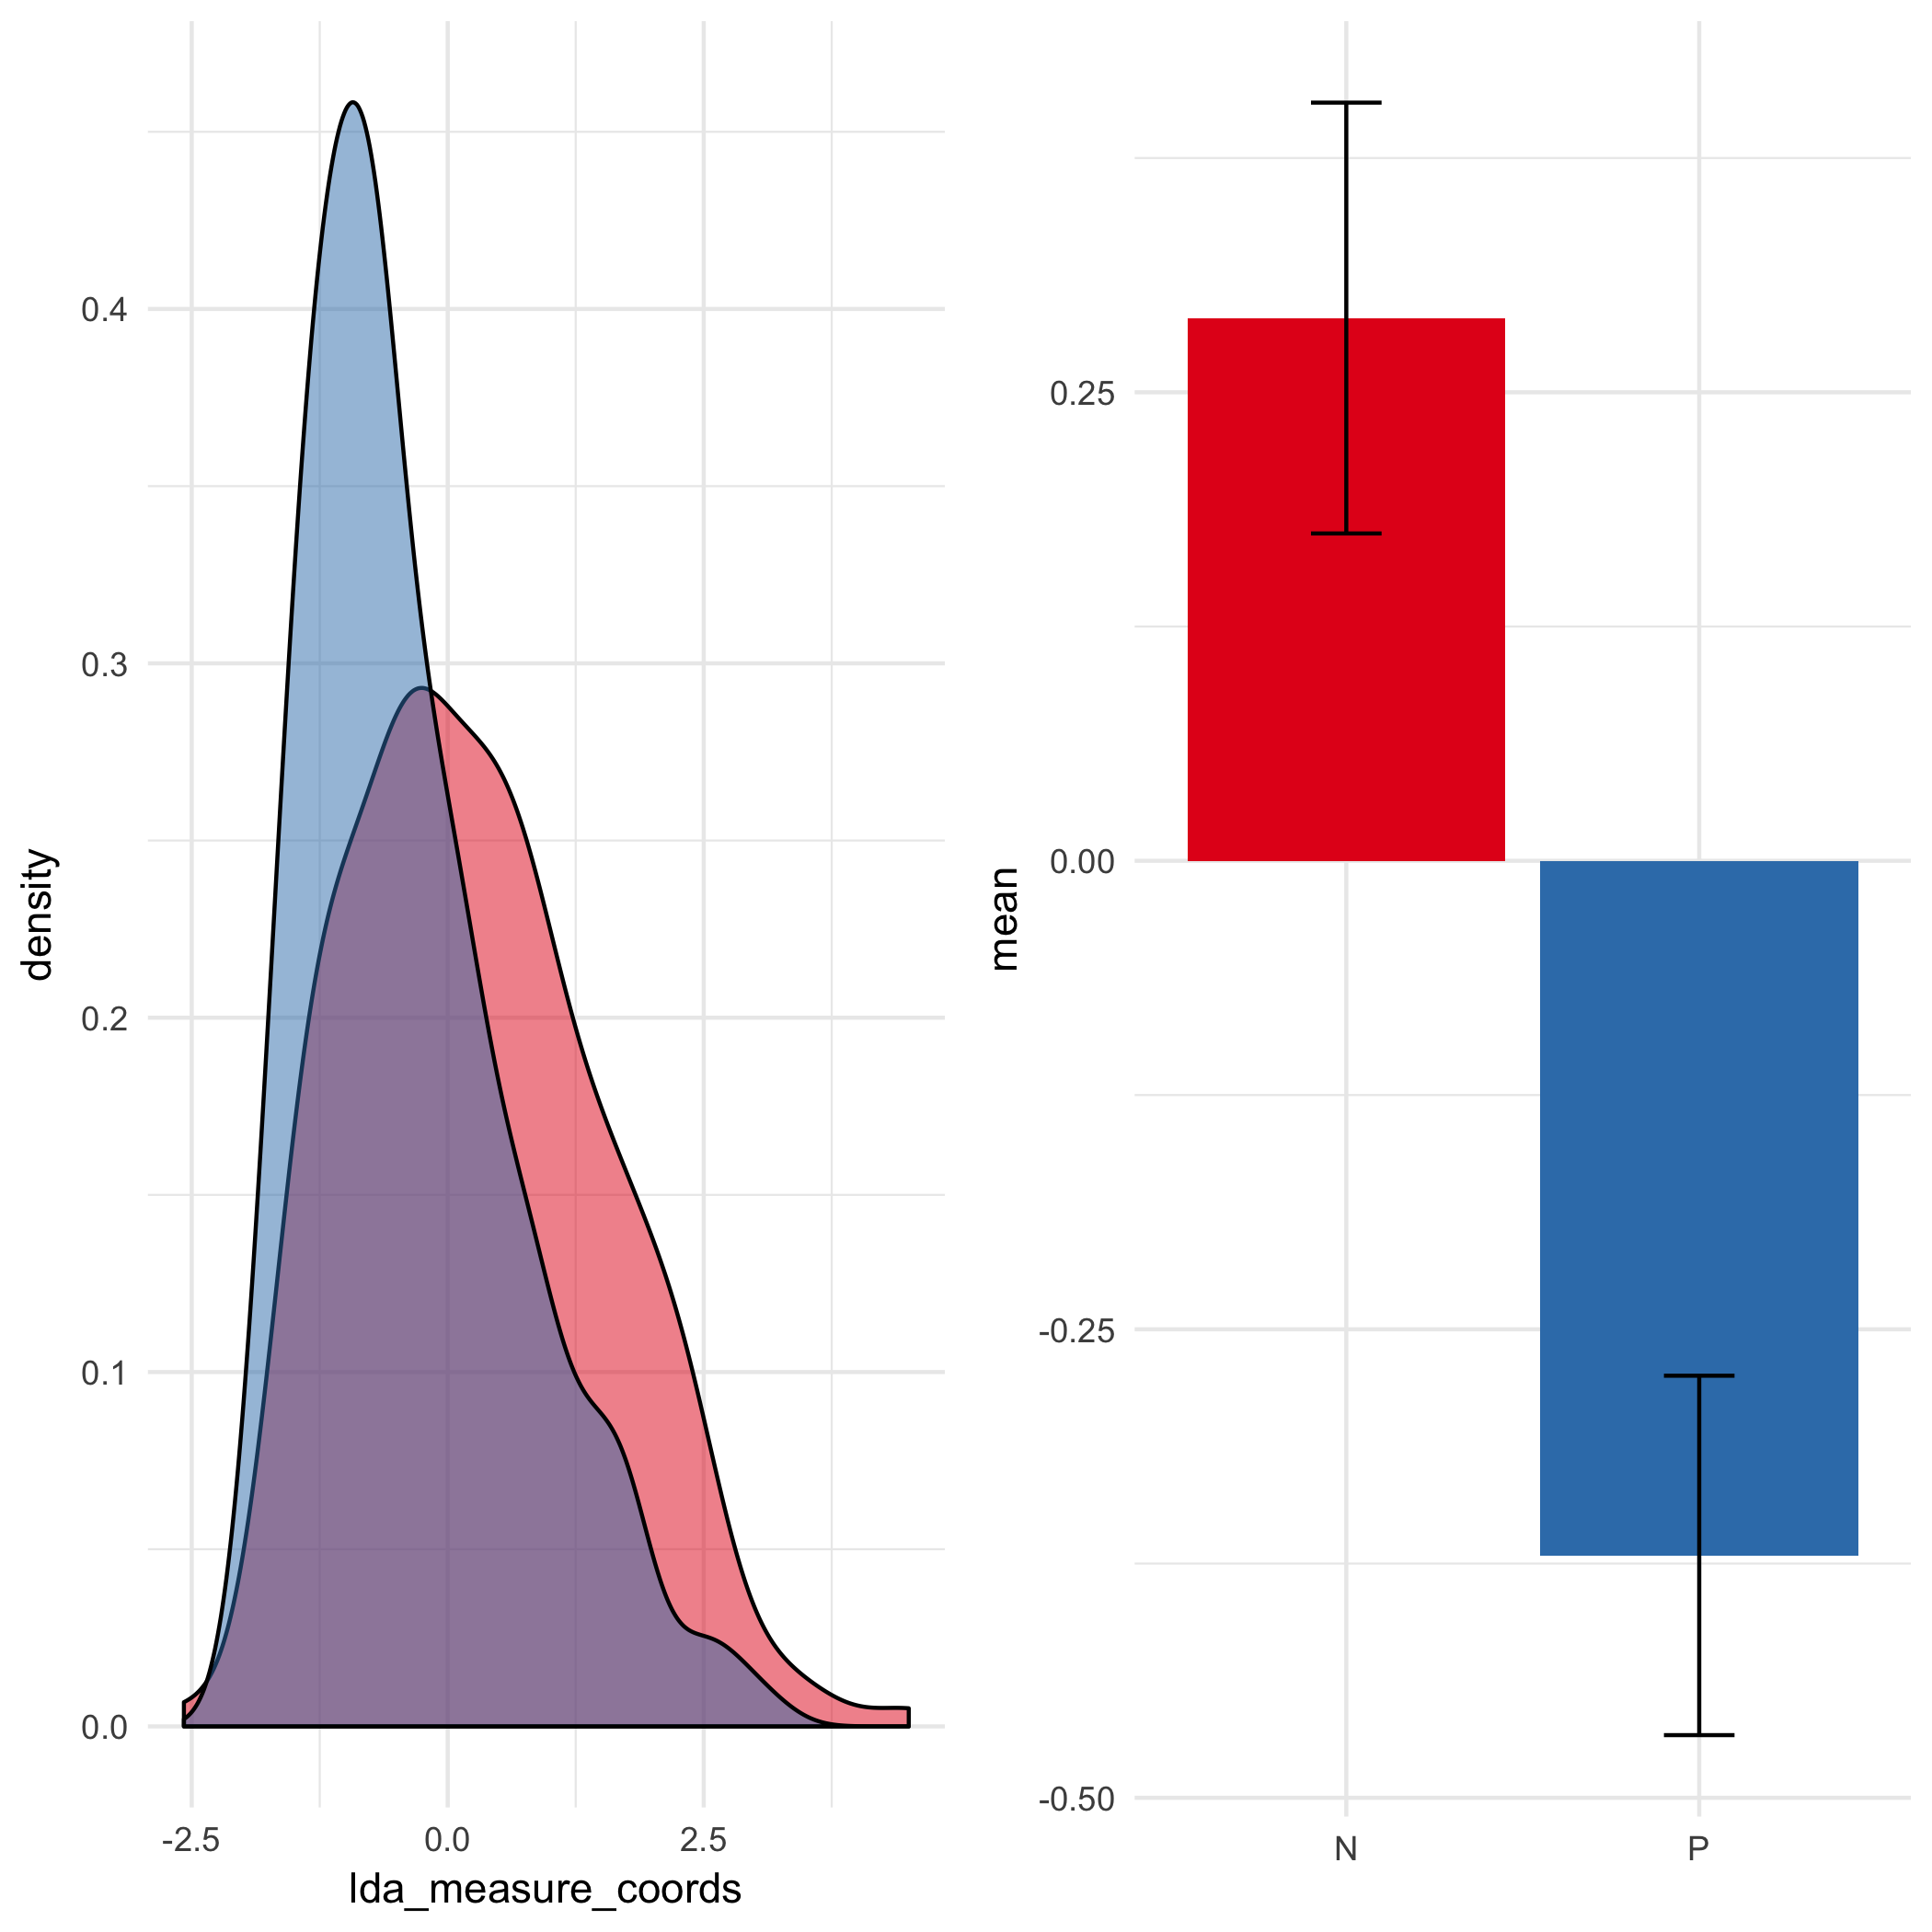
\includegraphics[width=\textwidth]{LDA-coords-negation.png}
\caption{LDA only with coordinates}
\end{subfigure}
\caption{Two LDA classifiers applied to \textit{true} trials. }
\label{fig:lda_negation}
\end{figure}

\end{itemize}


\paragraph{Measure comparison}
\begin{itemize}

\item What is the difference in performance between the different measures? (~Do the different measures differ on their ability to finding the effect when the effect is there?)  

\item Our results so far suggest that the LDA trained with validation data can distinguish negative and positive trials. The question that arises is whether this LDA classifier trained with controlled data can make a better distinction than other commonly used measures, such as the ones used by Dale and Duran. Indeed, it could be the case that the LDA classifier is only a better strategy than other measures when is trained and tested with an homogenous set of data (i.e. when training and testing sets correspond to the same type of decision processes). In other words, our classifier might not be able to extrapolate to different types of decision processes. 

\item \Cref{fig:different.measures.2} shows the results for values obtained for different measures for the contrast between positive and negative true statements. 

\begin{figure}
\centering
\begin{subfigure}[b]{0.4\textwidth}
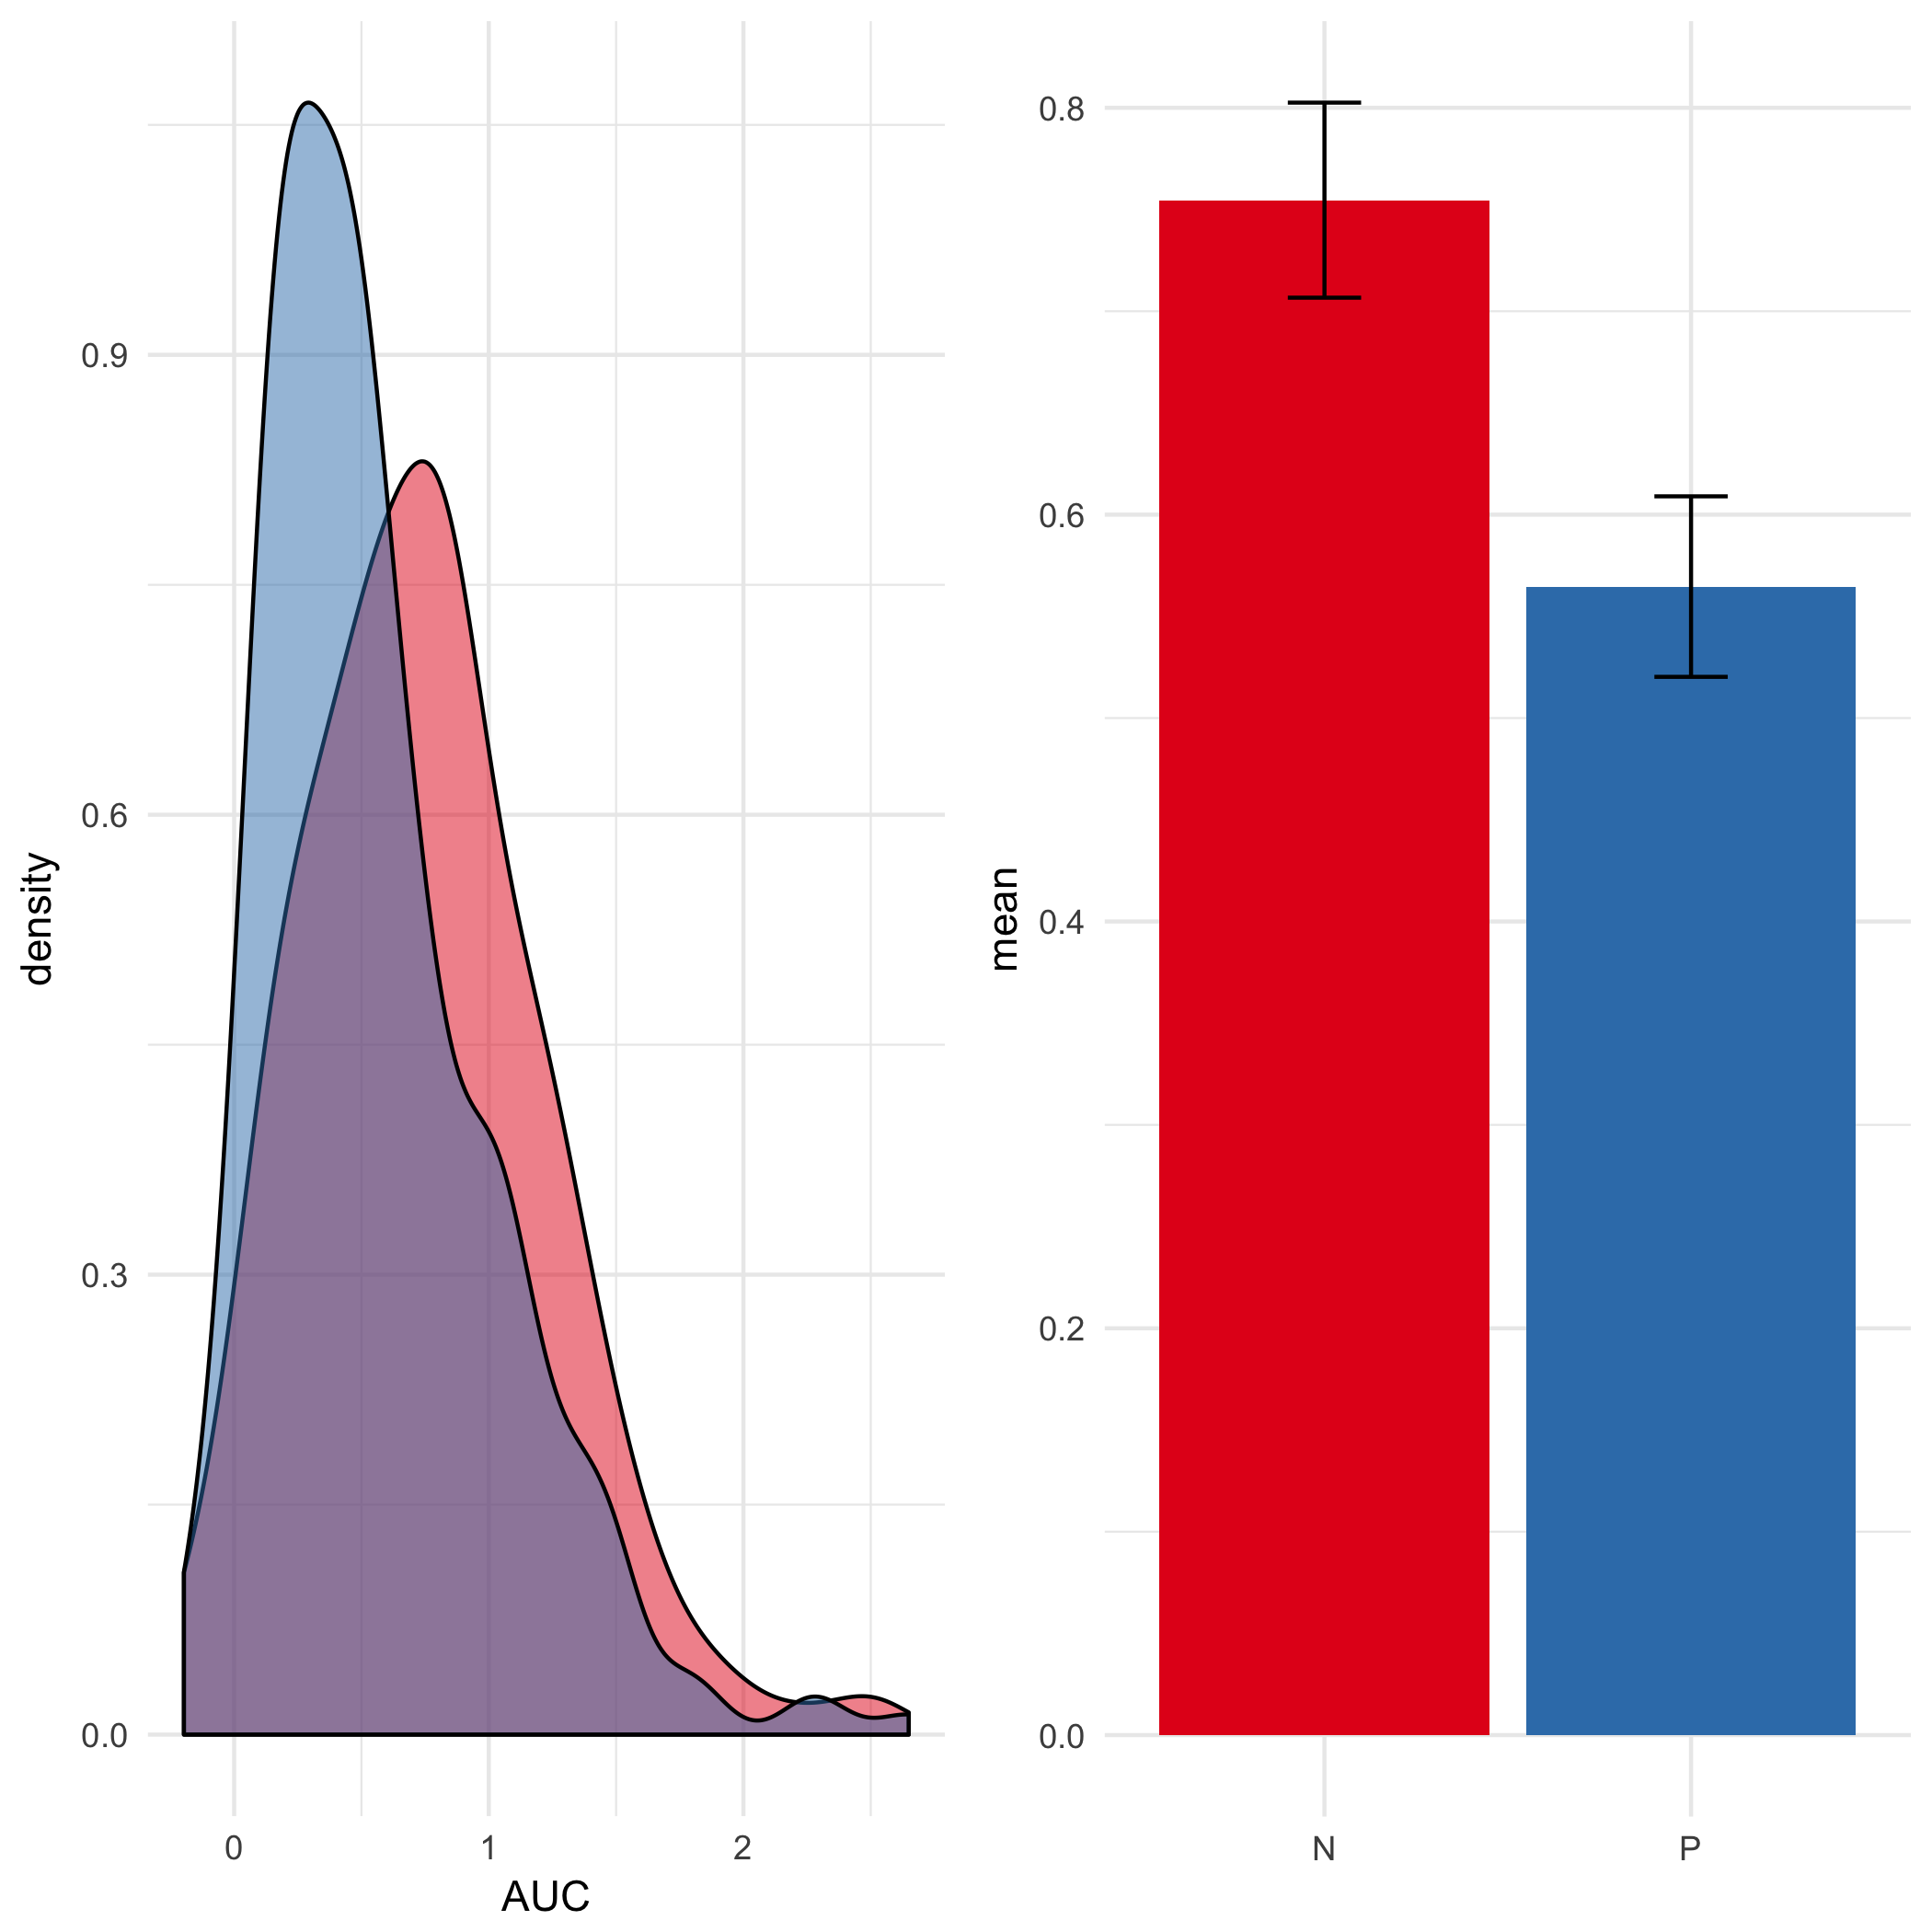
\includegraphics[width=\textwidth]{AUC-negation.png}
\caption{Area Under the Curve}
\end{subfigure}
%
\begin{subfigure}[b]{0.4\textwidth}
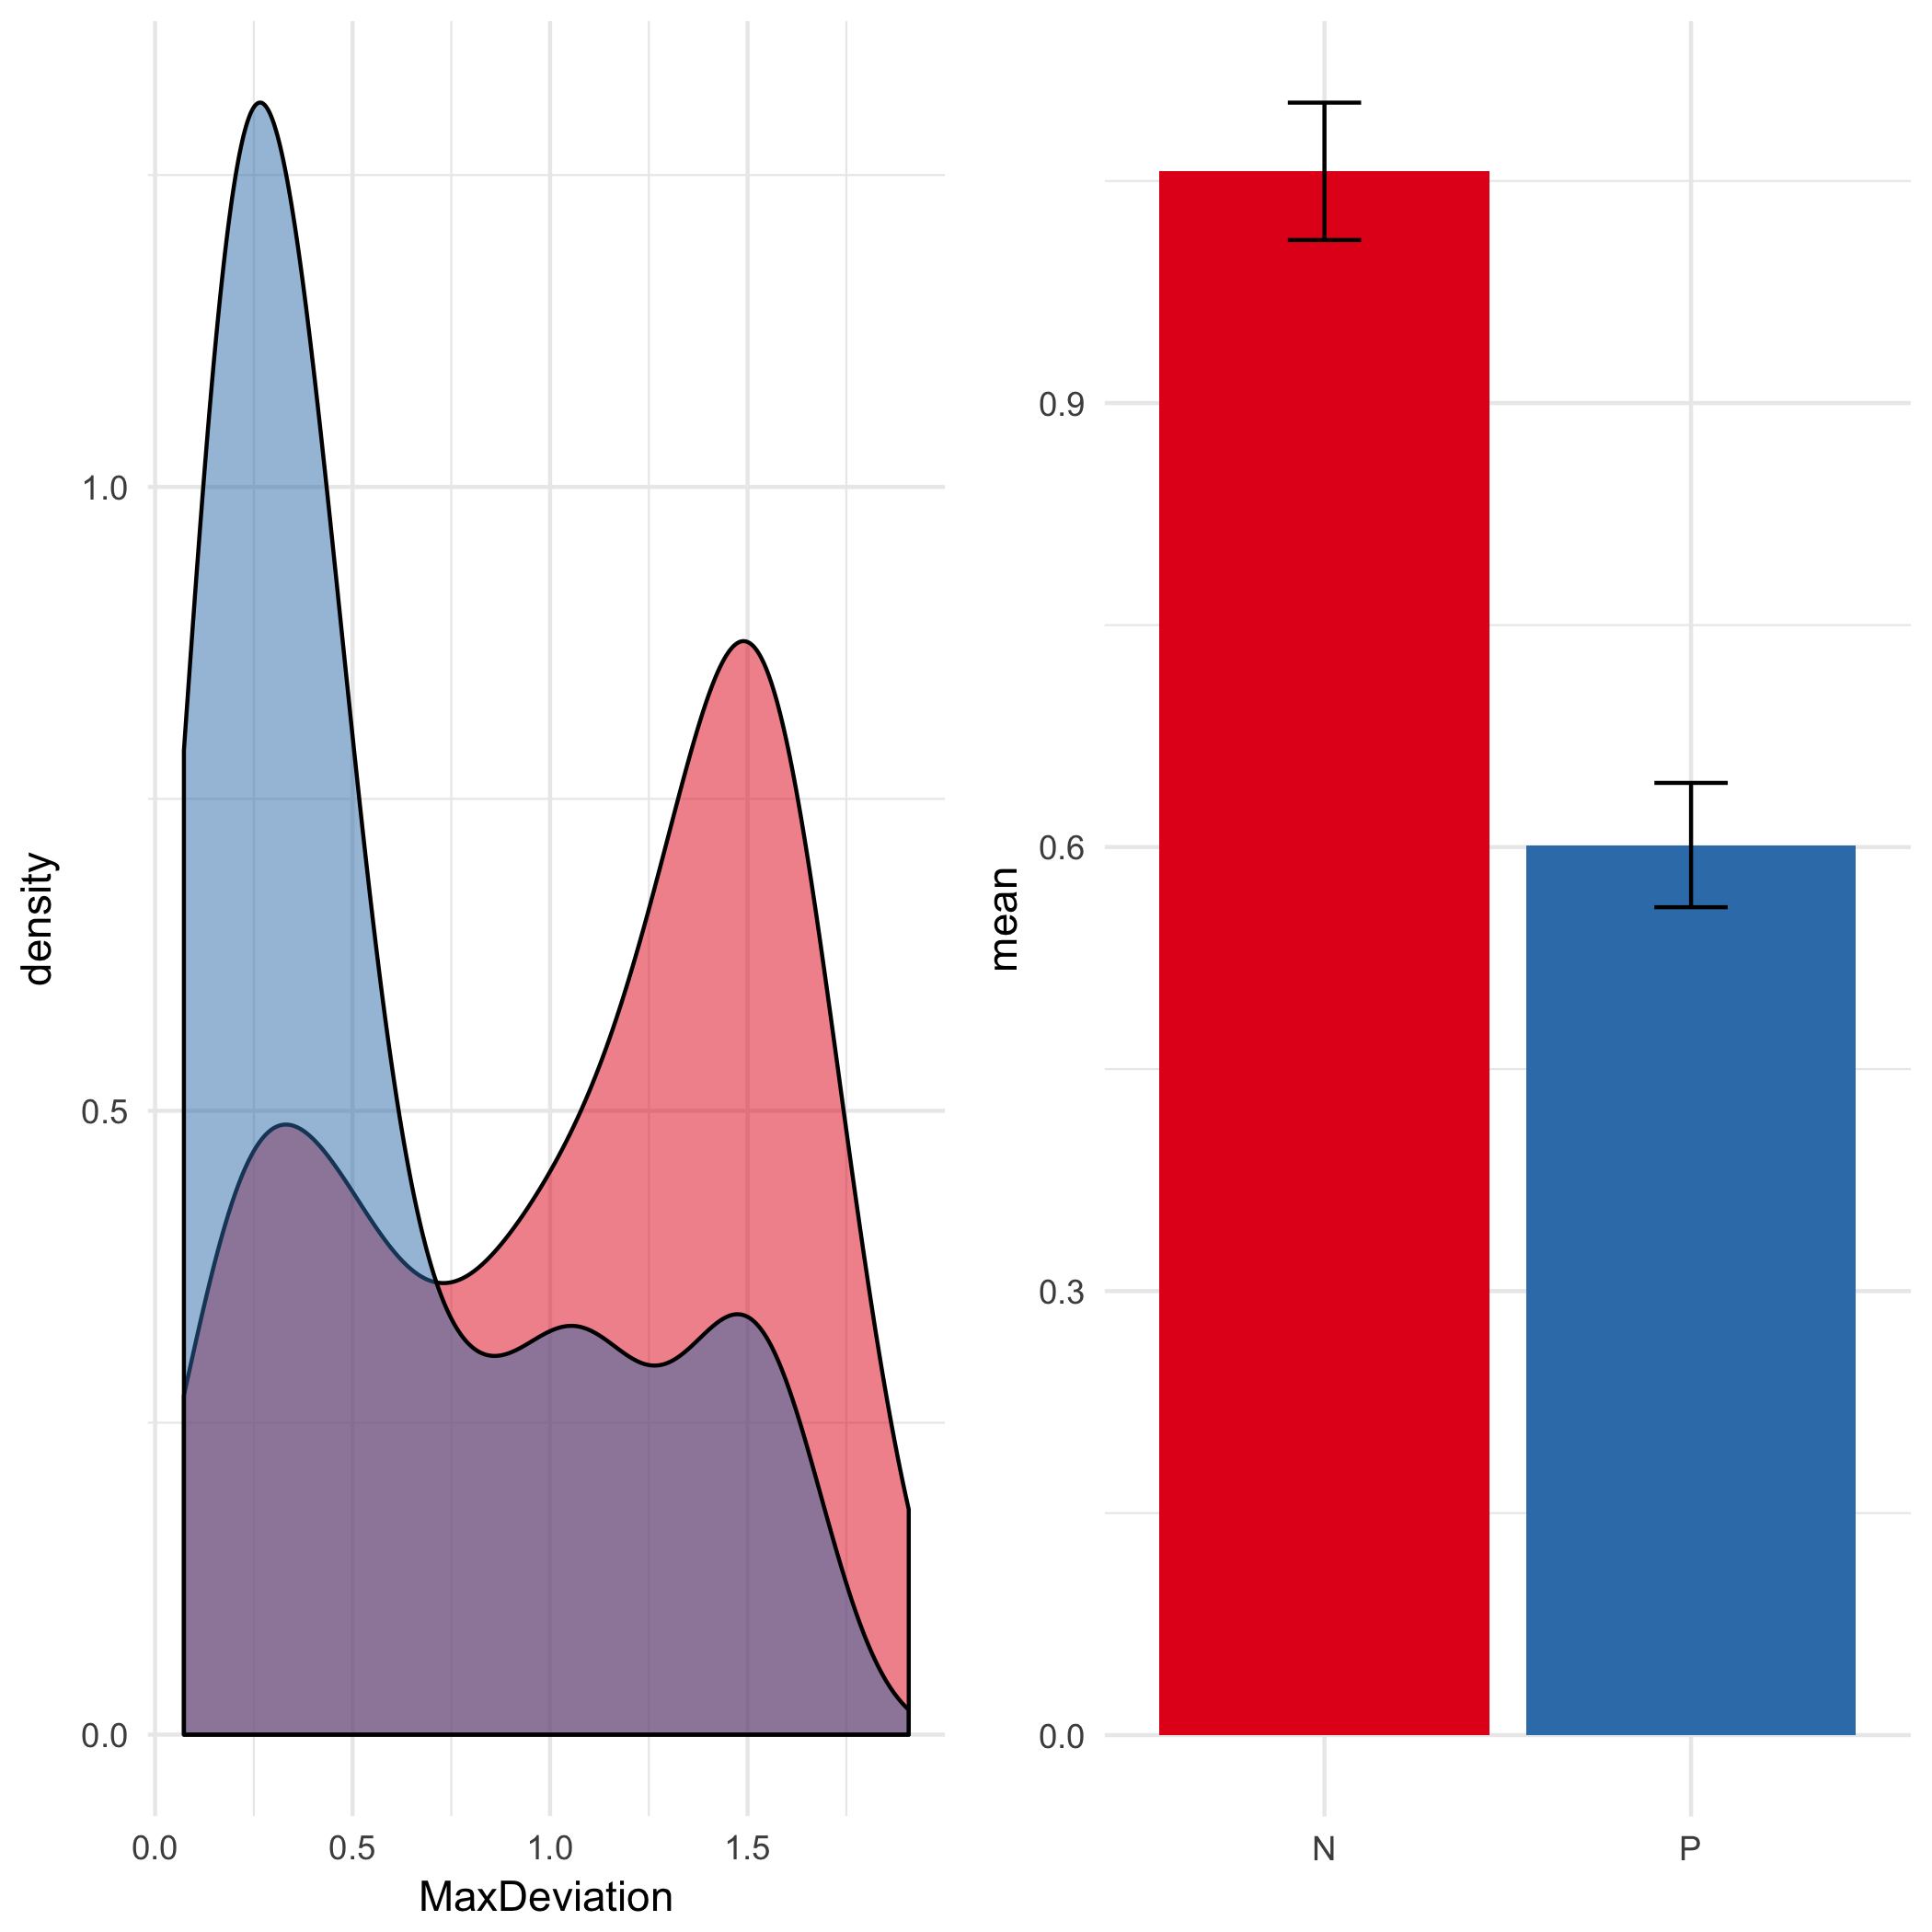
\includegraphics[width=\textwidth]{MaxDeviation-negation.png}
\caption{Maximal Deviation}
\end{subfigure}

%
\begin{subfigure}[b]{0.4\textwidth}
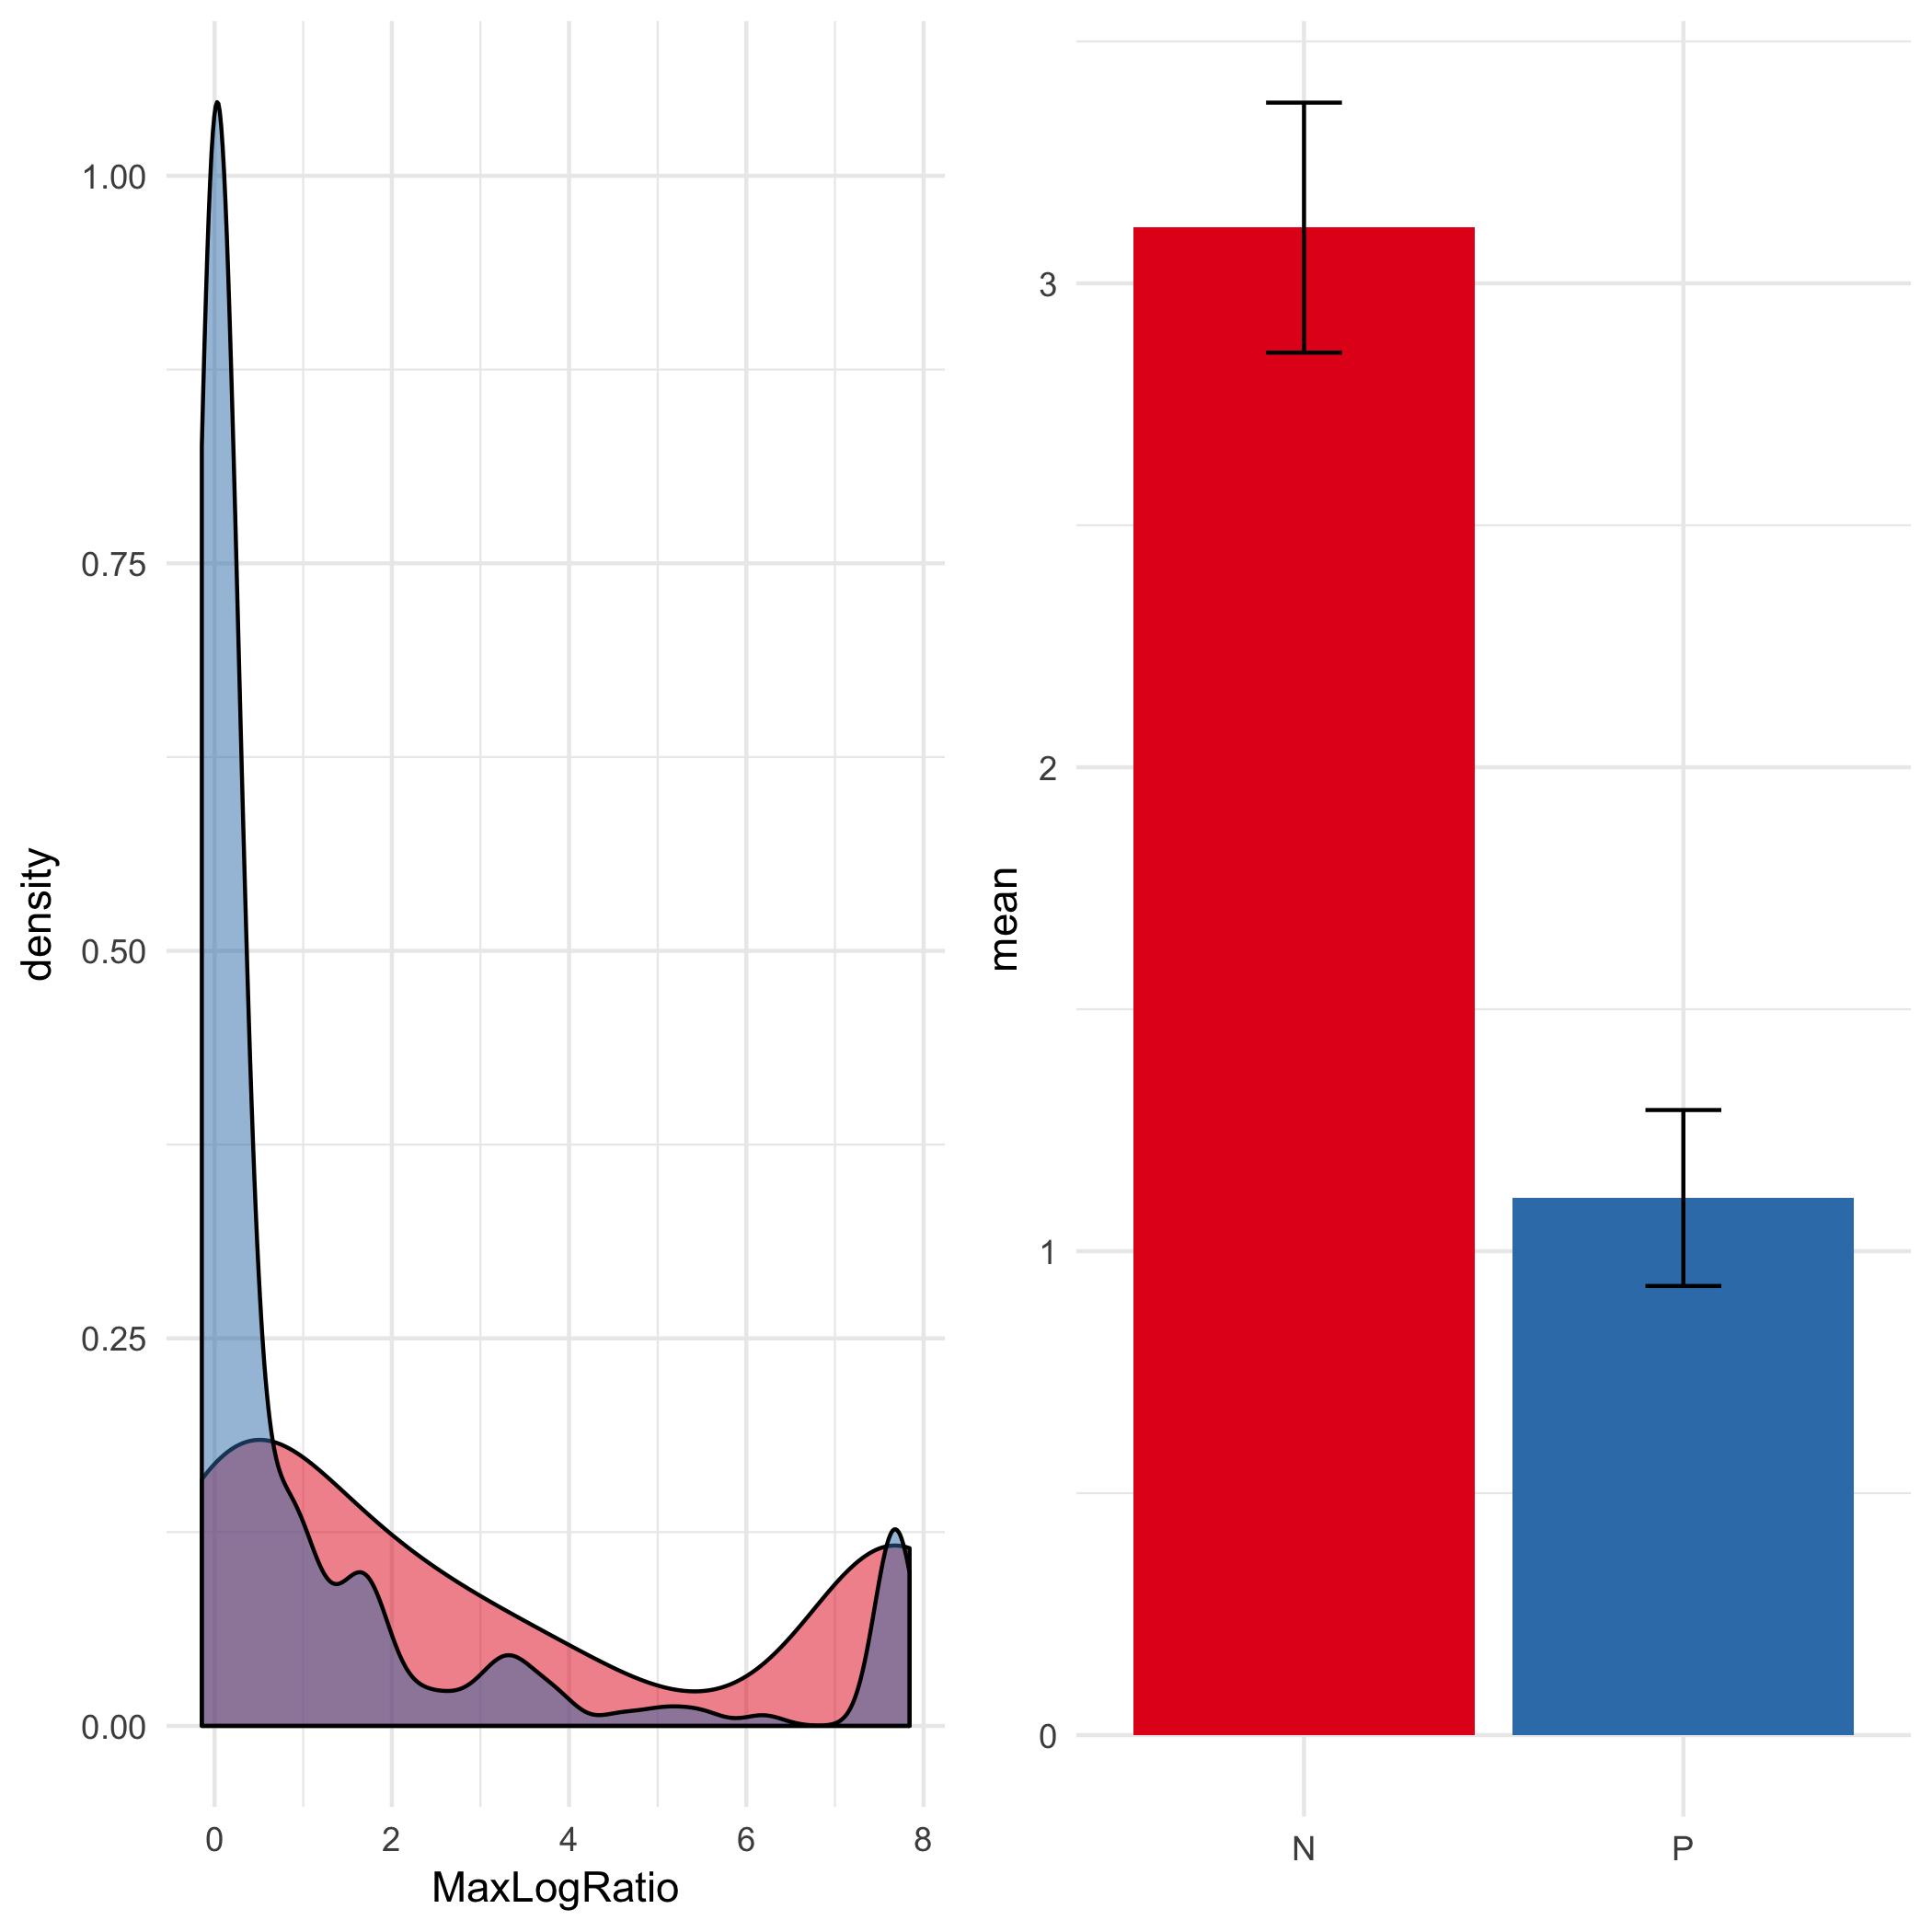
\includegraphics[width=\textwidth]{MaxLogRatio-negation.png}
\caption{Maximal LogRatio}
\end{subfigure}
%
\begin{subfigure}[b]{0.4\textwidth}
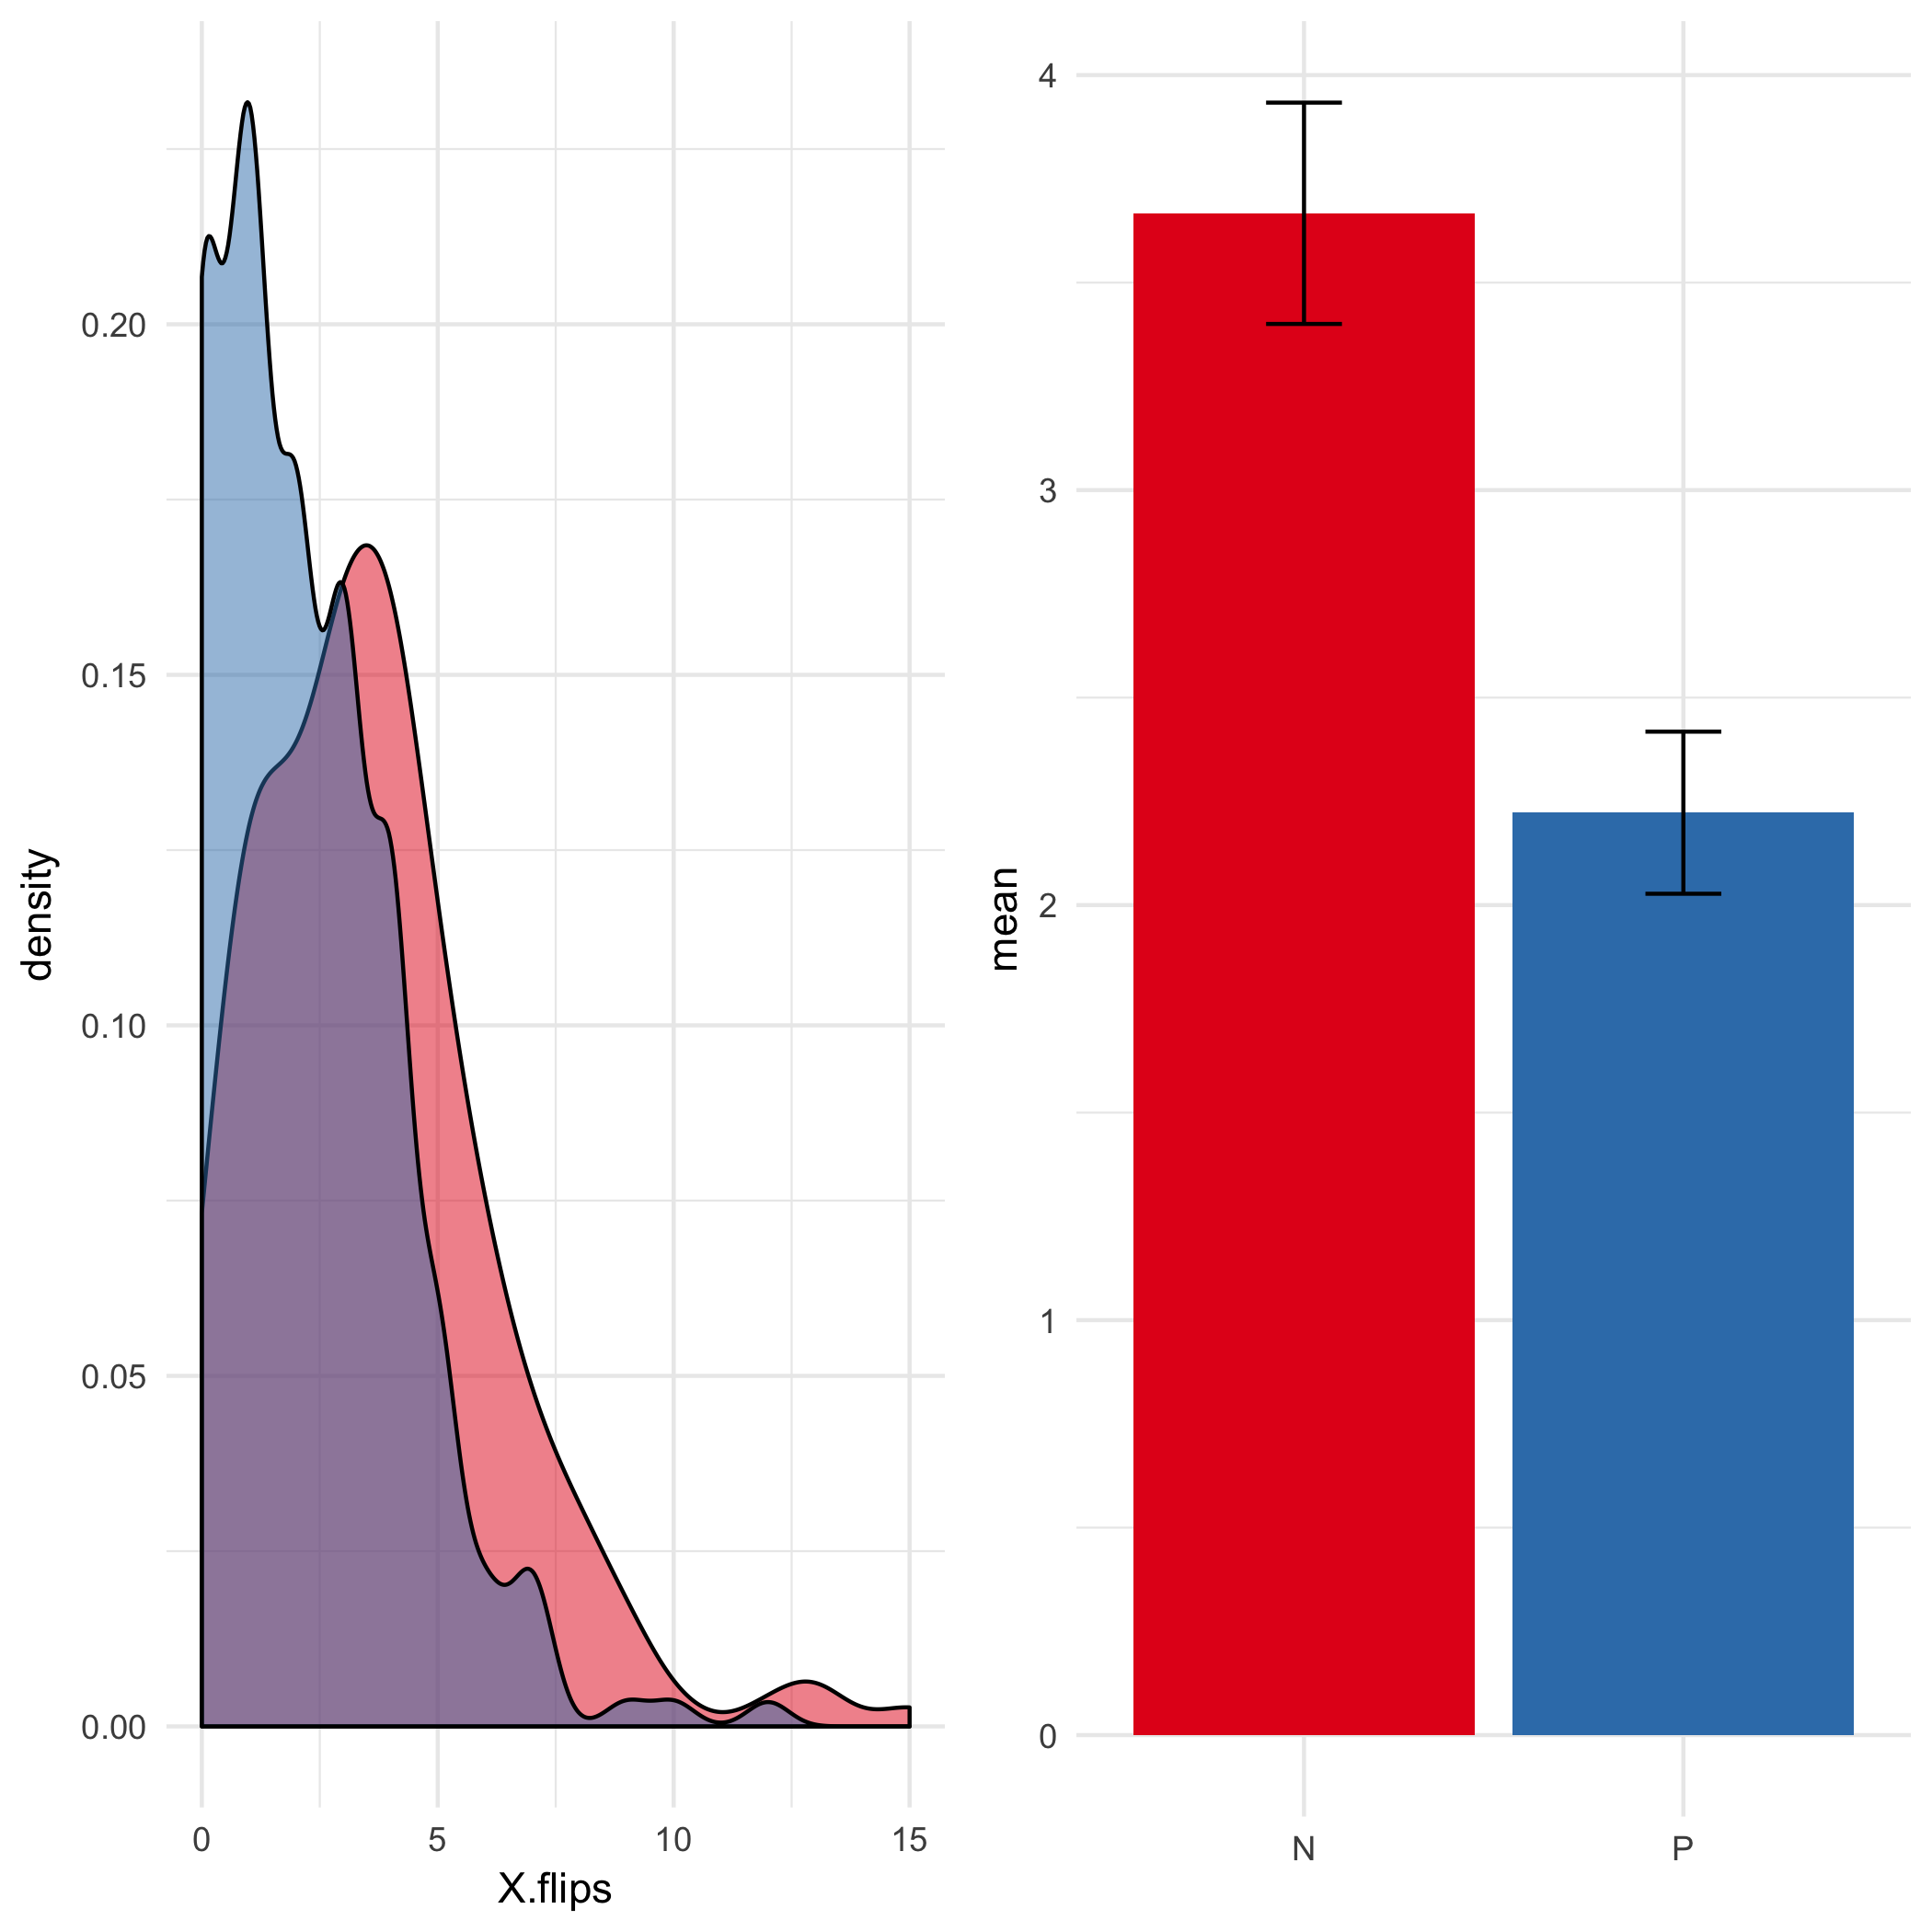
\includegraphics[width=\textwidth]{Xflips-negation.png}
\caption{X-coordinates Flips}
\end{subfigure}

\caption{Different measures applied to Dale \& Duran replication.}
\label{fig:different.measures.2}

\end{figure}

\item To estimate the power/robustness of these measures, we asked whether they could accurately detect the effect when we reduce the sample size. 
We calculate the area under the ROC curve for different sample sizes by bootstrapping from the original data set. \Cref{fig:power} shows a power curve: for each sample size the percentage of iterations where the AUC is above .5 (above random performance). \Cref{fig:means} illustrates the mean AUC values obtained for each sample size and each measure. 

\item The results in \Cref{fig:AUC.negation} suggests that: 
(a) none of the measures performs a classification as good as the one observed with validation data;  
(b) the ranking based on power does not correspond exactly to what we see in the AUC statistics (ie. how good they are at detecting the effect is not necessarily equivalent to having the highest AUC values):  
(i) the Original LDA is as powerful as the one of the Maximal Deviation and Maximal Log Ratio;
(ii) the AUC statistics suggest the existence of a ranking between these three measures such that Maximal Deviation gives rise to overall higher AUC values.  
(c) Finally, the performance of the Coords LDA, $x$-flips, the area under the curve seems to be weaker across the board. 

\item The LDA applied to the linguistic data is not as good as it was when applied to the validation data. This difference might be related with the fact that the two sets of data (training and testing sets) correspond to two different tasks, involving different decision processes. The decision processes involved in sentence verification tasks are much more complex than the ones targeted in our validation experiment. Consequently, the LDA model might not be as detailed/complex as it would be required in order to improve the classification of negation data (i.e. it has not been trained to pay attention to important aspects of decision dynamics). The fact that negation data are \textit{a priori} more complex additionally explains the overall drop in performance across different measures.  

\item From a practical point of view, our findings indicate that the contrast between processing/verifying negative and affirmative sentences can be detected in mouse trajectories by just using certain traditional measures such as the maximal deviation. In other words, it's is not required to use a LDA classifier. 


\begin{figure}
\centering
\begin{subfigure}[b]{0.4\textwidth}
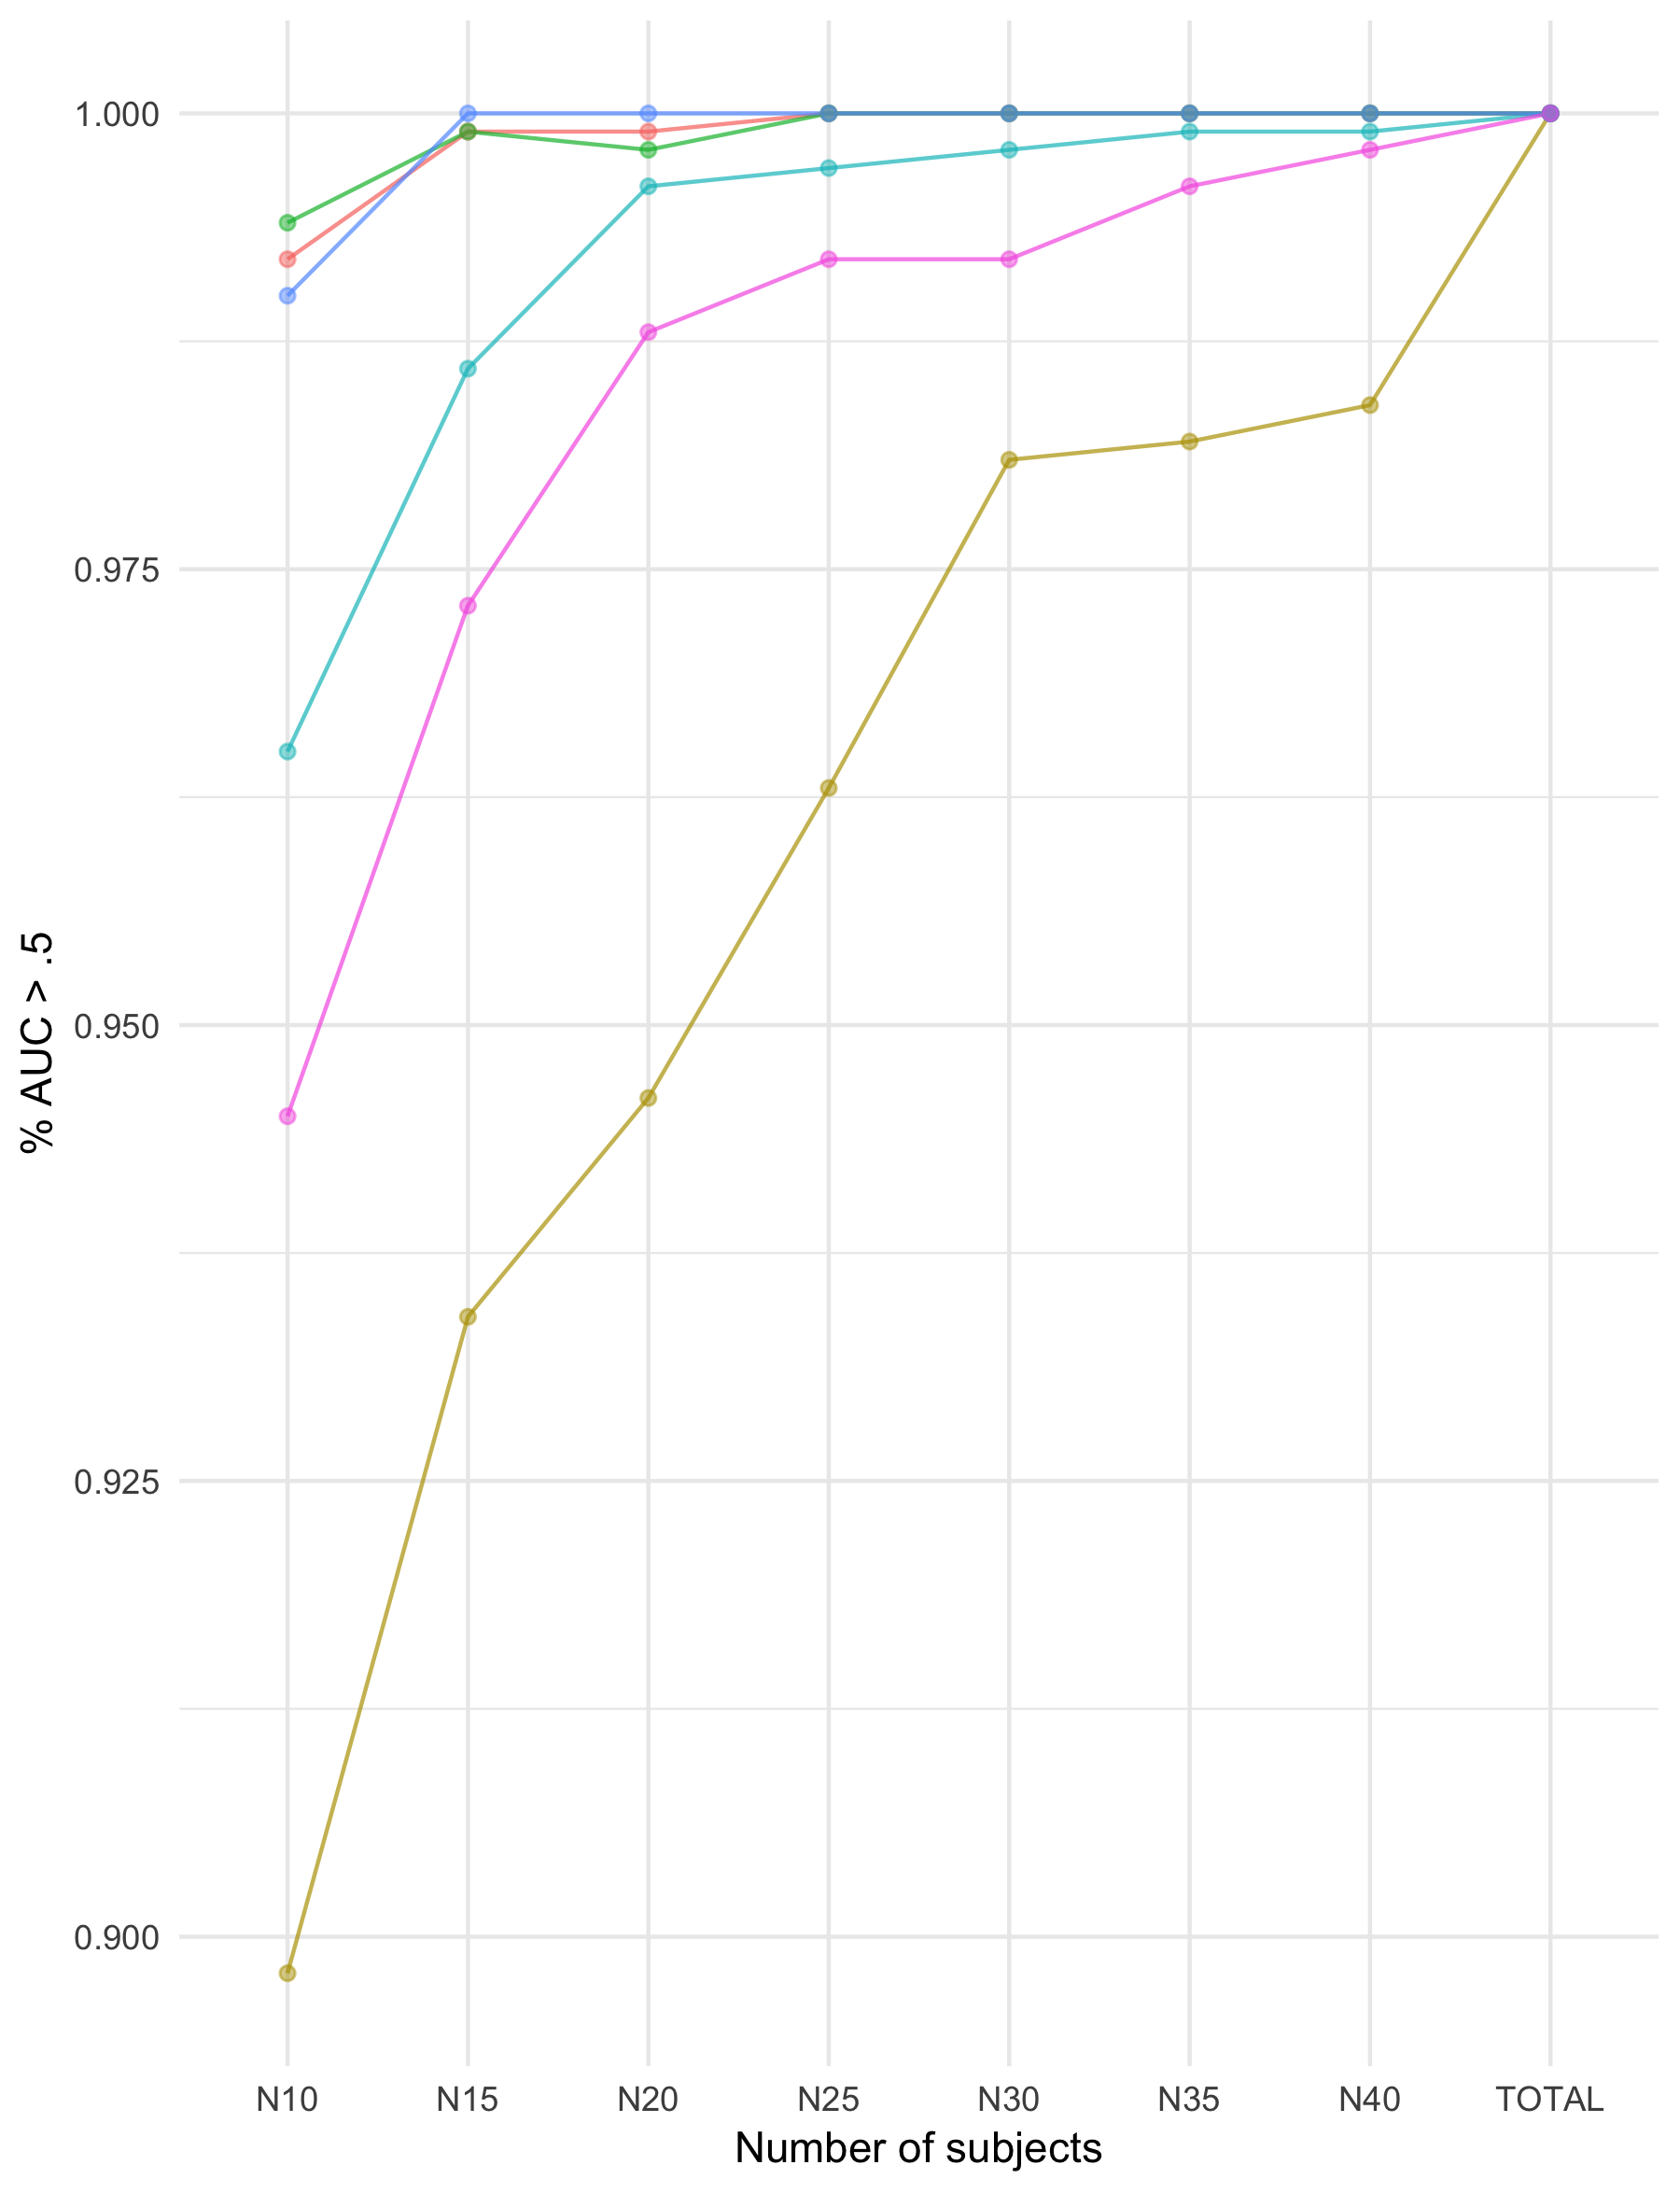
\includegraphics[width=\textwidth]{MeasurePower.png}
\caption{Power}\label{fig:power}
\end{subfigure}
\begin{subfigure}[b]{0.5\textwidth}
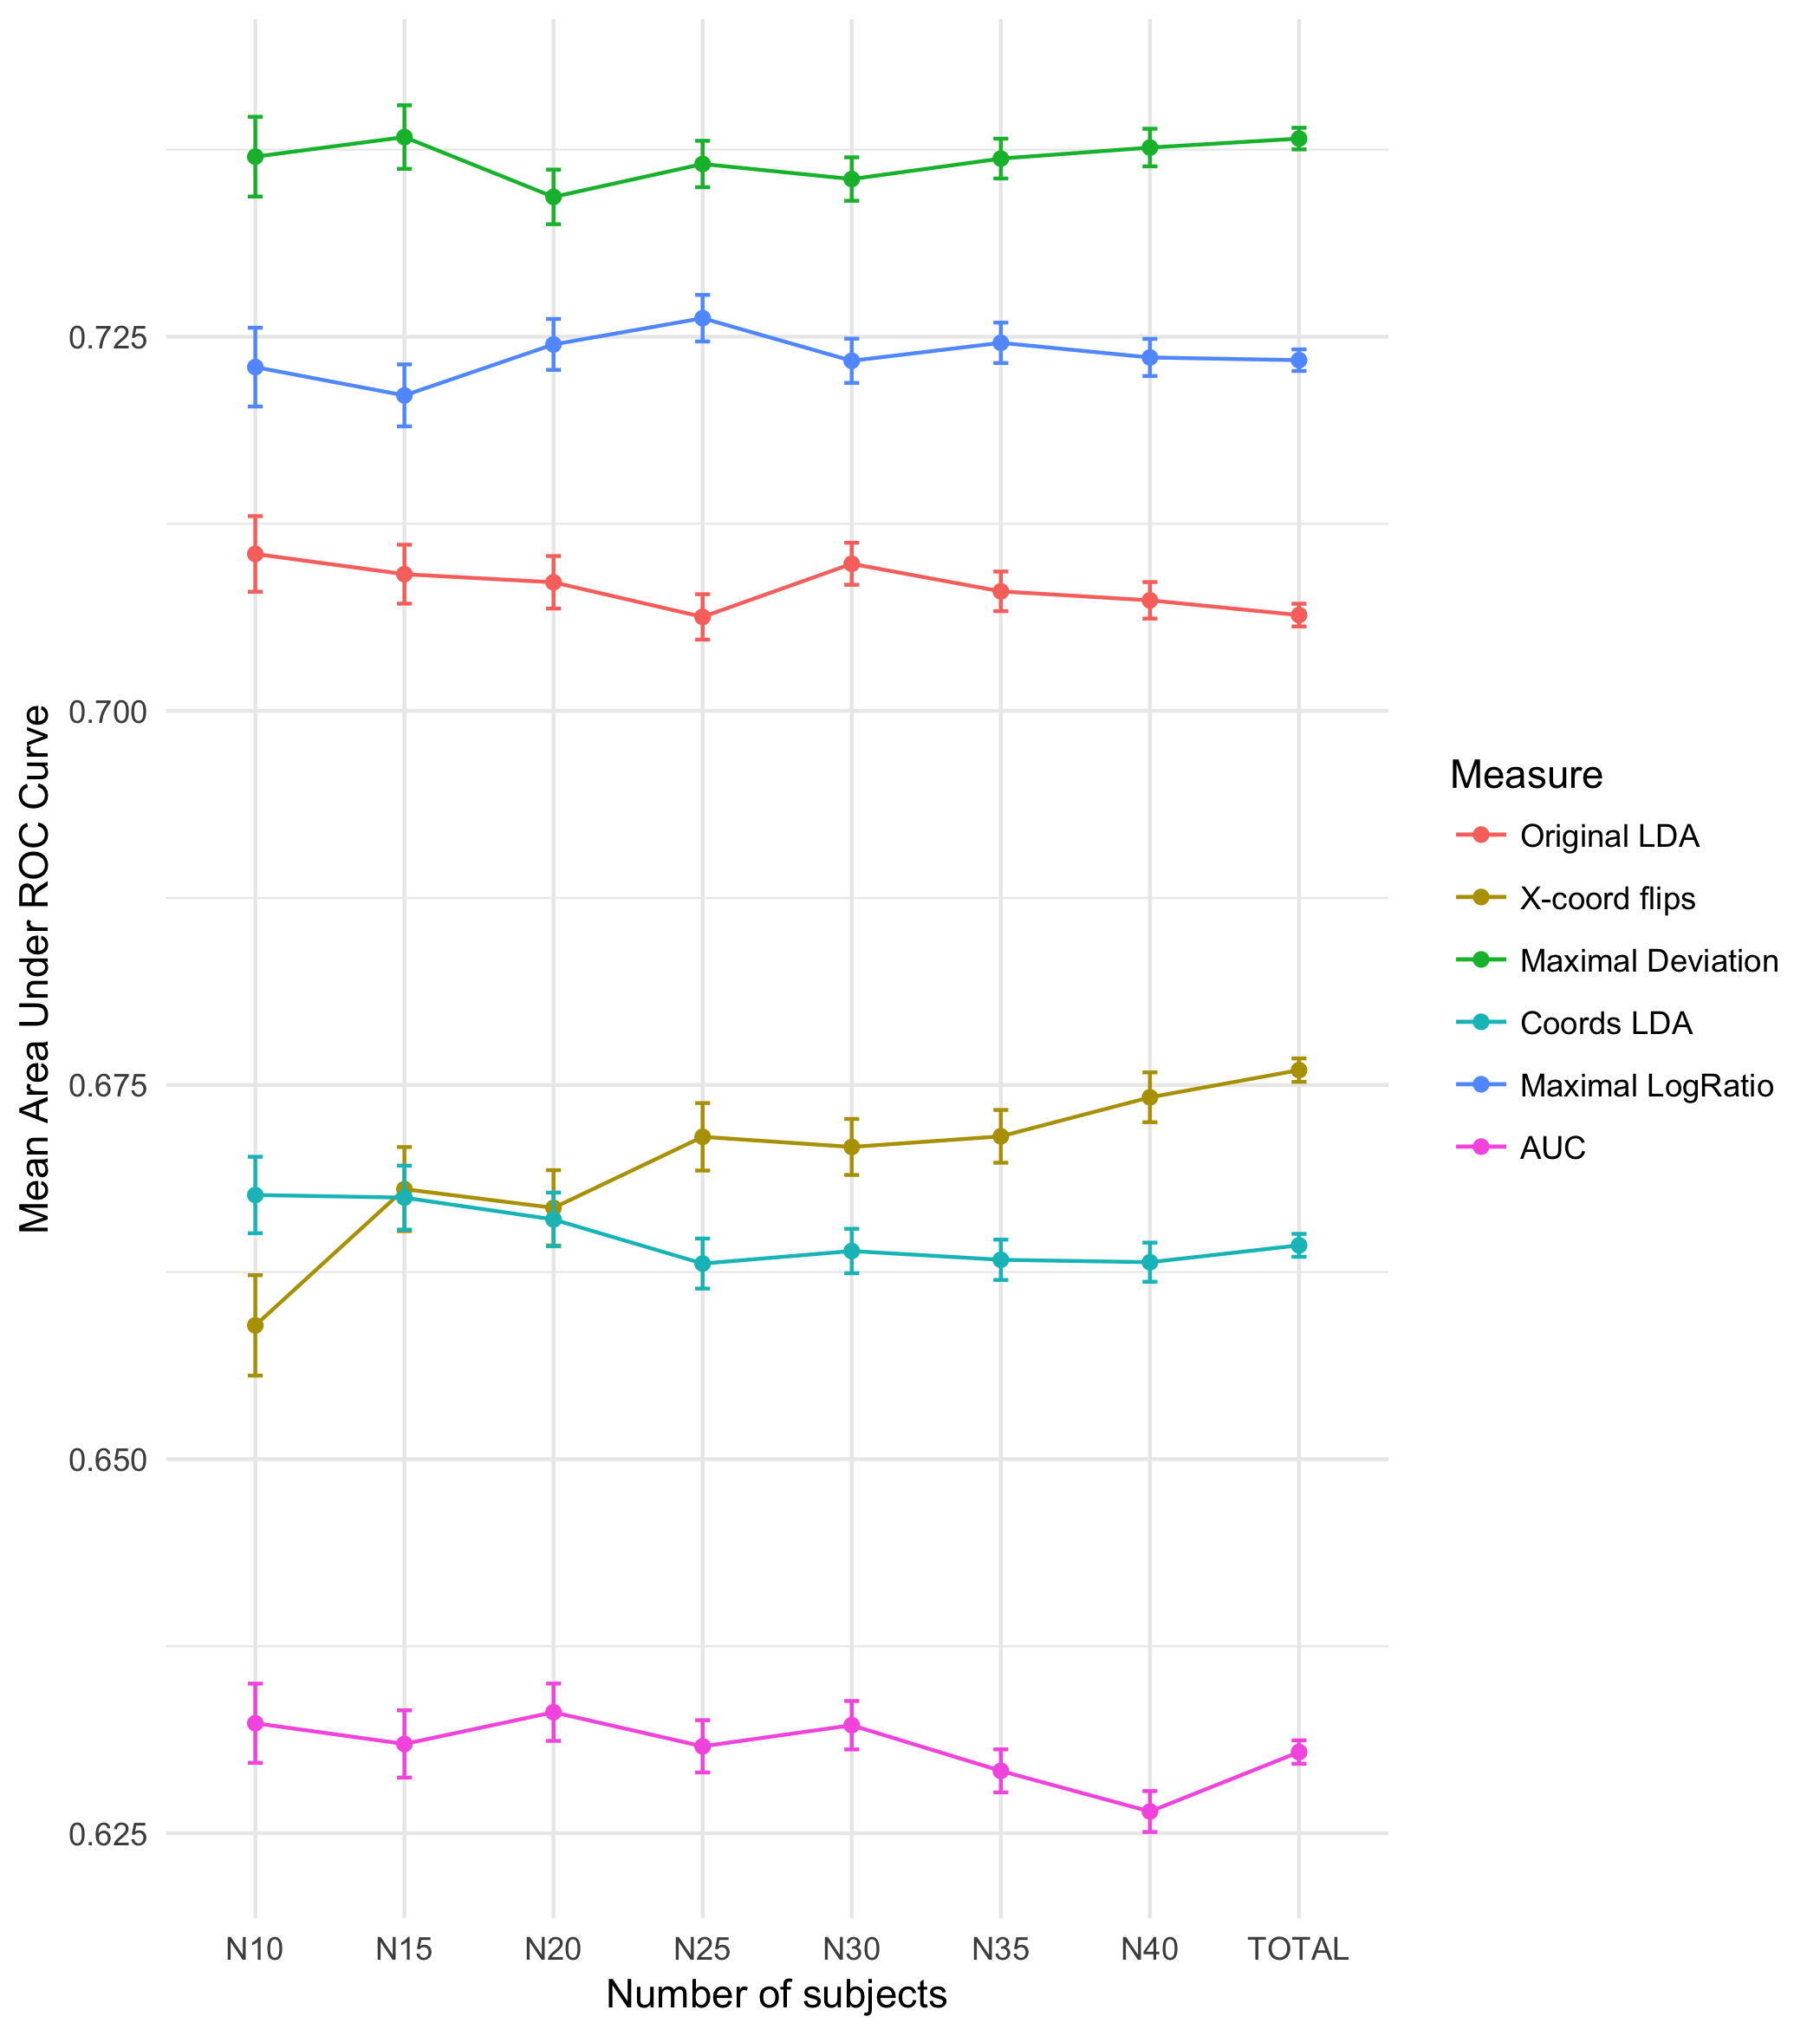
\includegraphics[width=\textwidth]{MeasureAUC_means.png}
\caption{Means}\label{fig:means}
\end{subfigure}
\caption{Measure performance for different sample sizes}\label{fig:AUC.negation} 
\end{figure}



\end{itemize}


\section{General Discussion}


\begin{itemize}
\item This study aimed to test the mapping from decision making to mouse movements. Our results make the following contributions:

\item By manipulating whether the stimulus triggered or not a change of decision, we have shown that mouse trajectories capture differences in decision dynamics. 
That is to say, when participants are forced to switch their decision, this change has a direct repercussion in their hand movements.  

\item We have demonstrated that mouse trajectories underlying each type of decision process can be distinguished by a LDA classifier. In order to make such distinction, this classifier can rely only on absolute temporal and spatial information about the position of the mouse at each time step, without taking into account relative information about how the mouse got there (speed and acceleration).
Our LDA classifier not only has a better performance than more traditional mouse-tracking measures but also has the advantage of being able to make a distinction without making any specific assumption about how trajectories should look like.     

\item We replicated Dale and Duran findings regarding negation processing. The result of applying our LDA classifier, trained on validation data, to data obtained from a sentence verification task suggest that processing negative sentences involves a change of decision, absent during the verification of positive sentences. 

\item Although the LDA manages to dissociate between these two sentence verifications, its performance is overall lower than in the validation case, and not significantly different from the one of other traditional measures. 

\item The difference LDA performance across experiments reveals that the two data sets 
are capturing slightly different decision processes. Ideally, we should be able to make our validation experiment slightly more complex in order to capture subtleties.  


\end{itemize}


\section{Supplementary materials}

\begin{itemize}
\item Time information for validation experiment


\begin{figure}
\centering
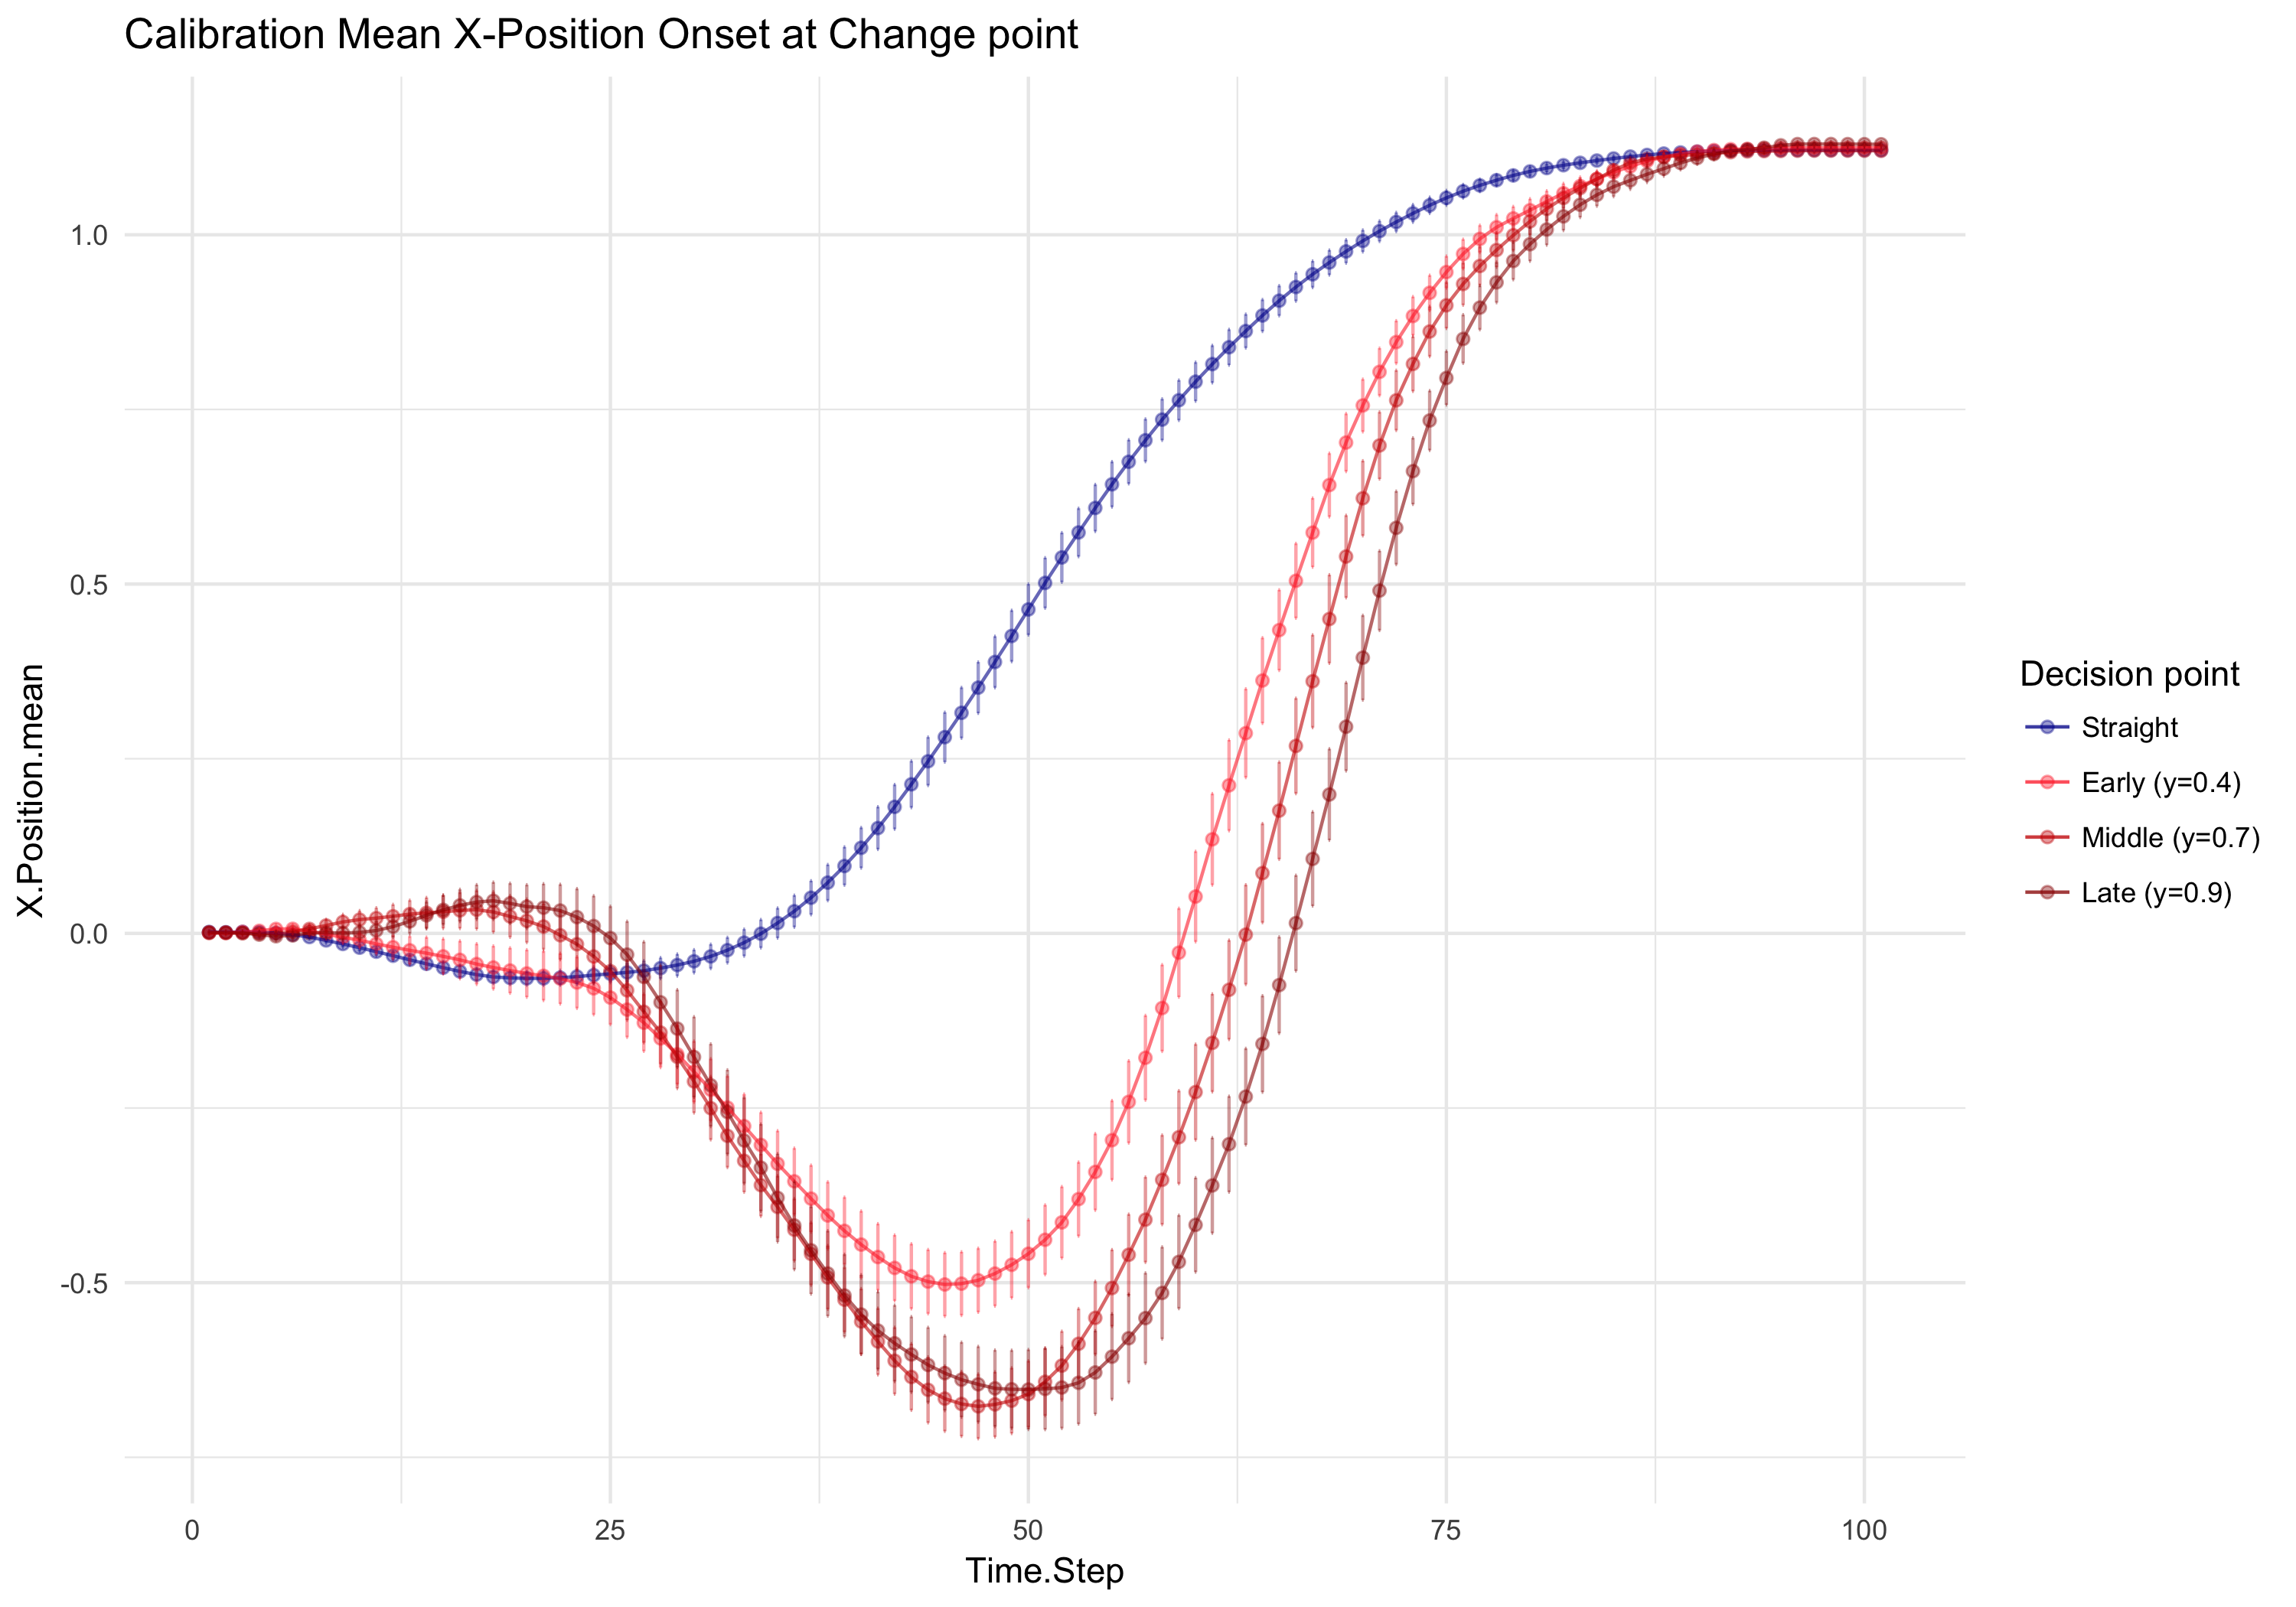
\includegraphics[width=0.5\textwidth]{calibration_mean_XPosition_time.png}
\caption{}
\end{figure}

\item Other LDA with different predictors: Another two classifiers were trained with a different set of predictors. A first one had as predictors $x,y$ coordinates and partial derivatives: vertical velocity and acceleration ($y$-based) and horizontal velocity and acceleration ($x-$based). 
Spatial and temporal features for each axis might predict the type of decision to a different extent \addMM{(both axes might be relevant but to different extent)}. 
For instance, the movement on the horizontal axis might have stronger relevance for the classification than the movement on the vertical axis.  
A second classifier had as predictor the ratio between the euclidean distance to the alternative response and the distance to the target response. \addMM{The ratio contains spatial information, but it is sensitive to how close the point was to the target response and to the alternative.} \addMM{Add results}


\end{itemize}





\end{document}